\documentclass[11pt]{article}
\usepackage[utf8]{inputenc}
\usepackage[
papersize={5.5in, 8.5in},
left=0.35in,
right=0.35in,
top=0.35in,
bottom=0.5in]{geometry}
\usepackage{moresize}
\usepackage{graphicx}
\usepackage{amsthm}
\usepackage{rotating}
\usepackage{amsfonts,amssymb,amsmath}
\usepackage[usenames]{color}
\usepackage[T1]{fontenc}

\usepackage{longtable}
\usepackage{array}
\usepackage{float}
\usepackage{booktabs}
\usepackage[dvipsnames,usenames,table,xcdraw]{xcolor}

\renewcommand{\Re}{\mathop{\mathrm{Re}}\nolimits}
\renewcommand{\Im}{\mathop{\mathrm{Im}}\nolimits}

\newcommand{\gr}{\cellcolor[HTML]{E0E0E0}}
\newcommand{\tbd}{\vspace{7cm}}
\newcommand{\m}{\bf}
\newcommand\T{\rule{0pt}{2.5ex}}       % top strut
\newcommand\B{\rule[-0.7ex]{0pt}{0pt}} % bottom strut
\newcommand{\comment}[1]{}
\newcolumntype{P}[1]{>{\centering\arraybackslash}p{#1}}
\newcommand\myfontsize{\fontsize{15pt}{18pt}\selectfont}

\DeclareMathOperator{\Aut}{Aut}
\graphicspath{ {images/} }
\newtheorem*{theorem}{Theorem}
\newtheorem{conj}{Conjecture}
\frenchspacing
\setcounter{secnumdepth}{3}
\parskip=1mm
 
\title{\bf %\Green
%Simple bounds for the chromatic number of the plane with the set of forbidden distances
More certainty in coloring the plane with a forbidden distance interval
}
\author{\bf %\normalsize 
\textcolor[rgb]{0,0.8,0.8}{Jaan Parts} \\
} 
%\date{\today}
\date{\normalsize \textcolor[rgb]{0,0.8,0.8}{Kazan, Russia, jaan\_parts@.mail.ru}}

\begin{document}

\maketitle

\pagestyle{empty}
\thispagestyle{empty}

\begin{abstract}
In the mysterious and colorful world of chromatic numbers, where there are a lot of unknown, there is an amazing thing. It turns out that for some intervals of forbidden distances on the plane, one can specify the exact value of the chromatic number $\chi$. Two sets of such intervals have been found, for $\chi=7$ and 9. We call them islands of certainty. Here we increase the size of these islands, and add three new ones with $\chi=8$, 12, 13. We also %formulate conjectures which predict 
conjecture islands for $\chi=14$, 15, 16. Are there islands of certainty for $\chi$=10 or 11? This is still a mystery. Roll up for the Mystery Tour.
\end{abstract}

\section{Introduction}
\label{introduction}

Having knowledge regarding causal relationships rather than statistical associations enables us to predict the effects of actions that perturb an observed system \citep{TheBookOfWhy}. Determining causal structures is a fundamental problem in numerous scientific fields \citep{Rubin}. However, different data-generating processes can produce the same observational distribution. Observing the system after interventions is a reliable means to identify the causal structure, but in numerous real-life scenarios, interventions can be too expensive, unethical \citep{epidem_application}, or impossible to observe. Hence, estimating the causal structure from observational data has become an important topic.

In the last few decades, much effort has been put into developing a  mathematical background for a ``language'' of causal inference, centered around the structural causal model (SCM) \citep{Pearl_book}. Given a set of random variables $\textbf{X} = (X_1, \dots, X_d)^\top\in\mathbb{R}^d$, a SCM with an underlying acyclic graph $\mathcal{G}$ represents a data-generating process where the variables arise from structural equations 
\begin{equation*}
    X_i=f_i(\textbf{X}_{pa_i}, \varepsilon_i),\,\,\,\,\,\,\,\,\, \,\,\,\,\,\,\,i=1,\dots, d, 
\end{equation*}
where $f_i$ are the causal (link) functions, $pa_i$ represent the parents (direct causes) of $X_i$ in $\mathcal{G}$, and $\varepsilon_i$ are jointly independent noise variables. The fundamental goal of causal discovery is to estimate the causal structure (causal graph $\mathcal{G}$).  It is straightforward to compute the distribution of $\textbf{X}$ if the graph $\mathcal{G}$ and the conditional densities are given. Here, we deal with the opposite problem, where the distribution of $\textbf{X}$ (or a random sample) is given and we want to infer $\mathcal{G}$. This task is typically impossible without strong assumptions on the SCM \citep{Elements_of_Causal_Inference}. 

The existing literature in the field presents numerous methods and corresponding results for causal discovery under various assumptions on the Structural Causal Model (SCM) \citep{ZhangReview}. When observing multiple environments following different interventions, the assumptions can be significantly less restrictive \citep{Peters_invariance, Multiple_contexts_Mooij}. However, if the goal is to uncover causal relationships based solely on an observed random sample, the assumptions become more strict; typically assuming additive noise \citep{Lingam, Peters2014, reviewANMMooij}. This assumption of additivity $X_i = f_i(\textbf{X}_{pa_i}) + \varepsilon_i$ suggests that $\textbf{X}_{pa_i}$ influences only the mean of $X_i$, while the tail, variance, and higher moments remain fixed. This is a strong assumption, as the tail or other characteristics of the random variable can provide different information about the causal structure.

In this paper, we develop a framework where $\textbf{X}_{pa_i}$ can arbitrarily affect the mean, variance, tail, or other characteristics of $X_i$. However, a caution has to be taken because if the model is too general, the causal structure will become unidentifiable, meaning that multiple causal structures could produce the same distribution of $\textbf{X}$.
\begin{example}\label{Gaussian case}
    A useful model that allows an arbitrary effect on the variance as well as on the mean is $X_i\mid \textbf{X}_{pa_i}\sim N\big(\mu(\textbf{X}_{pa_i}), \sigma^2(\textbf{X}_{pa_i})\big)$ for some functions $\mu, \sigma$, in which case the structural equation has the form 
\begin{equation*}\label{prva_gaussian_equation}
X_i =  \mu(\textbf{X}_{pa_i})+ \sigma(\textbf{X}_{pa_i})\, \varepsilon_i, \,\,\,\,\,\,\,\,\,\,\varepsilon_i\text{ is Gaussian.}
\end{equation*}
\end{example}

\begin{example}\label{example_Poisson}
In certain applications, it may be reasonable to assume
$$X_i\mid \textbf{X}_{pa_i}\sim Poisson\big(\theta(\textbf{X}_{pa_i})\big),$$where $\theta$ is a function describing the rate of certain phenomena. Such a model is common in applications when $X_i$ represents a number of events occurring in a certain time period. 
\end{example}

We introduce a causal model (we call it the conditionally parametric causal model or CPCM) where the structural equation has the following form: 
\begin{equation}\label{11}\begin{split}
&X_i=f_i(\textbf{X}_{pa_i}, \varepsilon_i) = F^{-1}\big(\varepsilon_i; \theta(\textbf{X}_{pa_i})\big),\,\,\,\,\,\,\varepsilon_i\sim U(0,1), \\&   
\,\,\,\,\,\,\,\,\,\,\,\,\text{ or equivalently } X_i\mid \textbf{X}_{pa_i}\sim F\big(\theta(\textbf{X}_{pa_i})\big), \end{split}
\end{equation}
where $F$ is a known distribution function with a vector of parameters $\theta(\textbf{X}_{pa_i})$. 

\subsection{Setup and notation}
\label{Setup}

We adapt the usual notation of graphical models  (e.g., \citealp{PCalgorithm}). We consider a DAG (directed acyclic graph) $\mathcal{G}=(V,E)$ with a finite set of vertices (nodes) $V=\{1, \dots, d\}$ and a set of directed edges $E$, and write $pa_i(\mathcal{G})$, $ch_i(\mathcal{G})$ and $an_i(\mathcal{G})$ for parents, children and ancestors of the node $i$, respectively. In addition, we say that the node $i\in V$ is a source node if $pa_j(\mathcal{G})=\emptyset$, notation $i\in Source(\mathcal{G})$. Given a random vector $\textbf{X }= (X_i)_{i\in V}$ over some probability space with distribution $F_\textbf{X}$, we identify the vertices $j \in V$ with the variables $X_j$.  We omit the argument $\mathcal{G}$ if evident from the context.  


We frequently use the concept of an exponential family, which is a class of probability distributions whose probability density function can be expressed as: 
\begin{equation}\label{Exponential family of distributions}
p(x;\theta) = h_1(x)h_2(\theta)e^{\sum_{i=1}^q\theta_iT_i(x)},
\end{equation}
where $h_1, h_2, T_i$ are measurable functions. We call $T_i$ a \textit{sufficient} statistic, $h_1$ a base measure, and $h_2$ a normalizing function. Note that $T_i$ are only unique up to a linear transformation.   Many well-known distribution families belong to the exponential family, including the Gaussian, Poisson, Binomial, and Gamma distributions. We assume that $q$ is minimal in the sense that we cannot write $p(x;\theta)$ using only $q-1$ parameters; see Appendix~\ref{appendix_exponential_family} that provides more information and detailed description. 

We use capital $F$ for distributions and small $p$ for densities. A random variable $Z$ that is uniformly distributed on $(0,1)$ is denoted as $Z\sim U(0,1)$. Support of a random variable $Z$ is denoted as $supp(Z)$.  We denote a random vector $\textbf{X}_S = \{X_s{:}\,\, s\in S\}$ for $S\subseteq V$. 

%The SCM uniquely defines a distribution of $\textbf{X}$ that can be decomposed into a product of conditional densities or causal Markov kernels \citep[Definition 6.21]{Elements_of_Causal_Inference}
%\begin{equation}%\label{def987}
%p_\textbf{X}(\textbf{x}) = \prod_{i\in V} p_i(x_i\mid \textbf{x}_{pa_i}),
%\end{equation}
%where $p_i(\cdot \mid \textbf{x}_{pa_i})$ represents the conditional density function of the random variable $X_i$ conditioned on its parents $\textbf{X}_{pa_j}=\textbf{x}_{pa_j}$. 
%A core concept in causal inference is the identifiability of the causal structure. It is straightforward to compute $F_{\textbf{X}}$ if the underlying DAG and the Markov kernels \eqref{def987} are given. However, we deal with the opposite problem, where $F_{\textbf{X}}$ is given (or a random sample from $F_{\textbf{X}}$) and we want to infer the DAG. This is generally not possible without further assumptions, as we can only identify the Markov equivalence class \citep[Proposition 7.1]{Elements_of_Causal_Inference}. More formal definition of identifiability is provided in Section 3. 

%Consider a SCM with conditional densities that satisfy (\ref{def987}). 
%Let  $\mathcal{G}\in DAG(d)$, where $DAG(d)$ is the set of all DAGs over $V=\{1, \dots, d\}$ and assume that $p_i\in\mathcal{H}_i$, where $\mathcal{H}_i$ is the subset of all conditional density functions. Let $\mathcal{H} = \mathcal{H}_1\times \dots \times \mathcal{H}_d$. The given pair $(\mathcal{G}, p)\in DAG(d)\times \mathcal{H}$ generates the density $p_p(\textbf{x}) = \prod_{i\in V} p_i(x_i\mid \textbf{x}_{pa_i})$.  

%\begin{definition}\label{IdentifiabilityPrvaDefinicia}
%We say that the pair $(\mathcal{G}, p)$ is identifiable in $DAG(d)\times \mathcal{H}$ if there does \textit{not} exist a pair $(\mathcal{G}', p')\in DAG(d)\times \mathcal{H}$,  $\mathcal{G}'\neq \mathcal{G}$, such that $p_p= p_{p'}$. We say that the class $\mathcal{H}$ is identifiable over $DAG(d)$ if every  pair  $(\mathcal{G}, p)\in DAG(d)\times \mathcal{H}$ is identifiable in $DAG(d)\times \mathcal{H}$.  
%\end{definition}

%Without strong restrictions of class $\mathcal{H}$, we cannot obtain the identifiability of $\mathcal{G}$. 


\subsection{Related work}

Many papers address the problem of the identifiability of the causal structure (for a review, see \cite{ZhangReview}). 
\cite{Lingam} show identifiability for the linear non-Gaussian additive models (LiNGaM), where $X_i=\beta\textbf{X}_{pa_i} +\varepsilon_i$ for non-Gaussian noise variables $\varepsilon_i$. 
\cite{BuhlmannCAM} explore causal additive models (CAM) of the form $X_i = \sum_{j\in pa_i} g_j(X_j) +  \varepsilon_i$ for smooth functions $g_j$.  
\cite{hoyer2009} and \cite{Peters2014} develop a framework for additive noise models (ANM), where $X_i = g(\textbf{X}_{pa_i}) +  \varepsilon_i$. Under certain (not too restrictive) conditions on $g$, the authors show the identifiability of such models  \citep[Corollary 31]{Peters2014} and propose an algorithm estimating $\mathcal{G}$ (for a review on ANM, see \cite{reviewANMMooij}). 
All these frameworks assume that the variance of $X_i\mid \textbf{X}_{pa_i}$ does not depend on $\textbf{X}_{pa_i}$. This is a crucial aspect of the identifiability results.

\cite{Zhang2009} introduce a generalization known as the post-nonlinear model, defined by $
X_i = g_1\big(g_2(\textbf{X}_{pa_i}) +  \varepsilon_i\big),
$
with an invertible link function $g_1$.  
 \cite{ParkPoisson, ParkVariance} reveal identifiability in discrete models in which  $var[X_i\mid \textbf{X}_{pa_i}]$  is a quadratic function of $\mathbb{E}[X_i\mid \textbf{X}_{pa_i}]$. If $X_i\mid \textbf{X}_{pa_i}$ has a Poisson or binomial distribution, such a condition is satisfied.  They also provide an algorithm based on comparing dispersions for estimating a DAG in polynomial time. Other algorithms have also been proposed, with comparable speed and different assumptions on the conditional densities \citep{PolynomialTimeAlgorithmCausalGraphs}. \cite{Galanti} consider the neural SCM with representation $X_i = g_1\big(g_2(\textbf{X}_{pa_i}), \varepsilon_i\big),$ where $g_1$ and $g_2$ are assumed to be neural networks. 

Recently, location-scale models of the form 
\( X_i = g_1(\textbf{X}_{pa_i}) +  g_2(\textbf{X}_{pa_i})\varepsilon_i \)
have garnered attention. \cite{immer2022identifiability} demonstrated that bivariate non-identifiable location-scale models must satisfy a specific differential equation. \cite{strobl2022identifying} explored the problem of estimating patient-specific root causes in location-scale models. Additionally, \cite{Khemakhem_autoregressive_flows} provided more detailed identifiability results under Gaussian noise $\varepsilon_i$ in the bivariate case using autoregressive flows. \cite{xu2022inferring} investigated a more restricted location-scale model, dividing the range of the predictor variable into a finite set of bins and fitting an additive model in each bin.

Further, several different algorithms for estimating causal graphs have been proposed, working with different assumptions \citep{IGCI, Score-based_causal_learning, Slope, Natasa_Tagasovska}.  They are often based on Kolmogorov complexity or independence between certain functions in a deterministic scenario. 

Constraint-based methods, like the PC and FCI algorithms \citep{PCalgorithm, FCI}, are considered a gold standard for causal discovery. They utilize sequential independence testing for causal discovery, consistently estimating the Markov equivalence class. While these methods are powerful, they rely heavily on the accuracy of the conditional independence tests, making them sensitive to statistical errors and often resulting in many edges remaining unoriented.

A few authors assume that causal Markov kernels lie in a parametric family of distributions. \cite{JanzingSecondOrderExponentialModels} consider the case in which the density of  $X_i\mid \textbf{X}_{pa_i}$  lies in a second-order exponential family and the variables are a mixture of discrete and continuous random variables. \cite{ParkGHD} concentrate on a specific subclass of model (\ref{11}), where $F$ lies in a discrete family of generalized hypergeometric distributions---that is, the family of random variables in which the mean and variance have a polynomial relationship. To the best of our knowledge, there does not exist any study in the literature, that provides identifiability results in the case in which $F$ lies in a general class of the exponential family. This is the focus of this paper. 

\textbf{The structure of the paper is as follows.} Section \ref{Section2} introduces the main definitions and motivation in a bivariate case. Section \ref{Section_identifiability} presents identifiability results for the causal structure in the bivariate case, and Section \ref{Section4} discusses the multivariate extension. In Section \ref{Section5}, we propose an algorithm for estimating the causal graph under assumption (\ref{11}). Section \ref{simulations_section} contains an extensive simulation study. We provide three appendices: Appendix \ref{Appendix_A} includes formal definition of Exponential family and some omitted technical content; Appendix \ref{Appendix_simulations} details the experiments and Appendix \ref{SectionProofs} contains all proofs.

















































































































\tikzset{every picture/.style={line width=0.75pt}} %set default line width to 0.75pt        

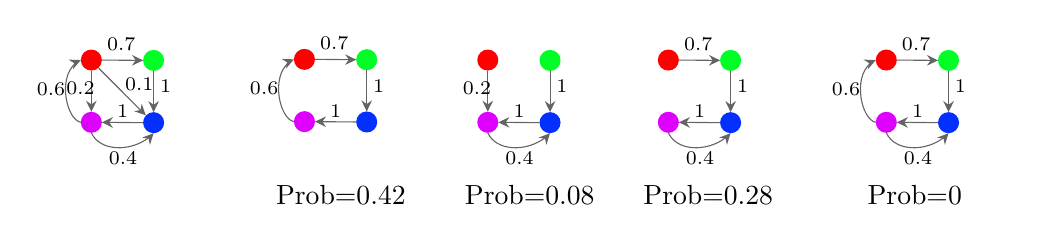
\begin{tikzpicture}[x=0.75pt,y=0.75pt,yscale=-1,xscale=1]
%uncomment if require: \path (0,300); %set diagram left start at 0, and has height of 300

%Shape: Circle [id:dp6680159379724935] 
\draw  [draw opacity=0][fill={rgb, 255:red, 255; green, 0; blue, 0 }  ,fill opacity=1 ] (210,135.27) .. controls (210,132.47) and (212.27,130.2) .. (215.07,130.2) .. controls (217.86,130.2) and (220.13,132.47) .. (220.13,135.27) .. controls (220.13,138.06) and (217.86,140.33) .. (215.07,140.33) .. controls (212.27,140.33) and (210,138.06) .. (210,135.27) -- cycle ;
%Shape: Circle [id:dp2937575833870516] 
\draw  [draw opacity=0][fill={rgb, 255:red, 0; green, 255; blue, 38 }  ,fill opacity=1 ] (240,135.43) .. controls (240,132.64) and (242.27,130.37) .. (245.07,130.37) .. controls (247.86,130.37) and (250.13,132.64) .. (250.13,135.43) .. controls (250.13,138.23) and (247.86,140.5) .. (245.07,140.5) .. controls (242.27,140.5) and (240,138.23) .. (240,135.43) -- cycle ;
%Shape: Circle [id:dp5400820274117357] 
\draw  [draw opacity=0][fill={rgb, 255:red, 3; green, 47; blue, 255 }  ,fill opacity=1 ] (240,165.43) .. controls (240,162.64) and (242.27,160.37) .. (245.07,160.37) .. controls (247.86,160.37) and (250.13,162.64) .. (250.13,165.43) .. controls (250.13,168.23) and (247.86,170.5) .. (245.07,170.5) .. controls (242.27,170.5) and (240,168.23) .. (240,165.43) -- cycle ;
%Shape: Circle [id:dp012766690091095434] 
\draw  [draw opacity=0][fill={rgb, 255:red, 222; green, 0; blue, 255 }  ,fill opacity=1 ] (210,165.27) .. controls (210,162.47) and (212.27,160.2) .. (215.07,160.2) .. controls (217.86,160.2) and (220.13,162.47) .. (220.13,165.27) .. controls (220.13,168.06) and (217.86,170.33) .. (215.07,170.33) .. controls (212.27,170.33) and (210,168.06) .. (210,165.27) -- cycle ;
%Straight Lines [id:da5536414406911649] 
\draw [color={rgb, 255:red, 100; green, 100; blue, 100 }  ,draw opacity=1 ]   (220.13,135.27) -- (237,135.41) ;
\draw [shift={(240,135.43)}, rotate = 180.48] [fill={rgb, 255:red, 100; green, 100; blue, 100 }  ,fill opacity=1 ][line width=0.08]  [draw opacity=0] (5.36,-2.57) -- (0,0) -- (5.36,2.57) -- (3.56,0) -- cycle    ;
%Straight Lines [id:da8056930605061887] 
\draw [color={rgb, 255:red, 100; green, 100; blue, 100 }  ,draw opacity=1 ]   (223.13,165.29) -- (240,165.43) ;
\draw [shift={(220.13,165.27)}, rotate = 0.48] [fill={rgb, 255:red, 100; green, 100; blue, 100 }  ,fill opacity=1 ][line width=0.08]  [draw opacity=0] (5.36,-2.57) -- (0,0) -- (5.36,2.57) -- (3.56,0) -- cycle    ;
%Straight Lines [id:da5796955635821128] 
\draw [color={rgb, 255:red, 100; green, 100; blue, 100 }  ,draw opacity=1 ]   (215.07,140.33) -- (215.07,157.2) ;
\draw [shift={(215.07,160.2)}, rotate = 270] [fill={rgb, 255:red, 100; green, 100; blue, 100 }  ,fill opacity=1 ][line width=0.08]  [draw opacity=0] (5.36,-2.57) -- (0,0) -- (5.36,2.57) -- (3.56,0) -- cycle    ;
%Straight Lines [id:da788839051424455] 
\draw [color={rgb, 255:red, 100; green, 100; blue, 100 }  ,draw opacity=1 ]   (245.07,140.5) -- (245.07,157.37) ;
\draw [shift={(245.07,160.37)}, rotate = 270] [fill={rgb, 255:red, 100; green, 100; blue, 100 }  ,fill opacity=1 ][line width=0.08]  [draw opacity=0] (5.36,-2.57) -- (0,0) -- (5.36,2.57) -- (3.56,0) -- cycle    ;
%Straight Lines [id:da09644761921540357] 
\draw [color={rgb, 255:red, 100; green, 100; blue, 100 }  ,draw opacity=1 ]   (218.63,139.22) -- (239.15,159.76) ;
\draw [shift={(241.27,161.88)}, rotate = 225.04] [fill={rgb, 255:red, 100; green, 100; blue, 100 }  ,fill opacity=1 ][line width=0.08]  [draw opacity=0] (5.36,-2.57) -- (0,0) -- (5.36,2.57) -- (3.56,0) -- cycle    ;
%Curve Lines [id:da6909993804639241] 
\draw [color={rgb, 255:red, 100; green, 100; blue, 100 }  ,draw opacity=1 ]   (207.42,136.86) .. controls (198.7,144.14) and (203.19,163.99) .. (210,165.27) ;
\draw [shift={(210,135.27)}, rotate = 156.35] [fill={rgb, 255:red, 100; green, 100; blue, 100 }  ,fill opacity=1 ][line width=0.08]  [draw opacity=0] (5.36,-2.57) -- (0,0) -- (5.36,2.57) -- (3.56,0) -- cycle    ;
%Curve Lines [id:da43617986234567363] 
\draw [color={rgb, 255:red, 100; green, 100; blue, 100 }  ,draw opacity=1 ]   (215.07,170.33) .. controls (219.24,179.43) and (233.96,179.59) .. (242.88,172.51) ;
\draw [shift={(245.07,170.5)}, rotate = 133.09] [fill={rgb, 255:red, 100; green, 100; blue, 100 }  ,fill opacity=1 ][line width=0.08]  [draw opacity=0] (5.36,-2.57) -- (0,0) -- (5.36,2.57) -- (3.56,0) -- cycle    ;
%Shape: Circle [id:dp9613652888659034] 
\draw  [draw opacity=0][fill={rgb, 255:red, 255; green, 0; blue, 0 }  ,fill opacity=1 ] (312.67,134.93) .. controls (312.67,132.14) and (314.94,129.87) .. (317.73,129.87) .. controls (320.53,129.87) and (322.8,132.14) .. (322.8,134.93) .. controls (322.8,137.73) and (320.53,140) .. (317.73,140) .. controls (314.94,140) and (312.67,137.73) .. (312.67,134.93) -- cycle ;
%Shape: Circle [id:dp4333461787824253] 
\draw  [draw opacity=0][fill={rgb, 255:red, 0; green, 255; blue, 38 }  ,fill opacity=1 ] (342.67,135.1) .. controls (342.67,132.3) and (344.94,130.03) .. (347.73,130.03) .. controls (350.53,130.03) and (352.8,132.3) .. (352.8,135.1) .. controls (352.8,137.9) and (350.53,140.17) .. (347.73,140.17) .. controls (344.94,140.17) and (342.67,137.9) .. (342.67,135.1) -- cycle ;
%Shape: Circle [id:dp03365070392980951] 
\draw  [draw opacity=0][fill={rgb, 255:red, 3; green, 47; blue, 255 }  ,fill opacity=1 ] (342.67,165.1) .. controls (342.67,162.3) and (344.94,160.03) .. (347.73,160.03) .. controls (350.53,160.03) and (352.8,162.3) .. (352.8,165.1) .. controls (352.8,167.9) and (350.53,170.17) .. (347.73,170.17) .. controls (344.94,170.17) and (342.67,167.9) .. (342.67,165.1) -- cycle ;
%Shape: Circle [id:dp9062547154952614] 
\draw  [draw opacity=0][fill={rgb, 255:red, 222; green, 0; blue, 255 }  ,fill opacity=1 ] (312.67,164.93) .. controls (312.67,162.14) and (314.94,159.87) .. (317.73,159.87) .. controls (320.53,159.87) and (322.8,162.14) .. (322.8,164.93) .. controls (322.8,167.73) and (320.53,170) .. (317.73,170) .. controls (314.94,170) and (312.67,167.73) .. (312.67,164.93) -- cycle ;
%Straight Lines [id:da5461621784127331] 
\draw [color={rgb, 255:red, 100; green, 100; blue, 100 }  ,draw opacity=1 ]   (322.8,134.93) -- (339.67,135.07) ;
\draw [shift={(342.67,135.1)}, rotate = 180.48] [fill={rgb, 255:red, 100; green, 100; blue, 100 }  ,fill opacity=1 ][line width=0.08]  [draw opacity=0] (5.36,-2.57) -- (0,0) -- (5.36,2.57) -- (3.56,0) -- cycle    ;
%Straight Lines [id:da09616201897578192] 
\draw [color={rgb, 255:red, 100; green, 100; blue, 100 }  ,draw opacity=1 ]   (325.8,164.96) -- (342.67,165.1) ;
\draw [shift={(322.8,164.93)}, rotate = 0.48] [fill={rgb, 255:red, 100; green, 100; blue, 100 }  ,fill opacity=1 ][line width=0.08]  [draw opacity=0] (5.36,-2.57) -- (0,0) -- (5.36,2.57) -- (3.56,0) -- cycle    ;
%Straight Lines [id:da5502296583487012] 
\draw [color={rgb, 255:red, 100; green, 100; blue, 100 }  ,draw opacity=1 ]   (347.73,140.17) -- (347.73,157.03) ;
\draw [shift={(347.73,160.03)}, rotate = 270] [fill={rgb, 255:red, 100; green, 100; blue, 100 }  ,fill opacity=1 ][line width=0.08]  [draw opacity=0] (5.36,-2.57) -- (0,0) -- (5.36,2.57) -- (3.56,0) -- cycle    ;
%Curve Lines [id:da23324631718484024] 
\draw [color={rgb, 255:red, 100; green, 100; blue, 100 }  ,draw opacity=1 ]   (310.09,136.53) .. controls (301.37,143.81) and (305.86,163.66) .. (312.67,164.93) ;
\draw [shift={(312.67,134.93)}, rotate = 156.35] [fill={rgb, 255:red, 100; green, 100; blue, 100 }  ,fill opacity=1 ][line width=0.08]  [draw opacity=0] (5.36,-2.57) -- (0,0) -- (5.36,2.57) -- (3.56,0) -- cycle    ;
%Shape: Circle [id:dp6818622582337936] 
\draw  [draw opacity=0][fill={rgb, 255:red, 255; green, 0; blue, 0 }  ,fill opacity=1 ] (401,135.27) .. controls (401,132.47) and (403.27,130.2) .. (406.07,130.2) .. controls (408.86,130.2) and (411.13,132.47) .. (411.13,135.27) .. controls (411.13,138.06) and (408.86,140.33) .. (406.07,140.33) .. controls (403.27,140.33) and (401,138.06) .. (401,135.27) -- cycle ;
%Shape: Circle [id:dp06363585140660888] 
\draw  [draw opacity=0][fill={rgb, 255:red, 0; green, 255; blue, 38 }  ,fill opacity=1 ] (431,135.43) .. controls (431,132.64) and (433.27,130.37) .. (436.07,130.37) .. controls (438.86,130.37) and (441.13,132.64) .. (441.13,135.43) .. controls (441.13,138.23) and (438.86,140.5) .. (436.07,140.5) .. controls (433.27,140.5) and (431,138.23) .. (431,135.43) -- cycle ;
%Shape: Circle [id:dp6515401713841082] 
\draw  [draw opacity=0][fill={rgb, 255:red, 3; green, 47; blue, 255 }  ,fill opacity=1 ] (431,165.43) .. controls (431,162.64) and (433.27,160.37) .. (436.07,160.37) .. controls (438.86,160.37) and (441.13,162.64) .. (441.13,165.43) .. controls (441.13,168.23) and (438.86,170.5) .. (436.07,170.5) .. controls (433.27,170.5) and (431,168.23) .. (431,165.43) -- cycle ;
%Shape: Circle [id:dp8403565146161891] 
\draw  [draw opacity=0][fill={rgb, 255:red, 222; green, 0; blue, 255 }  ,fill opacity=1 ] (401,165.27) .. controls (401,162.47) and (403.27,160.2) .. (406.07,160.2) .. controls (408.86,160.2) and (411.13,162.47) .. (411.13,165.27) .. controls (411.13,168.06) and (408.86,170.33) .. (406.07,170.33) .. controls (403.27,170.33) and (401,168.06) .. (401,165.27) -- cycle ;
%Straight Lines [id:da37129508524849975] 
\draw [color={rgb, 255:red, 100; green, 100; blue, 100 }  ,draw opacity=1 ]   (414.13,165.29) -- (431,165.43) ;
\draw [shift={(411.13,165.27)}, rotate = 0.48] [fill={rgb, 255:red, 100; green, 100; blue, 100 }  ,fill opacity=1 ][line width=0.08]  [draw opacity=0] (5.36,-2.57) -- (0,0) -- (5.36,2.57) -- (3.56,0) -- cycle    ;
%Straight Lines [id:da7145815190421096] 
\draw [color={rgb, 255:red, 100; green, 100; blue, 100 }  ,draw opacity=1 ]   (406.07,140.33) -- (406.07,157.2) ;
\draw [shift={(406.07,160.2)}, rotate = 270] [fill={rgb, 255:red, 100; green, 100; blue, 100 }  ,fill opacity=1 ][line width=0.08]  [draw opacity=0] (5.36,-2.57) -- (0,0) -- (5.36,2.57) -- (3.56,0) -- cycle    ;
%Straight Lines [id:da39415211091672386] 
\draw [color={rgb, 255:red, 100; green, 100; blue, 100 }  ,draw opacity=1 ]   (436.07,140.5) -- (436.07,157.37) ;
\draw [shift={(436.07,160.37)}, rotate = 270] [fill={rgb, 255:red, 100; green, 100; blue, 100 }  ,fill opacity=1 ][line width=0.08]  [draw opacity=0] (5.36,-2.57) -- (0,0) -- (5.36,2.57) -- (3.56,0) -- cycle    ;
%Curve Lines [id:da9757843179704913] 
\draw [color={rgb, 255:red, 100; green, 100; blue, 100 }  ,draw opacity=1 ]   (406.07,170.33) .. controls (410.24,179.43) and (424.96,179.59) .. (433.88,172.51) ;
\draw [shift={(436.07,170.5)}, rotate = 133.09] [fill={rgb, 255:red, 100; green, 100; blue, 100 }  ,fill opacity=1 ][line width=0.08]  [draw opacity=0] (5.36,-2.57) -- (0,0) -- (5.36,2.57) -- (3.56,0) -- cycle    ;
%Shape: Circle [id:dp04380357617227837] 
\draw  [draw opacity=0][fill={rgb, 255:red, 255; green, 0; blue, 0 }  ,fill opacity=1 ] (488,135.27) .. controls (488,132.47) and (490.27,130.2) .. (493.07,130.2) .. controls (495.86,130.2) and (498.13,132.47) .. (498.13,135.27) .. controls (498.13,138.06) and (495.86,140.33) .. (493.07,140.33) .. controls (490.27,140.33) and (488,138.06) .. (488,135.27) -- cycle ;
%Shape: Circle [id:dp29949986935781037] 
\draw  [draw opacity=0][fill={rgb, 255:red, 0; green, 255; blue, 38 }  ,fill opacity=1 ] (518,135.43) .. controls (518,132.64) and (520.27,130.37) .. (523.07,130.37) .. controls (525.86,130.37) and (528.13,132.64) .. (528.13,135.43) .. controls (528.13,138.23) and (525.86,140.5) .. (523.07,140.5) .. controls (520.27,140.5) and (518,138.23) .. (518,135.43) -- cycle ;
%Shape: Circle [id:dp5511672247736801] 
\draw  [draw opacity=0][fill={rgb, 255:red, 3; green, 47; blue, 255 }  ,fill opacity=1 ] (518,165.43) .. controls (518,162.64) and (520.27,160.37) .. (523.07,160.37) .. controls (525.86,160.37) and (528.13,162.64) .. (528.13,165.43) .. controls (528.13,168.23) and (525.86,170.5) .. (523.07,170.5) .. controls (520.27,170.5) and (518,168.23) .. (518,165.43) -- cycle ;
%Shape: Circle [id:dp9769153872658556] 
\draw  [draw opacity=0][fill={rgb, 255:red, 222; green, 0; blue, 255 }  ,fill opacity=1 ] (488,165.27) .. controls (488,162.47) and (490.27,160.2) .. (493.07,160.2) .. controls (495.86,160.2) and (498.13,162.47) .. (498.13,165.27) .. controls (498.13,168.06) and (495.86,170.33) .. (493.07,170.33) .. controls (490.27,170.33) and (488,168.06) .. (488,165.27) -- cycle ;
%Straight Lines [id:da5613131489306487] 
\draw [color={rgb, 255:red, 100; green, 100; blue, 100 }  ,draw opacity=1 ]   (498.13,135.27) -- (515,135.41) ;
\draw [shift={(518,135.43)}, rotate = 180.48] [fill={rgb, 255:red, 100; green, 100; blue, 100 }  ,fill opacity=1 ][line width=0.08]  [draw opacity=0] (5.36,-2.57) -- (0,0) -- (5.36,2.57) -- (3.56,0) -- cycle    ;
%Straight Lines [id:da005025679675679795] 
\draw [color={rgb, 255:red, 100; green, 100; blue, 100 }  ,draw opacity=1 ]   (501.13,165.29) -- (518,165.43) ;
\draw [shift={(498.13,165.27)}, rotate = 0.48] [fill={rgb, 255:red, 100; green, 100; blue, 100 }  ,fill opacity=1 ][line width=0.08]  [draw opacity=0] (5.36,-2.57) -- (0,0) -- (5.36,2.57) -- (3.56,0) -- cycle    ;
%Straight Lines [id:da1558253629861852] 
\draw [color={rgb, 255:red, 100; green, 100; blue, 100 }  ,draw opacity=1 ]   (523.07,140.5) -- (523.07,157.37) ;
\draw [shift={(523.07,160.37)}, rotate = 270] [fill={rgb, 255:red, 100; green, 100; blue, 100 }  ,fill opacity=1 ][line width=0.08]  [draw opacity=0] (5.36,-2.57) -- (0,0) -- (5.36,2.57) -- (3.56,0) -- cycle    ;
%Curve Lines [id:da36403543815313033] 
\draw [color={rgb, 255:red, 100; green, 100; blue, 100 }  ,draw opacity=1 ]   (493.07,170.33) .. controls (497.24,179.43) and (511.96,179.59) .. (520.88,172.51) ;
\draw [shift={(523.07,170.5)}, rotate = 133.09] [fill={rgb, 255:red, 100; green, 100; blue, 100 }  ,fill opacity=1 ][line width=0.08]  [draw opacity=0] (5.36,-2.57) -- (0,0) -- (5.36,2.57) -- (3.56,0) -- cycle    ;
%Shape: Circle [id:dp32223667430392] 
\draw  [draw opacity=0][fill={rgb, 255:red, 255; green, 0; blue, 0 }  ,fill opacity=1 ] (593,135.27) .. controls (593,132.47) and (595.27,130.2) .. (598.07,130.2) .. controls (600.86,130.2) and (603.13,132.47) .. (603.13,135.27) .. controls (603.13,138.06) and (600.86,140.33) .. (598.07,140.33) .. controls (595.27,140.33) and (593,138.06) .. (593,135.27) -- cycle ;
%Shape: Circle [id:dp5630106243065429] 
\draw  [draw opacity=0][fill={rgb, 255:red, 0; green, 255; blue, 38 }  ,fill opacity=1 ] (623,135.43) .. controls (623,132.64) and (625.27,130.37) .. (628.07,130.37) .. controls (630.86,130.37) and (633.13,132.64) .. (633.13,135.43) .. controls (633.13,138.23) and (630.86,140.5) .. (628.07,140.5) .. controls (625.27,140.5) and (623,138.23) .. (623,135.43) -- cycle ;
%Shape: Circle [id:dp7466122496388676] 
\draw  [draw opacity=0][fill={rgb, 255:red, 3; green, 47; blue, 255 }  ,fill opacity=1 ] (623,165.43) .. controls (623,162.64) and (625.27,160.37) .. (628.07,160.37) .. controls (630.86,160.37) and (633.13,162.64) .. (633.13,165.43) .. controls (633.13,168.23) and (630.86,170.5) .. (628.07,170.5) .. controls (625.27,170.5) and (623,168.23) .. (623,165.43) -- cycle ;
%Shape: Circle [id:dp031700867746790706] 
\draw  [draw opacity=0][fill={rgb, 255:red, 222; green, 0; blue, 255 }  ,fill opacity=1 ] (593,165.27) .. controls (593,162.47) and (595.27,160.2) .. (598.07,160.2) .. controls (600.86,160.2) and (603.13,162.47) .. (603.13,165.27) .. controls (603.13,168.06) and (600.86,170.33) .. (598.07,170.33) .. controls (595.27,170.33) and (593,168.06) .. (593,165.27) -- cycle ;
%Straight Lines [id:da674567593051244] 
\draw [color={rgb, 255:red, 100; green, 100; blue, 100 }  ,draw opacity=1 ]   (603.13,135.27) -- (620,135.41) ;
\draw [shift={(623,135.43)}, rotate = 180.48] [fill={rgb, 255:red, 100; green, 100; blue, 100 }  ,fill opacity=1 ][line width=0.08]  [draw opacity=0] (5.36,-2.57) -- (0,0) -- (5.36,2.57) -- (3.56,0) -- cycle    ;
%Straight Lines [id:da19529599944373754] 
\draw [color={rgb, 255:red, 100; green, 100; blue, 100 }  ,draw opacity=1 ]   (606.13,165.29) -- (623,165.43) ;
\draw [shift={(603.13,165.27)}, rotate = 0.48] [fill={rgb, 255:red, 100; green, 100; blue, 100 }  ,fill opacity=1 ][line width=0.08]  [draw opacity=0] (5.36,-2.57) -- (0,0) -- (5.36,2.57) -- (3.56,0) -- cycle    ;
%Straight Lines [id:da00219011682676884] 
\draw [color={rgb, 255:red, 100; green, 100; blue, 100 }  ,draw opacity=1 ]   (628.07,140.5) -- (628.07,157.37) ;
\draw [shift={(628.07,160.37)}, rotate = 270] [fill={rgb, 255:red, 100; green, 100; blue, 100 }  ,fill opacity=1 ][line width=0.08]  [draw opacity=0] (5.36,-2.57) -- (0,0) -- (5.36,2.57) -- (3.56,0) -- cycle    ;
%Curve Lines [id:da28811211023069117] 
\draw [color={rgb, 255:red, 100; green, 100; blue, 100 }  ,draw opacity=1 ]   (590.42,136.86) .. controls (581.7,144.14) and (586.19,163.99) .. (593,165.27) ;
\draw [shift={(593,135.27)}, rotate = 156.35] [fill={rgb, 255:red, 100; green, 100; blue, 100 }  ,fill opacity=1 ][line width=0.08]  [draw opacity=0] (5.36,-2.57) -- (0,0) -- (5.36,2.57) -- (3.56,0) -- cycle    ;
%Curve Lines [id:da1762071401291876] 
\draw [color={rgb, 255:red, 100; green, 100; blue, 100 }  ,draw opacity=1 ]   (598.07,170.33) .. controls (602.24,179.43) and (616.96,179.59) .. (625.88,172.51) ;
\draw [shift={(628.07,170.5)}, rotate = 133.09] [fill={rgb, 255:red, 100; green, 100; blue, 100 }  ,fill opacity=1 ][line width=0.08]  [draw opacity=0] (5.36,-2.57) -- (0,0) -- (5.36,2.57) -- (3.56,0) -- cycle    ;

% Text Node
\draw (233.3,127.45) node  [font=\scriptsize] [align=left] {\begin{minipage}[lt]{16pt}\setlength\topsep{0pt}
0.7
\end{minipage}};
% Text Node
\draw (258.83,148.05) node  [font=\scriptsize] [align=left] {\begin{minipage}[lt]{16pt}\setlength\topsep{0pt}
1
\end{minipage}};
% Text Node
\draw (242.03,146.75) node  [font=\scriptsize] [align=left] {\begin{minipage}[lt]{16pt}\setlength\topsep{0pt}
0.1
\end{minipage}};
% Text Node
\draw (213.7,148.75) node  [font=\scriptsize] [align=left] {\begin{minipage}[lt]{16pt}\setlength\topsep{0pt}
0.2
\end{minipage}};
% Text Node
\draw (238.17,160.05) node  [font=\scriptsize] [align=left] {\begin{minipage}[lt]{16pt}\setlength\topsep{0pt}
1
\end{minipage}};
% Text Node
\draw (234.17,182.72) node  [font=\scriptsize] [align=left] {\begin{minipage}[lt]{16pt}\setlength\topsep{0pt}
0.4
\end{minipage}};
% Text Node
\draw (199.5,149.38) node  [font=\scriptsize] [align=left] {\begin{minipage}[lt]{16pt}\setlength\topsep{0pt}
0.6
\end{minipage}};

% Text Node
\draw (335.97,127.12) node  [font=\scriptsize] [align=left] {\begin{minipage}[lt]{16pt}\setlength\topsep{0pt}
0.7
\end{minipage}};
% Text Node
\draw (361.5,147.72) node  [font=\scriptsize] [align=left] {\begin{minipage}[lt]{16pt}\setlength\topsep{0pt}
1
\end{minipage}};
% Text Node
\draw (340.83,159.72) node  [font=\scriptsize] [align=left] {\begin{minipage}[lt]{16pt}\setlength\topsep{0pt}
1
\end{minipage}};
% Text Node
\draw (302.17,149.05) node  [font=\scriptsize] [align=left] {\begin{minipage}[lt]{16pt}\setlength\topsep{0pt}
0.6
\end{minipage}};
% Text Node
\draw (449.83,148.05) node  [font=\scriptsize] [align=left] {\begin{minipage}[lt]{16pt}\setlength\topsep{0pt}
1
\end{minipage}};
% Text Node
\draw (404.7,148.75) node  [font=\scriptsize] [align=left] {\begin{minipage}[lt]{16pt}\setlength\topsep{0pt}
0.2
\end{minipage}};
% Text Node
\draw (429.17,160.05) node  [font=\scriptsize] [align=left] {\begin{minipage}[lt]{16pt}\setlength\topsep{0pt}
1
\end{minipage}};
% Text Node
\draw (425.17,182.72) node  [font=\scriptsize] [align=left] {\begin{minipage}[lt]{16pt}\setlength\topsep{0pt}
0.4
\end{minipage}};
% Text Node
\draw (511.3,127.45) node  [font=\scriptsize] [align=left] {\begin{minipage}[lt]{16pt}\setlength\topsep{0pt}
0.7
\end{minipage}};
% Text Node
\draw (536.83,148.05) node  [font=\scriptsize] [align=left] {\begin{minipage}[lt]{16pt}\setlength\topsep{0pt}
1
\end{minipage}};
% Text Node
\draw (516.17,160.05) node  [font=\scriptsize] [align=left] {\begin{minipage}[lt]{16pt}\setlength\topsep{0pt}
1
\end{minipage}};
% Text Node
\draw (512.17,182.72) node  [font=\scriptsize] [align=left] {\begin{minipage}[lt]{16pt}\setlength\topsep{0pt}
0.4
\end{minipage}};
% Text Node
\draw (616.3,127.45) node  [font=\scriptsize] [align=left] {\begin{minipage}[lt]{16pt}\setlength\topsep{0pt}
0.7
\end{minipage}};
% Text Node
\draw (641.83,148.05) node  [font=\scriptsize] [align=left] {\begin{minipage}[lt]{16pt}\setlength\topsep{0pt}
1
\end{minipage}};
% Text Node
\draw (621.17,160.05) node  [font=\scriptsize] [align=left] {\begin{minipage}[lt]{16pt}\setlength\topsep{0pt}
1
\end{minipage}};
% Text Node
\draw (617.17,182.72) node  [font=\scriptsize] [align=left] {\begin{minipage}[lt]{16pt}\setlength\topsep{0pt}
0.4
\end{minipage}};
% Text Node
\draw (582.5,149.38) node  [font=\scriptsize] [align=left] {\begin{minipage}[lt]{16pt}\setlength\topsep{0pt}
0.6
\end{minipage}};

% Text Node
\draw (237.57,200) node   [align=left] {\begin{minipage}[lt]{20.9pt}\setlength\topsep{0pt}
$\bfpi$
\end{minipage}};


% Text Node
\draw (318,200) node   [align=left] {\begin{minipage}[lt]{20.9pt}\setlength\topsep{0pt}
Prob=0.42
\end{minipage}};


\draw (409,200) node   [align=left] {\begin{minipage}[lt]{20.9pt}\setlength\topsep{0pt}
Prob=0.08
\end{minipage}};


% Text Node
\draw (495,200) node   [align=left] {\begin{minipage}[lt]{20.9pt}\setlength\topsep{0pt}
Prob=0.28
\end{minipage}};

% Text Node
\draw (603,200) node   [align=left] {\begin{minipage}[lt]{20.9pt}\setlength\topsep{0pt}
Prob=0
\end{minipage}};

\end{tikzpicture}

\section{Background}


In this section, we introduce a set of relevant concepts in quantum computing,
% that are  to our work, 
including the building block of quantum computing, the properties of the qubit, and the quantum state of the qubit. 

\def\Zero{
\begin{bmatrix}
    1 \\
    0 \\
\end{bmatrix}}

\def\One{
\begin{bmatrix}
    0 \\
    1 \\
\end{bmatrix}}

\def\sv{
\begin{bmatrix}
    \alpha \\
    \beta \\
\end{bmatrix}}

\def\svcomplex{
\begin{bmatrix}
    a+bi \\
    c+di \\
\end{bmatrix}}


\subsection{Building Block of Quantum Computing}

\textbf{Qubit},
the quantum version of the classic bit, is the basic unit in quantum computing. Similar to a classical bit, there are two computational basis states called state 0 and state 1 for a qubit~\cite{ciaran2021qc4c}. 
However, 
% in contrast to a classical bit, which is either in state 
% 0 or state 1, 
a qubit can also be in an arbitrary linear superposition of state 0 and state 1~\cite{ciaran2021qc4c, rieffel2000introQCnonP}, which is well-known as quantum superposition.
Mathematically, one can represent a qubit using the form of a state vector~\cite{rieffel2000introQCnonP}.
% Bra-Ket Notation or Bloch sphere. 
% Kets like $\ket{x}$ denote column vectors and are typically used to describe quantum states~\cite{rieffel2000introQCnonP}. 
% For instance, state 0 and state 1 can be expressed as $\ket{0}$ = $\Zero$, $\ket{1}$ = $\One$, respectively. 
% When dealing with qubits, and quantum computing in general, a fixed basis with respect to which all statements are made has been chosen in advance. In particular, unless otherwise specified, all measurements will be made concerning the standard basis for quantum computing, ${\ket{0}, \ket{1}}$~\cite{rieffel2000introQCnonP}. 
% As mentioned above, the quantum state $\ket{\psi}$ of a qubit can also be represented in a linear superposition of $\ket{0}$ and $\ket{1}$. 
% Section \ref{qubit_prop} includes more details about the concept of superposition. 

% The state of a single qubit can also be studied by Bloch Sphere. Bloch Sphere is a visual representation of a qubit with similar geometric properties to the unit circle from trigonometry. 
% % Each point on Bloch Sphere corresponds to a different possible superposition of a single qubit~\cite{ciaran2021qc4c}. The top and bottom of the Bloch Sphere correspond to the two measurable quantum states of the qubit, $\ket{0}$ and $\ket{1}$~\cite{ciaran2021qc4c}.
% A vector on the Bloch Sphere, which can point to any of the different locations on the surface of the sphere, indicates the current quantum state of the qubit~\cite{ciaran2021qc4c}. Figure \ref{fig:1}\component{A} is an example of Bloch Sphere visualizing the quantum state of a single qubit. Bloch Sphere is a helpful visualization for understanding how a qubit can have infinite possible quantum states. However, it can only represent one qubit and does not work for systems of two or more qubits~\cite{ciaran2021qc4c, bardin2021microwaves, wie2014bloch}.


% quantum state, superposition, |0>, |1>, psi-matrix, denoted by |0>
% quantum state is represented by |psi>
% similar to classical bit, |0>, |1>
% unlike classical bit, a|0> + b|1>, will discuss this in section 3.2. |psi> = a|0> + b|1> = a[1,0] + b[0,1] = [a,b]


\textbf{Quantum gate},
just like the manipulation of classical bits using classical logic instructions such as \textit{OR} and \textit{AND}, it is applied to qubits to change their quantum states. 
% and the quantum states of qubits change depending on which gate is applied. 
% In Bloch Sphere representation, gates provide instructions for rotating the qubit’s vector around the sphere~\cite{ciaran2021qc4c}. 
Mathematically, quantum gates are represented as operation matrices, acting on single qubit or multiple qubits.
Operations of quantum gates are equivalent to the dot products with the state vector of qubits.
% \yong{Applying xxx to qubits? Please double check the verb.}
% that act on qubits using matrix multiplication.
%Quantum Gate are represented by matrix. Single quantum gate like H, Multiple Quantum gate like CNOT.
%Pics of gate

\textbf{Quantum circuit},
similar to the classical circuit, is the implementation of the quantum program for execution.
A quantum circuit consists of a set of quantum gates, acting on one or multiple fixed qubits.
% in a quantum computer or quantum simulator.
As shown in Figure \ref{fig:case1} and \ref{fig:case2}, a quantum state will be initialized from the start of the quantum circuit and manipulated by quantum gates designed in the quantum circuit. 
% The final execution result is retrieved by measuring each quantum state.




\subsection{Properties of Qubit}
\label{qubit_prop}
\textbf{Superposition}
indicates that a qubit can not only be in one of the computational basis states $\ket{0}$ or $\ket{1}$, but also in a linear superposition of this two states~\cite {nara1999QC4B}.
% As mentioned in Section 3.1, compared with classical bits, the value can only be either 0 or 1, 
Thus, the quantum state $\ket{\psi}$ of a qubit is described by $\alpha\ket{0} + \beta\ket{1}$, where the complex numbers $\alpha$ and $\beta$ are called \textit{amplitudes} such that $|\alpha|^2 + |\beta|^2 = 1$~\cite{rieffel2000introQCnonP}. 
Meanwhile, 
% Once such superposition is measured with respect to the basis state {$\ket{0}$ and $\ket{1}$}, 
the probability of measuring $\ket{0}$ is $|\alpha|^2$ and the probability of $\ket{1}$ is $|\beta|^2$
~\cite{ciaran2021qc4c, rieffel2000introQCnonP,nara1999QC4B}.
% The real power of quantum computing derives from the exponentially increasing state space of multiple qubits,
as a quantum system with $n$ qubits can generate a linear superposition of $2^n$ basis states simultaneously~\cite{rieffel2000introQCnonP, Hey1999QuantumCA}.
% : since the quantum state of a single qubit can be in a linear superposition of $\ket{0}$ and $\ket{1}$, a quantum system with $n$ qubits can generate a linear superposition of $2^n$ basis states~\cite{rieffel2000introQCnonP, Hey1999QuantumCA}. 
% Thus, creating such a superposition is the critical properties of achieving the quantum advantage~\cite{Hey1999QuantumCA}.

% that gives quantum parallel processing its power~\cite{Hey1999QuantumCA}.

% Example.
% It is noteworthy that even though a qubit can have infinitely many superposition states before measurement, measuring a qubit collapses its superposition state into one of two possibilities~\cite{ciaran2021qc4c, rieffel2000introQCnonP}. That is, if the measurement of $\ket{\psi} = \alpha\ket{0} + \beta\ket{1}$ results in $\ket{0}$, then the state changes to $\ket{0}$, and a second measurement with respect to the same basis will return $\ket{0}$ with probability 1~\cite{rieffel2000introQCnonP}. Thus, unless the original state happens to be one of the basis vectors, the measurement will change that state, and it is impossible to determine what the original state was~\cite{rieffel2000introQCnonP}.


\textbf{Entanglement}
is an essential feature that differentiates qubits and classical bits. 
Specifically,
% In quantum computing, 
when two or more qubits are entangled, their quantum states are coupled with each other,
%they will exist in a single quantum state. 
so that changing the quantum state of any one qubit will instantaneously change the other qubit's quantum state in a predictable way~\cite{rieffel2000introQCnonP}.
% Instead, an easy test to determine if a system is entangled or not is to check if measuring the value of one qubit changes the probability distribution of the other qubit~\cite{ciaran2021qc4c}. 
% For instance, the quantum state $\ket{\psi} = \dfrac{1}{\sqrt{2}}\ket{00} + \dfrac{1}{\sqrt{2}}\ket{11}$ is entangled since the probability that the first qubit is measured to be $\ket{0}$ is $1/2$ if the second qubit has not been measured. 
Note that the entanglement operation requires more than one qubit, making it critically important to analyze the quantum states of multiple qubits instead of a single qubit.
% Note that the two-qubit entangle is a specific scenario of two-qubit state, where the two qubits are entangled.
% Thus, the approach of two-qubit state representation is of great value for solving the two-qubit entanglement representation.
% However, if the second qubit has been measured, the probability that the first qubit is measured as $\ket{0}$ is 1 or 0, if the second qubit was measured as $\ket{0}$ or $\ket{1}$, respectively. In this case, the result of measuring the first qubit depends on the measurement of the second qubit. 
% In contrast, in the case of $\ket{\psi} = \dfrac{1}{\sqrt{2}}\ket{00} + \dfrac{1}{\sqrt{2}}\ket{01}$, two qubits are not entangled since any measurement of the first qubit will yield $\ket{0}$ regardless of whether the second qubit was measured. Similarly, the second qubit has a fifty-fifty chance of being measured as $\ket{0}$ regardless of whether the first qubit was measured or not~\cite{rieffel2000introQCnonP}. Entanglement happens even if qubits are far away from each other. When two or more qubits are entangled, the quantum state can not be described in terms of the state of each of its components (qubits) separately. 


\subsection{Quantum State of Qubit}
\label{sec:3.3}
In quantum computing, a quantum state is a mathematical entity that provides a probability distribution of different basis states.
% on a single qubit or multiple qubits. 
For clarity, we start with a single-qubit state, and the case of a two-qubit state will be derived from these results.
In Section \ref{sec:venus}, we will illustrate how we apply the following quantum computing characteristics and encode them with a variety of 2D geometric shapes to form our visual design.

\textbf{Single-qubit state} represents the quantum state for a single qubit.
% From Section 3.1 and 3.2,
Recall that
the quantum state of a qubit can be a superposition of basis states {$\ket{0}$ and $\ket{1}$}, thus the quantum state $\ket{\psi}$ can be expressed as $\ket{\psi} = \alpha\ket{0} + \beta\ket{1} = \alpha\Zero + \beta\One = \sv$, where the amplitudes $\alpha$ and $\beta$ satisfy:
% are complex numbers
% , and $|\alpha|^2 + |\beta|^2 = 1$. 
% and can be calculated as follows:


\begin{equation}
\label{equation:1}
\alpha=a+b\cdot i, \beta=c+d\cdot i,
\end{equation}

where $i$ is the imaginary unit, and $a$, $b$, $c$, and $d$ are real numbers.
% Thus, the quantum state of a single qubit can be expressed as $\ket{\psi} = \sv = \svcomplex$. 
Based on the quantum 
% computing 
theory, the probability of a measured quantum state (\textit{e.g.}, $\ket{0}$) satisfies


\begin{equation}
\label{equation:2_1}
Pr(\ket{0}) = |\alpha|^2 = |a|^2 + |b|^2.
\end{equation}

% By definition, a complex number is a number of the form $a + bi$, where $a$ and $b$ are real numbers, and $i$ is an indeterminate satisfying $i^2=-1$. 
Meanwhile, since the amplitudes satisfy a normalization constraint,\textit{ i.e.}, the sum of the probabilities of the two quantum states for single qubits (\textit{i.e.}, $\ket{0}$ and $\ket{1}$) consistently equals 1, 
thus applying Equation \ref{equation:2_1}  yields


\begin{equation}
\label{equation:4}
|a|^2+|b|^2+|c|^2+|d|^2 = 1.
\end{equation}

% $a$, $b$, $c$ and $d$ satisfy 
% $a^2+b^2+c^2+d^2=1$.


\textbf{Two-qubit state} is the quantum states executing on a pair of qubits,
\modify{which can be calculated by the tensor product of two single-qubit states, \textit{e.g.}, $\ket{00} = \ket{0} \otimes \ket{0}$}.
% \yong{Pls check my comments on Overleaf Review.}
Meanwhile, any two qubits can be in the state $\ket{\psi} = \alpha\ket{00} + \beta\ket{01} + \gamma\ket{10} + \delta\ket{11}$, where the amplitudes $\alpha$, $\beta$, $\gamma$, and $\delta$ satisfy:

% For two-qubit entanglement, the state vector consists of four complex number amplitudes (\textit{i.e.}, $\alpha-$ $\beta-$ $\gamma-$ $\delta-$components), which can be represented as follows:


\begin{equation}
\label{equation:5}
\begin{aligned}
\alpha = a + b \cdot i, \beta = c + d \cdot i,\\
\gamma = e + f \cdot i, \delta = g + h \cdot i.
%  &\quad
\end{aligned}
\end{equation}



Similar to single-qubit states, since the probabilities of all possible qubits equal 1, the four amplitudes satisfy  $|\alpha|^2 + |\beta|^2 + |\gamma|^2 + |\delta|^2 = 1$. 
By applying Equation \ref{equation:5} to the above constraint,
we have
% By applying Equation \ref{equation:5} to Equation \ref{equation:6}, we can calculate the lengths of all line segments for state vector display as follows:


\begin{equation}
\label{equation:7}
|a|^2+|b|^2+|c|^2+|d|^2+|e|^2+|f|^2+|g|^2+|h|^2 = 1.
\end{equation}



% \begin{figure}[t]
% \centering 
% \includegraphics[width=0.7\linewidth]{figures/1_.pdf}
% \caption{A widely-used visualization called Bloch Sphere for quantum state representation.
% % (B) The workflow of the co-design process with domain experts. The steps connected by the green line indicate the stage of the preliminary interview for the initial prototype, while those steps connected by the blue line represent the iterative tuning process in the stage of the expert test.
% }
% \label{fig:1}
% \end{figure}


\documentclass[letterpaper, 12pt, journal, twoside]{support/IEEEtran}
\usepackage[fleqn]{amsmath}
\usepackage{times}
\usepackage[pdftex]{graphicx}
\usepackage{subfigure}
\usepackage{amsmath,amssymb,amsopn,amstext,amsfonts}
\usepackage{cancel}
\usepackage[noadjust]{cite}
\usepackage{soul}
\usepackage{caption}
\captionsetup{font={small}}

\captionsetup[figure]{labelfont={},textfont={}}


\usepackage{balance}
\usepackage{color}
\usepackage{mathtools}
% \usepackage{algorithm}
% \usepackage{algorithmic}
\usepackage{bm}
%\newtheorem{theorem}{Theorem}
\usepackage{ diagbox}
\usepackage{float}
\usepackage{epstopdf}
\usepackage{url}
\usepackage{multirow}
\usepackage{tikz}
\usepackage{subeqnarray}
\usepackage{cases}
\usepackage{booktabs}
\usepackage[linkcolor=black,citecolor=black,urlcolor=black,colorlinks=true]{hyperref}
\usepackage{algorithm}
\usepackage[noend]{algpseudocode}
\newtheorem{myTheo}{Theorem}
%\newtheorem{thm}{Theorem}[section] %如果不采用章节号做前缀,则不用[section]
\newtheorem{myDef}{Definition} %这句定义使得defn环境和thm共享编号
\newtheorem{lemma}{Lemma} %这句定义使得lem环境和thm共享编号
\newtheorem{myCollo}{Corollary}
\newtheorem{remark}{Remark}
%\newtheorem{lemma}{Lemma}
\newtheorem{myPro}{Proposition}
\newtheorem{assumption}{Assumption}
\newtheorem{example}{Example}
\soulregister\cite7
\soulregister\citep7
\soulregister\citet7
\soulregister\ref7
\soulregister\it7
\soulregister\pageref7

\bibliographystyle{support/IEEEtran}

\newcommand\px{\mathrel{/\mkern-5mu/}}  %平行
\newcommand{\ann}[1]{%
    \begin{tikzpicture}[remember picture, baseline=-0.75ex]%
        \node[coordinate] (inText) {};%
    \end{tikzpicture}%
    \marginpar{%
        \renewcommand{\baselinestretch}{1.0}%
        \begin{tikzpicture}[remember picture]%
            \definecolor{orange}{rgb}{1,0.5,0}%
            \draw node[fill=red!20,rounded corners,text width=\marginparwidth] (inNote){\footnotesize#1};%
    \end{tikzpicture}%
    }%
    \begin{tikzpicture}[remember picture, overlay]%
        \draw[draw = orange, thick]
            ([yshift=-0.2cm] inText)
                -| ([xshift=-0.2cm] inNote.west)
                -| (inNote.west);%
    \end{tikzpicture}%
}%

\graphicspath{{figures/}}
\DeclareGraphicsExtensions{.pdf,.png,.jpg,.eps}
\IEEEoverridecommandlockouts
%\overrideIEEEmargins

\title{\LARGE \bf Resilient Output Containment Control of Heterogeneous Multi-agent Systems against Composite Attacks: A Novel Digital Twin Approach}

%\title{Distributed Optimization in Prescribed-Time: Theory and Experiment}%
\author{
  \vskip 1em
  { 
  Xin Gong, \emph{Graduate Student Member, IEEE}, 
	Yukang Cui, \emph{Member, IEEE},
  Lingbo Cao
  }

  \thanks{
    This work was partially supported by the National Natural Science Foundation of China under Grant 61903258, 61973156, 61603180, Qatar National Research Fund NPRP12C-0814-190012. %(\emph{Corresponding author: Yukang Cui.}) %the National Natural Science Foundation of China under Grant 61903258

X. Gong is with the Department of Mechanical Engineering, The University of Hong Kong, Pokfulam Road, Hong Kong (e-mail: {\tt\small gongxin@connect.hku.hk}).


Y. Cui and T. Wang are with the College of Mechatronics and Control Engineering, Shenzhen University, Shenzhen, 518060, China (e-mail: {\tt\small cuiyukang,szuwtn@gmail.com}).


  
%J. He is with the Department of Mechanical Engineering, The University of Hong Kong, Pokfulam Road, Hong Kong (e-mail: {\tt\small esmehe@connect.hku.hk}). 

%X. Gong is with the Department of Mechanical Engineering, The University of Hong Kong, Pokfulam Road, Hong Kong, and also with the College of Mechatronics and Control Engineering, Shenzhen University, Shenzhen 518060, China. (e-mail: {\tt\small gongxin@connect.hku.hk}).
%China, and also
%with the Department of Mechanical Engineering, University of Hong Kong,
%Hong Kong
    
  }
%\thanks{$^{*}$ means the corresponding author.}
}

%\maketitle
%\author{}%\vspace{-0.0cm}
%%\thanks{This work was partially supported by.}% <-this % stops a space
%\thanks{$^{*}$These authors contribute equally and share the first authorship.}
%\thanks{$^{1}$Author is with the Group Robotics with Intelligent Planning (GRIP) Lab, Department of Mechanical Engineering, University of Hong Kong, Hong Kong,
%   {\tt\small gongxin@connect.hku.hk}}
%\thanks{Digital Object Identifier (DOI): see the top of this page.}
%\vspace{-0.5cm}}

% The note headers
%\markboth{Journal of \LaTeX\ Class Files,~Vol.~14, No.~8, August~2015}%
%{Shell \MakeLowercase{\textit{et al.}}: Bare Demo of IEEEtran.cls for IEEE Journals}
\markboth{IEEE Transactions on ...}{GONG \MakeLowercase{\textit{et al.}}: Resilient Output Containment Control of Heterogeneous MAS}%{He \MakeLowercase{\textit{et al.}}: Resilient Path Planning of UAVs against Covert Attacks on UWB Sensors}



\begin{document}
  \maketitle
  \begin{abstract}
    This brief deals with the distributed consensus observer design problem for high-order integrator multi-agent systems on directed graphs, which intends to estimate the leader state accurately in a prescribed time interval. A new kind of distributed prescribed-time observers (DPTO) on directed graphs is first formulated for the followers, which is implemented in a cascading manner. Then, the prescribed-time zero-error estimation performance of the above DPTO is guaranteed for both time-invariant and time-varying directed interaction topologies, based on strictly Lyapunov stability analysis and mathematical induction method. Finally, the practicability and validity of this new distributed observer are illustrated via a numerical simulation example.
\end{abstract}
\begin{IEEEkeywords}
  Consensus observer, Directed graphs, High-order Multi-agent systems, Prescribed-time stability
% Periodic positive systems, hyper-pyramid,
% reachable set estimation, S-procedure, state-feedback control.
%Formation-containment control,  high-order multi-agent systems,  observer-type protocols,  time-varying formation configuration
\end{IEEEkeywords}
\section{Introduction}
\IEEEPARstart{T}{he} last decade has witnessed substantial progresses contributed by various industries (see \cite{ xu2020distributed, liang2016leader, hua2017distributed, de2014controlling} and references therein) on distributed coordination of multi-agent systems (MAS). 








Two inevitable yet challenging difficulties arise when designing distributed finite-time observers for MAS:

\begin{enumerate}
  \item How can all followers obtain finite-time zero-error converge since the actual states of each pinned leader are only available to only a portion of followers, especially on a directed topology?
  \item How to regulate the consensus observation time arbitrarily despite the influences of the initial states of the MAS and network algebraic connectivity, particularly for high-order MAS on large directed networks?
\end{enumerate}





\begin{enumerate}
\item  A new kind of cascaded DPTO, based on a \textbf{hybrid constant and time-varying feedback}, is developed for the agents on directed graphs, which achieves the distributed accurate estimation on each order of leader state in a cascaded manner. 
\item \textbf{Zero-error converge on time-invariant/varying directed graphs}: In contrast to the previous work \cite{zuo2019distributed} which only guarantees finite-time attractiveness of a fixed error bound, we manage to regulate the observation error on directed graphs into zero in a finite-time sense. It is further found that the feasibility of this DPTO can be extended to some time-varying directed graphs.
%The difficulties caused by the asymmetrical Laplacian matrix under the circumstance of single-way directed communication topology are circumvented in the frameworks of distributed prescribed-time fault-tolerant control.
\item \textbf{Prescribed-time converge}: This DPTO could achieve distributed zero-error estimation in a predefined-time manner, whose needed time interval is independent of the initial states of all agents and network algebraic connectivity. Thus, the observer design procedure is much more easily-grasped for the new users than that in \cite[Theorem 2]{zuo2019distributed}.
\end{enumerate}



\noindent\textbf{Notations:}
In this brief, $\boldsymbol{1}_m$ (or $\boldsymbol{0}_m$) denotes a column vector of size $m$ filled with $1$ (respectively, 0). Denote the index set of sequential integers as $\textbf{I}[m,n]=\{m,m+1,\ldots~,n\}$ where $m<n$ are two natural numbers. Define the set of real numbers, positive real numbers and nonnegative real numbers as $\mathbb{R}$, $\mathbb{R}_{>0}$ and $\mathbb{R}_{\geq 0}$, respectively. ${\rm {\rm blkdiag}}({b})$ means a {\rm blkdiag}onal matrix whose {\rm blkdiag}onal elements equal to a given vector ${b}$.
For a given symmetric matrix $A\in \mathbb{R}^{n\times n}$, its spectrum can be sorted as: $\lambda_1(A)\leq\lambda_2(A) \leq\ldots \leq\lambda_n(A)$.%; moreover, $A>0$ means that $\lambda_1(A)>0$.
%For a time-varying function $x(t): \mathbb{R}_{\geq 0 }\mapsto \mathbb{R}$, denote that $\sup_{t\in [t_0, t_1]} x(t) $ and $\inf_{t\in [t_0, t_1]} x(t)$ as the upper bound and lower bound of $x(t)$ over the time interval $[t_0, t_1]$, respectively. Moreover, denote that $\|x(t)\|_{[t_0, t_1]} =\sup_{t\in [t_0, t_1]} \|x(t)\| $. Define that $L_{\infty}:=\{x(t)|x(t): \mathbb{R}_{\geq 0 }\mapsto \mathbb{R}^n,\ \|x(t)\|_{[t_0, t_1]}<\infty\}$. In the following sections, $x(t) \in L_{\infty}$, $t\in [t_0, t_1]$, represents that the variable $x$ is uniformly bounded over $[t_0, t_1]$.   %$A>eq 0$ (or $A> 0$) denotes that $A$ is a nonnegative matrix (positive matrix, respectively), which means all elements of $A$ are nonnegative (positive, respectively).
 %${\rm span}(x)$ denotes the span vector of a given vector $x=[p_1, p_2,\ldots~, p_n]^{\mathrm{T}}\in \mathbb{R}^n$.

\label{introduction}


\section{Preliminaries}\label{section2}

%\subsection{Notations}




{\color{black}
\subsection{Graph Theory}
In this article, $M$ Leaders and $N$ followers are consisidered on a directed graph $\mathcal{G}$.
The sets of leaders and followers are defined as $\mathcal{L}$ and $\mathcal{F}$ , respectively.
The directed graph of followers  can be represented by the subgraph                              
$\mathcal{G}_f =(\mathcal{V}, \mathcal{E}, \boldsymbol{A} )$  with the node set 
$\mathcal{V}=\{ 1, 2, \ldots~ , N \}$, the edge set
$\mathcal{E} \subset \mathcal{V} \times \mathcal{V}=\{(v_j,\ v_i)\mid\ v_i,\ v_j \in \mathcal{V}\}$ 
, and the associated adjacency matrix $\boldsymbol{A}=[a_{ij}] \in \mathbb{R}^{N\times N} $ .
The weight of the edge $(v_j,\ v_i)$ is denoted by $a_{ij}$ with $a_{ij} > 0$ if $(v_j,\ v_i) \in \mathcal{E}$ 
otherwise $a_{ij} = 0$. The neighbor set of node $v_i$ is represented by $\mathcal{N}_{i}=\{v_{j}\in \mathcal{V}\mid (v_j,\ v_i)\in \mathcal{E} \}$. Define the Laplacian matrix as 
$L=\mathcal{D}-\mathcal{A}  \in \mathbb{R}^{N\times N}$ 
with $\mathcal{D}={\rm blkdiag}(d_i) \in \mathbb{R}^{N\times N}$ where $d_i=\sum_{j \in \mathcal{F}} a_{ij}$ 
is the weight in-degree of node $v_i$.
The leader has no incoming edges and thus exhibits an autonomous behavior, 
while the follower has incoming edges and receives neighbor(including leader and follower) information 
directly. 
The interactions among the leaders and the followers are represented by 
$G_{ik}=${\rm blkdiag}($g_{ik}$) $\in \mathbb{R}^{N\times N}$  while $g_{ik}$ is the weight of the path from 
$i$th leader to kth follower.  And $g_{ik} = 1$ If there is a direct path from $i$th leader 
to $k$th follower , $g_{ik} > 0$, otherwise $g_{ik} = 0$.
}

\subsection{Some Useful Lemmas and Definition}
\begin{myDef}\label{def41}
  For the $i$th follower, the system accomplishes containment if there exists series of $\alpha_{\cdot i}$,
   which satisfy $\sum _{k \in \mathcal{L}} \alpha_{k i} =1$ to ensure following equation hold:
   \begin{equation}
    {\rm  lim}_{t\rightarrow \infty } (y_i(t)-\sum _{k\in \mathcal{L}} \alpha_{k i}y_k(t))=0,
   \end{equation}
   where $i \in \textbf{I}[1,N]$.
\end{myDef}
\begin{lemma}[Bellman-Gronwall Lemma \cite{lewis2003} ] \label{Bellman-Gronwall Lemma 2}
    Assuming $\Phi : [T_a,T_b] \rightarrow \mathbb{R}$ is a  continuous function,$C:[T_a,T_b] \rightarrow \mathbb{R}$ is nonnegative and integrable,$B \geq 0$ is a constant, and
    \begin{equation}
    \Phi(t) \leq B + \int_{0}^{t} C(\tau)\Phi(\tau) \,d\tau ,t \in [T_a,T_b] ,
    \end{equation}
    then we obtain that 
    $$\Phi(t) \leq B e^{\int_{0}^{t} C(\tau) \,d\tau }$$ for all $t \in [T_a,T_b]$.
\end{lemma}





\begin{lemma}[{\cite[Lemma 1]{cai2017 }}]\label{Lemma 1}
    Consider the following system
    $$\dot{x}=\epsilon F x +F_1(t)x+F_2(t)$$
    where $ x \in \mathbb{R}^{n\times n}$ , $F \in \mathbb{R}^{n\times n}$
    is Hurwitz, $\epsilon > 0$, $F_1(t) \in \mathbb{R}^{n\times n}$
    and $F_2(t) \in \mathbb{R}^{n}$ are bounded and continuous for all $t \geq  t_0$. We have (i) if
    $F_1(t)$, $F_2(t) \rightarrow 0 $ as  $t \rightarrow  \infty$ (exponentially), then for any $x(t_0)$ and
    any $\epsilon > 0$, $x(t) \rightarrow 0$ as $ t \rightarrow \infty$ (exponentially); 
    (ii) if $F_1(t) = 0$, $F_2(t)$ decays to zero exponentially at the rate of $\alpha$,
     and $\epsilon \geq \frac{\alpha }{\alpha_F} $, where $\alpha_F=\min(R(\sigma(-F)))$, 
     then, for any $ x(t_0)$, $x(t) \rightarrow 0 $ as $ t \rightarrow \infty$
    exponentially at the rate of $\alpha$.
\end{lemma}


\section{SYSTEM SETUP AND PROBLEM FORMULATION}\label{section3}
In this section, a new problem called resilient containment of
MAS group against composite attacks is proposed. First, the model of the MAS group is formulated and some basic definitions of the composite attacks is given.
{\color{black}
\subsection{MAS group Model}
In the framework of containment control, we consider a group of $N+M$ MAS, which can be divided into two groups:

1)$M$ leaders are the roots of directed graph $\mathcal{G}$, which have no neighbors. Define the index set of leaders as $\mathcal{L}= \textbf{I}[N+1,N+M]$.

2)$N$ followers who coordinate with their neighbors to achieve the containment set
of the above leader. Define the index set of followers
as $\mathcal{F} = \textbf{I}[1, N]$.

Similar to many existing works[]-[], we consider the following dynamics of leader :
\begin{equation}\label{EQ1}
\begin{cases}
\dot{x}_k=S x_k,\\
y_k=R x_k,
\end{cases}
\end{equation}
where $x_k\in \mathbb{R}^q$ and $y_k\in \mathbb{R}^p$ are system states and reference output of the $k$th leader, respectively.

The dynamics of each follower is given by 
\begin{equation}\label{EQ2}
  \begin{cases}
  \dot{x}_i=A_i x_i + B_i \bar{u}_i,\\
  y_i=C_i x_i,
  \end{cases}
\end{equation}
where $x_i\in \mathbb{R}^{ni}$, $u_i\in \mathbb{R}^{mi}$ and $y_i\in \mathbb{R}^p$ are 
system state, control input and output of the $i$th follower, respectively. For convenience, the notation $'(t)'$ can be omitted in the following discussion. We make the following assumptions about the agents and the communication network.

\begin{assumption}\label{assumption 2}
  The directed graph $\mathcal{G}$ contains a spanning tree with
the leader as its root.
\end{assumption}

\begin{assumption}\label{assumption 4}
  The real parts of the eigenvalues of $S$ are non-negative.
\end{assumption}




\begin{assumption}\label{assumption 3}
 The pair $(A_i, B_i)$ is stabilizable for $i \in \textbf{I}[1,N]$.
\end{assumption}



\begin{assumption}\label{assumption 5}
For all $\lambda \in \sigma(S)$, where $S$ represents the spectrum of $S$,
  \begin{equation}
   {\rm rank} \left[
      \begin{array}{c|c}
     A_i-\lambda I_{n_i} &  B_i  \\ \hline
    C_i  & 0   \\
      \end{array}
      \right]=n_i+p.
  \end{equation}
\end{assumption}

\begin{assumption}
  The graph $\mathcal{G}$ is strongly connected.
\end{assumption}


}

{\color{black}
\subsection{ Attack Descriptions}
In this work, we consider the multi-agent-systems consisting of cooperative agents with potential malicious attackers. As shown in the figure.1, the attackers will use four kinds of attacks to compromise the containment performance of the MASs:

1)DoS attacks: The communication graphs among agents (both in TL and CPL)  denied by attacker;

2)AAs:the motor inputs infiltrated by attacker to destroy the input signal of the agent;

3)FDI attacks:  the exchanging information among agents distort by attack;

4)CAs: mislead its downstream agents by disguising as a leader .

To resist the composite attack, we introduced a new layer named TL with the same communication topology as CPL, which yet have greater security and less physical meanings. Therefore, this TL could effectively against most of the above attacks. With the introduction of TL,the resilient control scheme can be decoupled to defend against DoS attacks on TL and defend against   potential unbounded AAs on CPL. The following two small subsections give the definitions and essential constraints for the DoS attacks and AAs, respectively.

1)Dos attacks: DOS attack refers to a type of attack where an adversary presents some or all components of a control system.It can affect the measurement and control channels simultaneously, resulting in the loss of data availability. Suppose that attackers can attack the communication network in a varing active period. Then it has to stop the attack activity and shift to a sleep period to reserve energy for the next attacks. Assume that there exists a $l \in \mathbb{N}$ , define $\{t_l \}_{l \in \mathbb{N}}$ and $\{\Delta_* \}_{l \in \mathbb{N}}$  as the start time and the duration time of the $l$th attack sequence of DoS attacks, that is , the $l$th DoS attack time-interval is $A_l = [t_l , t_l +\Delta_* )$ with $t_{l+1} > t_l +\Delta_* $ for all $l \in \mathbb{N}$. Therefore, for all $t\geq \tau \in \mathbb{R}$, the sets of time instants where the communication network is under Dos attacks are represent by
\begin{equation}
    S_A(\tau,t) = \cup A_l \cap [\tau , t],l\in \mathbb{N},
\end{equation}
and the sets of time instants where the communication network is allowed are 
\begin{equation}
    S_N(\tau,t) = [\tau,t] S_A / (\tau,t).
\end{equation}

\begin{myDef} [{Attack Frequency \cite{feng2017}   }]
For any $\delta_2 > \delta_1 \geq t_0$, let $N_a(\delta_1,\delta_2)$ represent the number of DoS attacks in $[\delta_1,\delta_2)$. Therefore, $F_a(\delta_1,\delta_2)= \frac{N_a(\delta_1,\delta_2)}{\delta_2 - \delta_1}$ is defined as the attack frequency at $[\delta_1,\delta_2)$ for all $\delta_2 > \delta_1 \geq t_0$.
\end{myDef}

\begin{myDef} [{ Attack Duration \cite{feng2017}  }]
For any $\delta_2 > \delta_1 \geq t_0$, let $T_a(\delta_1,\delta_2)$ represent the total time interval of DoS attack on multi-agent systems during  $[\delta_1,\delta_2)$. The attack duration over $[\delta_1,\delta_2)$ is defined as: there exist constants $\tau_G > 1$and $T_0 > 0$ such that
  \begin{equation}
    T_a(\delta_1,\delta_2) \leq T_0 + \frac{\delta_2-\delta_1}{\tau_G}. 
  \end{equation}
\end{myDef}

2) Unbounded Actuation Attacks:
For each follower, the system input is under unknown actuator fault, which is described as
\begin{equation}
    \bar{u}_i=u_i+d_i, \forall i  \in \mathcal{F},
\end{equation}
where $d_i$ denotes the unknown actuator fault caused in actuator channels. That is, the ture values of $\bar{u}_i$ and $d_i$ are unknown and we can only measure the damaged control input information $\bar{u}_i$.


\begin{assumption}
  The actuator attack $d_i$ is unbounded and its derivative $\dot{d}_i$ is bounded.
\end{assumption}

}






\subsection{ Problem Formulation}


%{\color{red}
Define the following local output formation containment error:
\begin{equation}\label{EQ xi}
    \xi_i = \sum_{j\in \mathcal{F}} a_{ij}(y_j -y_i) +\sum_{k \in \mathcal{L}} g_{ik}(y_k - y_i).
\end{equation}
The global form of (\ref{EQ xi}) is written as 
\begin{equation}
    \xi = - \sum_{k \in \mathcal{L}}(\Phi_k \otimes I_p)(y -  \underline{y}_k),
\end{equation}
where $\Phi_k = (\frac{1}{m} \mathcal{L } + G_{ik})$, $\xi = [\xi_1^T,\xi_2^T,\dots,\xi_n^T]^T$, $y=[y_1^T,y_2^T,\dots,y_n^T]^T$, and $\underline{y}_k = (l_n \otimes y_k)$.
\begin{lemma}
    Under Assumption 1, the matrixs $\Phi_k$ and $\sum_{k \in \mathcal{L}}\Phi_k $ are positive-definite and non-singular. Moreover, both $(\Phi_k)^{-1}$ and $(\sum_{k \in \mathcal{L}} \Phi_k)^{-1}$ are non-negative. 
\end{lemma}




Define the following global output containment error:
\begin{equation}
e= y - (\sum_{r\in \mathcal{L} }(\Phi_r \otimes I_p))^{-1} \sum_{k \in \mathcal{L} } (\Phi_k \otimes I_p) \underline{y}_k,
\end{equation}
where $e=[e_i^T,e_2^T,\dots,e_n^T]^T$ and $\xi = -\sum_{k \in \mathcal{L}}(\Phi \otimes I_p )e$.

\begin{lemma}[{\cite[Lemma 1]{zuo2019}}]
    Under Assumption 1, the output containment control objective in (\ref{def41}) is achieved if $\lim_{t \rightarrow \infty} e = 0$.
\end{lemma}



\noindent \textbf{Problem ACMCA} (Attack-resilient containment control of MASs
against Composite Attacks): The resilient containment control problem is to design the input $u_i$ in (1) for each follower , such that $\lim_{t \rightarrow \infty}e= 0$ in (10) with the case of unknown leader dynamics and under unknown unbounded cyber-attacks and network DoS attackers, i.e., the trajectories of each follower converges into a point in the dynamic convex hull spanned by trajectories of multiple leaders.


%}


































\section{Main Results}

Since the leader output $y_k(t)$ are only available to its neighbors and $S$,$R$ are unknown for all agents, the full distributed observers are proposed to estimate the unknown matrix $S$ and $R$ for all agents under the effect of Dos attacks. Then, a fully distributed virtual resilient layer is proposed to estimate the state of followers containment. Finally, new adaptive resilient state estimators and controllers are proposed to resist the influence of both DoS attacks and actuator faults.


\subsection{ Fully Distributed Observers to Estimate Leader States and Dynamics}
 In this section, we design distributed leader states and dynamics observers that are independent of the global graph topology and the global leader information.
  
  To facilitate the analysis, define the leader dynamics in (2) as follows:
  \begin{equation}
      \Upsilon =[S;R]\in \mathbb{R} ^{(p+q)\times q}
  \end{equation}
and its estimations be splited in two parts as follows:
 \begin{equation}
      \hat{\Upsilon } _{0i}(t)=[\hat{S}_{0i}(t);\hat{R}_{0i}(t)]\in \mathbb{R} ^{(p+q)\times q}
  \end{equation} 
  \begin{equation}
     \hat{\Upsilon } _{i}(t)=[\hat{S}_{i}(t);\hat{R}_{i}(t)]\in \mathbb{R} ^{(p+q)\times q},
  \end{equation} 
where $\hat{\Upsilon } _{0i}(t)$ and $\hat{\Upsilon } _{i}(t)$ will be updated by (19)and (20), and it converge to $\Upsilon$ at different rates.





%{\color{blue}
\begin{myTheo}\label{Theorem 1}
    Consider a group of $M$ leaders and $N$ followers with dynamic in (\ref{EQ1}) and (\ref{EQ2}) . Suppose that Assumption 2 and Assumption 6 holds . The problem of the leader unknown dynamics under the Dos attack is solved by the following dynamic estimates $\hat{\Upsilon } _{0i}(t)$ and 
$\hat{\Upsilon } _{i}(t)$ :
\begin{equation}\label{EQ15}
   \dot{\hat{\Upsilon }} _{0i}(t)=\sum_{j \in \mathcal{F}} w_{ij}(\hat{\Upsilon } _{0j}(t)-\hat{\Upsilon } _{0i}(t)) + \sum_{k  \in \mathcal L}w_{ik}(\Upsilon-\hat{\Upsilon } _{0i}(t)) ,\forall i \in \mathcal{F} ,
\end{equation}
\begin{equation}\label{EQ16}
    \dot{\hat{\Upsilon }} _{i}(t)=\left\lVert \hat{\Upsilon } _{0i}(t) \right\rVert_2(\hat{\Upsilon } _{0i}(t)-\hat{\Upsilon }_{i}(t)) +\sum_{j\in \mathcal{F}} w_{ij}(\hat{\Upsilon } _{j}(t)-\hat{\Upsilon } _{i}(t)) +\sum_{k\in \mathcal{L}}w_{ik}(\Upsilon-\hat{\Upsilon } _{i}(t)), \forall i \in \mathcal{F} .
\end{equation}
\end{myTheo}
%}

%{\color{blue}
\textbf{Proof.} 
Since we only use relative neighborhood information to estimate leader dynamics, the leader estimator will suffer the influence of Dos attacks. $w_{ij}(t)$ and $w_{ik}(t)$ is a designed weight for $i,j \in \mathcal{F}$ and $k\in \mathcal{L}$. For the denied
communication link , $w_{ij}=0$ and $w_{ik}=0$; And for for the  normal communication link, $w_{ij}=a_{ij}$ and $w_{ik}=g_{ik}$.

\textbf{Step 1:}
Let
$\tilde{\Upsilon}_{0i}(t)=\Upsilon-\hat{\Upsilon}_{0i}  (t)$,
then
\begin{equation}\label{EQ17}
    \dot{\tilde{\Upsilon}} _{0i} (t)
=\dot{\Upsilon}-\dot{\Upsilon}_{0i} (t) 
=-\sum_{j = 1}^{N} w_{ij}(\hat{\Upsilon } _{0j}(t)-\hat{\Upsilon } _{0i}(t)) +\sum_{k\in \mathcal{L}}w_{ik}(\Upsilon-\hat{\Upsilon } _{0i}(t)).
\end{equation}
 So, for the normal communication, the global estimation dynamics error  of system (\ref{EQ16}) can be written as
\begin{equation}\label{EQ 18}
    \dot{\tilde{\Upsilon}}_0 (t) = -\sum_{k\in \mathcal{L}}\Phi_k \otimes I_{p+q}\tilde{\Upsilon}_0(t) , t \geq t_0.
\end{equation}
where $\Phi_k= \frac{1}{M}L + G_k$, $\tilde{\Upsilon}_0(t)= [\tilde{\Upsilon}_{01}(t),\tilde{\Upsilon}_{01}(t),\dots,\tilde{\Upsilon}_{0N}(t)]$. 

And for the denied communication, we can see that 
\begin{equation}\label{EQ 19}
    \dot{\tilde{\Upsilon}}_0 (t) = 0, t\geq t_0.
\end{equation}
So, we can conclude (\ref{EQ 18}) and (\ref{EQ 19}) that
\begin{equation}
\begin{aligned}
  \tilde{\Upsilon}_0(t) &\leq \tilde{\Upsilon}_0(t_0)e^{-\sigma_{\rm max}(\Phi_k)\left\lvert S_A(t_0,\infty)\right\rvert } \\
  &\leq \tilde{\Upsilon}_0(t_0)e^{-\sigma_{\rm max}(\Phi_k)\left\lvert t - t_0- S_N(t_0,\infty)\right\rvert }.
\end{aligned}
\end{equation}
Under Assumption \ref{assumption 2} and the Lemma 6 of \cite{haghshenas2015}, all the eigenvalues of $\Phi_k$ have positive real parts. 
Therefore, we can conclude  that $lim_{t\rightarrow \infty }  \tilde{\Upsilon}_{0i}(t) = 0 $ for $i=I[1,N]$, exponentially.

\textbf{Step 2:}
Define the dynamics error $\tilde{\Upsilon}_i(t)$ as $\tilde{\Upsilon}_{i}(t)=\Upsilon-\hat{\Upsilon}_{i}(t)$ .
The inverse of $\tilde{\Upsilon}_i$ as the following
\begin{equation}
    \dot{\tilde{\Upsilon}} _{i}(t)
=\dot{\Upsilon}-\dot{\Upsilon}_{i}(t)
=-\left\lVert \hat{\Upsilon } _{0i}(t) \right\rVert_2(\hat{\Upsilon } _{0i}(t)-\hat{\Upsilon } _{i}(t)) - \sum_{j = 1}^{N} w_{ij}(\hat{\Upsilon } _{j}(t)-\hat{\Upsilon } _{i}(t)) +\sum_{k\in \mathcal{L}}w_{ik}(\Upsilon-\hat{\Upsilon } _{i}(t)).
\end{equation}
Then the estimated global dynamics error of $\tilde{\Upsilon}_i$ is
\begin{equation}
    \dot{\tilde{\Upsilon}}(t) =-(\sum_{k\in \mathcal{L}}\Phi_k^w \otimes I_{p+q} + {\rm blkdiag}(\left\lVert \hat{\Upsilon } _{0i}(t) \right\rVert_2) \otimes I_{p+q})\tilde{\Upsilon}(t)
+{\rm blkdiag}(\left\lVert \hat{\Upsilon } _{0i}(t) \right\rVert_2)\otimes I_{p+q} \tilde{\Upsilon}_0(t).
\end{equation}
where $\Phi_k^w (t) = \begin{cases}
 0 ,t \in S_A, \\ \Phi_k,t \in S_N,
\end{cases}$ and $\tilde{\Upsilon}_0(t)= [\tilde{\Upsilon}_{01}(t),\tilde{\Upsilon}_{01}(t),\dots,\tilde{\Upsilon}_{0N}(t)]$.
Consider the impact of Dos attacks, there exists the following relationship:
\begin{equation}
    \dot{\tilde{\Upsilon}}(t) = \begin{cases}
     -(\sum_{k\in \mathcal{L}}\Phi_k \otimes I_{p+q} + {\rm blkdiag}(\left\lVert \hat{\Upsilon } _{0i}(t) \right\rVert_2) \otimes I_{p+q})\tilde{\Upsilon}
+{\rm blkdiag}(\left\lVert \hat{\Upsilon } _{0i}(t) \right\rVert_2)\otimes I_{p+q} \tilde{\Upsilon}_0(t), t \in S_N(t_0,\infty).\\
-{\rm blkdiag}(\left\lVert \hat{\Upsilon } _{0i}(t) \right\rVert_2)\otimes I_{p+q} \tilde{\Upsilon}
+{\rm blkdiag}(\left\lVert \hat{\Upsilon } _{0i}(t) \right\rVert_2)\otimes I_{p+q} \tilde{\Upsilon}_0(t), t \in S_A(t_0,\infty).
    \end{cases}
\end{equation}
Then, according to the comparison method, we can obtain that
\begin{equation}
\begin{aligned}
    \dot{\tilde{\Upsilon}} (t)
    &\leq -{\rm blkdiag}(\left\lVert \hat{\Upsilon } _{0i}(t) \right\rVert_2)\otimes I_{p+q} \tilde{\Upsilon}(t)
+{\rm blkdiag}(\left\lVert \hat{\Upsilon } _{0i}(t) \right\rVert_2)\otimes I_{p+q} \tilde{\Upsilon}_0(t)
,t \in (t_0,\infty).
\end{aligned}
\end{equation}
based on Lemma \ref{Bellman-Gronwall Lemma 2}, one can show that
\begin{equation}
    \tilde{\Upsilon}(t) \leq (\tilde{\Upsilon}(t_0) + \int_{t_0} ^{t} {\rm blkdiag}(\left\lVert \hat{\Upsilon } _{0i}(t) \right\rVert_2)\otimes I_{p+q} \tilde{\Upsilon}_0(t) \,d\tau) e^{- {\rm max}(\left\lVert \hat{\Upsilon } _{0i}(t) \right\rVert_2)(t-t_0)}.
\end{equation}
where ${\rm min}(\left\lVert \hat{\Upsilon } _{0i}(t) \right\rVert_2) $ is the minimum value of $\left\lVert \hat{\Upsilon } _{0i}(t) \right\rVert_2 $ for $i\in\textbf{I}[1,N]$.
By $\left\lVert \hat{\Upsilon } _{0i}(t) \right\rVert_2 \geq 0 $ , $\tilde{\Upsilon}_0(t)$ converge to 0 exponentially, we can obtain that 
$lim_{t\rightarrow \infty }  \tilde{\Upsilon} = 0 $ exponentially. $\hfill \hfill \blacksquare $

%}







\subsection{ Distributed Resilient Estimator Design}
 In this section, A fully distributed virtual resilient layer is proposed to resist DoS attacks,
consider the following fully distributed virtual resilient layer: 
\begin{equation}\label{equation 200}
  \dot{z}_i=\hat{S}_i z_i -\chi (\sum _{j \in \mathcal{F} }w_{ij}(z_i-z_j)+\sum_{k \in \mathcal{L}}w_{ik}(z_i-x_k)),
\end{equation}
%{\color{blue}
where $z_i$ is the local state of the virtual layer and $\chi  >  0$ is the estimator gain designed in Theorem \ref{Theorem 2}. 
%}
The global state of virtual resilient layer   can be written as
\begin{equation}
  \dot{z}= \hat{S}_dz-\chi (\sum_{k \in \mathcal{L}}(\Psi_k^w \otimes I_p )(z-\underline{x}_k)), 
\end{equation}
where $\hat{S}_d={\rm blkdiag}(\hat{S}_i) $, $z=[z_1,z_2,\dots,z_N]$, $\underline{x}_k=l_n \otimes x_k$ and $\chi  >  0$ is the estimator gain designed in Theorem \ref{Theorem 2}.

Define the global virtual resilient layer state estimation error
\begin{equation}
\begin{aligned}
  \tilde{z} 
  &=z-(\sum_{r \in \mathcal{L}}(\Psi_r \otimes I_p ))^{-1} \sum_{k \in \mathcal{L}}(\Psi_k \otimes I_p ) \underline{x}_k ,\\
\end{aligned}
\end{equation}
then, for the normal communication, we have
%
%{\color{red}
\begin{equation}\label{EQ26}
    \begin{aligned}
      \dot{\tilde{z}}
       &=\hat{S}_dz-\chi (\sum_{k \in \mathcal{L}}(\Psi_k \otimes I_p )(z-\underline{x}_k))-
  (\sum_{r \in \mathcal{L}}(\Psi_r \otimes I_p ))^{-1}\sum_{k \in \mathcal{L}}(\Psi_k \otimes I_p ) (I_n \otimes S) \underline{x}_k \\
      &=\hat{S}_dz- (I_n \otimes S)z+ (I_n \otimes S)z 
  -(I_n \otimes S)(\sum_{r \in \mathcal{L}}(\Psi_r \otimes I_p ))^{-1} \sum_{k \in \mathcal{L}}(\Psi_k \otimes I_p )  \underline{x}_k  +M \\
  & -\chi \sum_{k \in \mathcal{L}}(\Psi_k \otimes I_p )(z-(\sum_{rr \in \mathcal{L}}(\Psi_{rr} \otimes I_p ))^{-1} (\sum_{kk \in \mathcal{L}}(\Psi_{kk} \otimes I_p )\underline{x}_{kk}+
  (\sum_{rr \in \mathcal{L}}(\Psi_{rr} \otimes I_p )^{-1} (\sum_{kk \in \mathcal{L}}(\Psi_{kk} \otimes I_p )\underline{x}_{kk}-\underline{x}_k)) \\
  &=\tilde{S}_dz+(I_n \otimes S) \tilde{z}-\chi\sum_{k \in \mathcal{L}}(\Psi_k \otimes I_p ) \tilde{z} -
  \chi(\sum_{kk \in \mathcal{L}}(\Psi_{kk} \otimes I_p ) \underline{x}_{kk}- \sum_{k \in \mathcal{L}}(\Psi_k \otimes I_p )\underline{x}_k) +M\\
  & =(I_n \otimes S) \tilde{z}-\chi\sum_{k \in \mathcal{L}}(\Psi_k \otimes I_p ) \tilde{z}+ \tilde{S}_d \tilde{z} + F_2^x(t) ,
    \end{aligned}
\end{equation}
where  $F_2^x(t)=\tilde{S}_d(\sum_{r \in \mathcal{L}}(\Psi_r \otimes I_p ))^{-1} \sum_{k \in \mathcal{L}}(\Psi_k \otimes I_p ) \underline{x}_k +M$ and
$M = (\sum_{r \in \mathcal{L}}(\Psi_r \otimes I_p ))^{-1}\sum_{k \in \mathcal{L}}(\Psi_k \otimes I_p ) (I_n \otimes S) \underline{x}_k-
(I_n \otimes S) (\sum_{r \in \mathcal{L}}(\Psi_r \otimes I_p ))^{-1}\sum_{k \in \mathcal{L}}(\Psi_k \otimes I_p ) \underline{x}_k$ and $\tilde{S}_d={\rm blkdiag}(\tilde{S}_i)$ for $i\in \mathcal{F}$.

For the denied communication, we have 
\begin{equation}\label{EQ27}
    \begin{aligned}
      \dot{\tilde{z}}
       &=\hat{S}_dz-
  (\sum_{r \in \mathcal{L}}(\Psi_r \otimes I_p ))^{-1}\sum_{k \in \mathcal{L}}(\Psi_k \otimes I_p ) (I_n \otimes S) \underline{x}_k \\
      &=\hat{S}_dz- (I_n \otimes S)z+ (I_n \otimes S)z 
  -(I_n \otimes S)(\sum_{r \in \mathcal{L}}(\Psi_r \otimes I_p ))^{-1} \sum_{k \in \mathcal{L}}(\Psi_k \otimes I_p )  \underline{x}_k  +M \\
  &=\tilde{S}_dz+(I_n \otimes S) \tilde{z} +M\\
  & =(I_n \otimes S) \tilde{z}+ \tilde{S}_d \tilde{z} + F_2^x(t) ,
    \end{aligned}
\end{equation}
So, we can conclude (\ref{EQ26}) and (\ref{EQ27}) that
\begin{equation}\label{EQ32}
    \dot{\tilde{z}}_i = \begin{cases}
     (I_n \otimes S) \tilde{z}-\chi\sum_{k \in \mathcal{L}}(\Psi_k \otimes I_p ) \tilde{z}+ \tilde{S}_d \tilde{z} + F_2^x(t), t \in S_N(t_0,t) \\
     (I_n \otimes S) \tilde{z}+ \tilde{S}_d \tilde{z} + F_2^x(t) , t \in S_A(t_0,t).
    \end{cases}
\end{equation}
Let 
\begin{equation}
   M= \sum_{k \in \mathcal{L}} M_k= \sum_{k \in \mathcal{L}} ((\sum_{r \in \mathcal{L}}(\Psi_r \otimes I_p ))^{-1} (\Psi_k \otimes I_p ) (I_n \otimes S)
-(I_n \otimes S) (\sum_{r \in \mathcal{L}}(\Psi_r \otimes I_p ))^{-1}(\Psi_k \otimes I_p )) \underline{x}_k .
\end{equation}


By the Kronecker product property $(P \otimes Q)(Y \otimes Z) =(PY)\otimes(QZ) $, we can obtain that 
\begin{equation}
\begin{aligned}
  & (I_N \otimes S)(\sum_{r \in \mathcal{L}} \Psi_r \otimes I_p)^{-1} (\Psi_k \otimes I_p) \\
   &= (I_N \otimes S)((\sum_{r \in \mathcal{L}} \Psi_r)^{-1} \Psi_k) \otimes I_p) \\
   &=(I_N \times (\sum_{r \in \mathcal{L}} \Psi_r)^{-1} \Psi_k))\otimes(S \times I_p) \\
   &= (\sum_{r \in \mathcal{L}} \Psi_r \otimes I_p)^{-1} (\Psi_k \otimes I_p)  (I_N \otimes S) .\\
\end{aligned}
\end{equation}


 We can show that $M_k=0$ and obtain that 
 \begin{equation}
     M=\sum_{k \in \mathcal{L}}M_k =0.
 \end{equation}





%}



Then $F_2^x(t)=\tilde{S}_d(\sum_{r \in \mathcal{L}}(\Psi_r \otimes I_p ))^{-1} \sum_{k \in \mathcal{L}}(\Psi_k \otimes I_p ) \underline{x}_k$ and $\lim_{t \rightarrow \infty}F_2^x(t)=0$ is exponentially at the rate of $\tilde{S}_d$.


{\color{blue}
Consider the following system
\begin{equation}\label{EQF3}
    \dot{\tilde{z}}=F_3(t)\tilde{z}+F_4(t),
\end{equation}
the integral of (\ref{EQF3}) show as the following:
\begin{equation}
    \tilde{z}(t)=(\tilde{z}(t_0)+ \int_{t_0}^{t} F_4(\tau) \, d\tau) +\int_{t_0}^{t} F_3(\tau)\tilde{z}(\tau) \, d\tau,
\end{equation}
recalling the Lemma \ref{Bellman-Gronwall Lemma 2} , we can obtain that 
\begin{equation}
    \tilde{z}(t) \leq (\tilde{z}(t_0)+ \int_{t_0}^{t_{\rm max}} F_4(\tau) \, d\tau )e^{\int_{t_0}^{t} F_3(\tau) \, d\tau}.
\end{equation}

Based on (36)~(38), we can obtain the following inequality from (\ref{EQ32})
\begin{equation}
    \tilde{z}(t) \leq \begin{cases}
     e^{\int_{t_{2k}}^{t} \hat{S}_d -\bar{\chi}\, d\tau}(\tilde{z}(t_{2k}) +\int_{t_{2k}}^{t_{\rm max}} F_2^x(\tau) \, d\tau) , t \in [t_{2k},t_{2k+1}) \\
     e^{\int_{t_{2k+1}}^{t} \hat{S}_d \, d\tau}(\tilde{z}(t_{2k+1}) +\int_{t_{2k+1}}^{t_{\rm max}} F_2^x(\tau) \, d\tau) , t \in [t_{2k+1},t_{2k+2}).
    \end{cases}
\end{equation}
where $\bar{\chi}= \chi\sum_{k \in \mathcal{L}}(\Psi_k \otimes I_p ) $.

{\color{blue}

\begin{myTheo}\label{Theorem 2}
    Consider the MASs \ref{EQ1}-\ref{EQ2} suffered from DoS attacks, which satisfy Assumption 1,
    and the DoS attack satisfying Definition 2 and Definition 3. 
    There exists $\chi >0$, $\eta^* \in (0,||\bar{\chi}||_2)$ such that the duration and frequency of the attack satisfy
    \begin{equation}\label{Dos1}
        \frac{1}{\tau} < 1-\frac{\sigma_{\rm max}(S_d)+\eta^*+\lambda}{\sigma_{\rm min}(\bar{\chi})}
    \end{equation}
    and 
    \begin{equation}\label{Dos2}
        \frac{n_a(t_0,t)}{t-t_0} \leq \frac{\eta^*}{||\bar{\chi}||_2 \Delta_*}
    \end{equation}
    where $S_d=I_N \otimes S$, $\lambda={\rm min}(||\hat{\Upsilon}_{0i}(t)||)$. Then it can be guaranteed that the estimation error $\tilde{z}$ exponentially converges to zero under DoS attacks.
\end{myTheo}

\textbf{Proof.} 
Nest, we will prove that the virtual layer achieve containment under the Dos attacks.
For clarity, we first redefine the set $S_A[t_0, \infty)$ as $S_A[t_0, \infty)= \bigcup_{k=0,1,2,\dots} [t_{2k+1},t_{2k+2})$, where $t_{2k+1}$ and $t_{2k+2}$ indicate the time instants that attacks start and end, respectively.
Then, the set $S_N[t_0,\infty)$ can be redefined as $S_N[t_0,\infty)$ as $S_N[t_0, \infty)= [t_0,t_1)\bigcup_{k=1,2,\dots} [t_{2k},t_{2k+1})$ .

For convenient, we described the two situation that MAS is with/without attacks as follows:
\begin{equation}
a(k)=\begin{cases}
 \int_{t_k}^{t_{k+1}} \hat{S}_d - \bar{\chi} \,d\tau,k=2i, \\
 \int_{t_k^{t_{k+1}}} \hat{S}_d \,d\tau,k=2i+1.
\end{cases}
\end{equation}
When $t\in [t_{2k},t_{2k+1})$ and letting $D_{2k}(t,r)=\int_{t_{2k}}^{t_{\rm max}} \hat{S}_d-\bar{\chi} \, d\tau +\sum_{m=r}^{2k} a(m-1)$, we obtain

\begin{equation}
\begin{aligned}
    \tilde{z} 
    &\leq  e^{\int_{t_{0}}^{t} \hat{S}_d(\tau) \, d\tau-\bar{\chi}|S_N|}\tilde{z}(t_0) \\
   & +\int_{t_0}^{t_1}e^{ D_{2k}(t,2)+ \int_{\tau}^{t_1} \hat{S}_d-\bar{\chi} \,d\tau^*  }  \, d\tau \int_{\tau}^{t_1}  F_2^x(\tau^*) \,   d\tau^* \\ 
   & +\int_{t_1}^{t_2} e^{ D_{2k}(t,3)+ \int_{\tau}^{t_2} \hat{S}_d\,d\tau^* }  \, d\tau \int_{\tau}^{t_2}  F_2^x(\tau^*) \, d\tau^*  \\
   &+ \dots \\
   & +\int_{t_{2k-1}}^{t_{2k}} e^{ D_{2k}(t,2k)+ \int_{\tau}^{t_{2k}} \hat{S}_d  \,d\tau^* }    \, d\tau  \int_{\tau}^{t_{2k}}  F_2^x(\tau^*) \, d\tau^* \\
   & +\int_{t_{2k}}^{t_{\rm max}} e^{  \int_{\tau}^{t_{\rm max}} \hat{S}_d-\bar{\chi}\,d\tau^* }  \, d\tau  \int_{\tau}^{t_{\rm max}}  F_2^x(\tau^*)\, d\tau^* \\
\end{aligned}
\end{equation}
to proof $\tilde{z}$ converges to $0$ exponentially, we use the mean value theorem of integrals to deal with error term $F_2^x$.
\begin{align}
    &\int_{t_{2k}}^{t_{\rm max}} F_2^x(\tau) \,d\tau \leq  \int_{t_{2k}}^{t_{\rm max}} a_f e^{-\lambda \frac{t_{\rm max}+t_{2k}}{2}} \,d\tau \\
    & \int_{t_{2k-1}}^{2k} F_2^x(\tau) \, d\tau \leq \int_{t_{2k-1}}^{t_{2k}} a_f e^{-\lambda\frac{t_{2k}+t_{2k-1}}{2}} \,d\tau \leq  \int_{t_{2k-1}}^{t_{2k}} a_f 
    e^{-\lambda(\frac{t_{\rm max}+t_{2k}}{2})+\lambda \frac{t_{\rm max}-t_{2k-1}}{2}} \,d\tau \\
    & \int_{t_{2k-2}}^{t_{2k-1}} F_2^x(\tau) \, d\tau \leq \int_{t_{2k-2}}^{t_{2k-1}} a_f e^{-\lambda\frac{t_{2k-1}+t_{2k-2}}{2}} \,d\tau \leq  \int_{t_{2k-2}}^{t_{2k-1}} a_f e^{-\lambda(\frac{t_{2k}+t_{2k-1}}{2})+ \lambda \frac{t_{2k}-t_{2k-2}}{2}} \,d\tau \\
    &\leq \int_{t_{2k-2}}^{t_{2k-1}} a_f e^{-\lambda(\frac{t_{\rm max}+t_{2k}}{2})+\lambda \frac{t_{\rm max}-t_{2k-1}}{2}+ \lambda \frac{t_{2k}-t_{2k-2}}{2}} \,d\tau
    \leq \int_{t_{2k-2}}^{t_{2k-1}} a_f e^{\lambda(t_{\rm max}-t_{2k-2})}e^{-\lambda \frac{t_{\rm max}+t_{2k}}{2}} \,d\tau \\
    & \dots \\
    & \int_{t_{0}}^{t_1} F_2^x(\tau) \, d\tau \leq \int_{t_{0}}^{t_1} a_f e^{-\lambda\frac{t_{1}+t_{0}}{2}} \,d\tau  \leq \int_{t_{0}}^{t_1} a_f e^{\lambda(t_{\rm max}-t_0)}e^{-\lambda \frac{t_{\rm max}+t_{2k}}{2}} \,d\tau \\
    & \int_{\tau}^{t_i} F_2^x(\tau^*) \, d\tau^* \leq \int_{\tau}^{t_i} a_f e^{\lambda (t_{\rm max}-\tau)}e^{-\lambda \frac{t_{\rm max}+t_{2k}}{2}} \, d\tau^* \leq (t_{\rm max} - \tau)a_f e^{\lambda (t_{\rm max}-\tau)}e^{-\lambda \frac{t_{\rm max}+t_{2k}}{2}}
\end{align}
for $i=I[1,2k]$.

Then, we have
\begin{equation}
\begin{aligned}
    \tilde{z} 
    &\leq  e^{\int_{t_{0}}^{t} \hat{S}_d(\tau) \, d\tau-\bar{\chi}|S_N|}\tilde{z}(t_0) \\
   & +\int_{t_0}^{t_1}e^{ D_{2k}(t,2)+\int_{\tau}^{t_1}\hat{S}_d-\bar{\chi}\, d\tau^*}\,d \tau  a_f e^{-\lambda \frac{t_{\rm max}+t_{2k}}{2}} \int_{t_0}^{t_1}e^{\lambda(t_{\rm max}-\tau)}\, d\tau \\
   & +\int_{t_1}^{t_2}e^{ D_{2k}(t,3)+\int_{\tau}^{t_2}\hat{S}_d\, d\tau^*}\,d \tau a_f e^{-\lambda \frac{t_{\rm max}+t_{2k}}{2}} \int_{t_1}^{t_2}e^{\lambda(t_{\rm max}-\tau)}\, d\tau \\
   &+ \dots \\
   & +\int_{t_{2k-1}}^{t_{2k}}e^{ D_{2k}(t,2k)+\int_{\tau}^{t_{2k}}\hat{S}_d\, d\tau^*}\,d \tau a_f e^{-\lambda \frac{t_{\rm max}+t_{2k}}{2}} \int_{t_{2k-1}}^{t_{2k}}e^{\lambda(t_{\rm max}-\tau)}\, d\tau \\
   & +\int_{t_{2k}}^{t_{\rm max}}e^{\int_{\tau}^{t}\hat{S}_d-\bar{\chi}\, d\tau^*}\,d \tau a_f e^{-\lambda \frac{t_{\rm max}+t_{2k}}{2}} \int_{t_{2k}}^{t_{\rm max}}e^{\lambda(t_{\rm max}-\tau)}\, d\tau \\
\end{aligned}
\end{equation}

Similar to the case that $t\in [t_{2k},t_{2k+1})$, one has the following inequality:
\begin{equation}
\begin{aligned}
    \tilde{z} 
    &\leq  e^{\int_{t_{0}}^{t} \hat{S}_d(\tau) \, d\tau-\bar{\chi}|S_N|}\tilde{z}(t_0) \\
   & +\int_{t_0}^{t_1}e^{ D_{2k+1}(t,2)+\int_{\tau}^{t_1}\hat{S}_d-\bar{\chi}\, d\tau^*}\,d \tau t_{\rm max}a_f e^{-\lambda \frac{t_{\rm max}+t_{2k+1}}{2}} \int_{t_0}^{t_1}e^{\lambda(t_{\rm max}-\tau)}\, d\tau \\
   & +\int_{t_1}^{t_2}e^{ D_{2k+1}(t,3)+\int_{\tau}^{t_2}\hat{S}_d\, d\tau^*}\,d \tau t_{\rm max}a_f e^{-\lambda \frac{t_{\rm max}+t_{2k+1}}{2}} \int_{t_1}^{t_2}e^{\lambda(t_{\rm max}-\tau)}\, d\tau \\
   &+ \dots \\
   & +\int_{t_{2k}}^{t_{2k+1}}e^{ D_{2k+1}(t,2k+1)+\int_{\tau}^{t_{2k}}\hat{S}_d -\bar{\chi} \, d\tau^*}\,d \tau t_{\rm max}a_f e^{-\lambda \frac{t_{\rm max}+t_{2k+1}}{2}} \int_{t_{2k}}^{t_{2k+1}}e^{\lambda(t_{\rm max}-\tau)}\, d\tau \\
   & +\int_{t_{2k+1}}^{t}e^{\int_{\tau}^{t}\hat{S}_d \, d\tau^*}\,d \tau t_{\rm max}a_f e^{-\lambda \frac{t_{\rm max}+t_{2k+1}}{2}} \int_{t_{2k+1}}^{t_{\rm max}}e^{\lambda(t_{\rm max}-\tau)}\, d\tau \\
\end{aligned}
\end{equation}
for $t\in[t_{2k+1},t_{2k+2})$ with $D_{2k+1}(t,r)= \int_{t_{2k+1}}^{t} \hat{S}_d \, d\tau +\sum_{m=r}^{2k+1} a(m-1)$ .

from (52) and (53) , one has

\begin{equation}
\begin{aligned}
   \tilde{z} & \leq e^{\int_{t_0}^{t} \hat{S}_d(\tau) \, d\tau-\bar{\chi}|S_N|}\tilde{z}(t_0) +    a_f e^{-\lambda \frac{t_{2k}+t_{\rm max}}{2}} \int_{t_0}^{t_{\rm max}} e^{ \int_{\tau}^{t_{\rm max}} \hat{S}_d(\tau^*) \, d\tau^*-\bar{\chi}|S_N(\tau,t_{\rm max})| +\lambda I_{N\times p}(t_{\rm max}-\tau)} \,d\tau \\
   % & \leq e^{\int_{t_0}^{t} \hat{S}_d(\tau) \, d\tau-\bar{\chi}|S_N|}\tilde{z}(t_0) +   c_f e^{-\lambda \frac{\sigma_{2i}+t}{2}} \int_{t_0}^{t} e^{ \int_{t_0}^{t} \hat{S}_d(\tau^*) \, d\tau^*-\bar{\chi}|S_N(t_0,t)| +\lambda(t-t_0)} \,d\tau .\\
\end{aligned}
\end{equation}
with

\begin{equation}
    \begin{aligned}
    &\int_{t_0}^{t} \hat{S}_d(\tau) \, d\tau-\bar{\chi}|S_N|\\
    & \leq \int_{t_0}^{t} I_N \otimes S + \tilde{S}_d(\tau) \, d\tau-\bar{\chi}|S_N(t_0,t)| \\
    & \leq  S_d (t-t_0)+||\int_{t_0}^{t}  \tilde{S}_d(\tau) \, d\tau|| -\bar{\chi}(t-t_0-|S_A(t_0,t)|) \\
    &\leq S_d (t-t_0)+||\int_{t_0}^{t}  \tilde{S}_d(\tau) \, d\tau|| - \bar{\chi}(t-t_0) + \bar{\chi}(\frac{t-t_0}{\tau_a} +S_0 +(1+n_a(t_0,t))\Delta_*)\\
    &\leq S_d (t-t_0)+||\int_{t_0}^{t}  \tilde{S}_d(\tau) \, d\tau|| -\bar{\chi}(t-t_0)
    +\frac{\bar{\chi}}{\tau_a}(t-t_0) +\bar{\chi}(S_0+\Delta_*) + \bar{\chi} n_a(t_0,t)\Delta_* \\
    & \leq (S_d-\bar{\chi}+\frac{\bar{\chi}}{\tau_a}+ \eta^*)(t-t_0) +||\int_{t_0}^{t}  \tilde{S}_d(\tau) \, d\tau||+ \bar{\chi}(S_0+\Delta_*)
    \end{aligned}
\end{equation}
where $c_f=a_f {\rm max}({c_k})$ , $S_d=I_N\otimes S$.

According to (\ref{Dos1}), (\ref{Dos2}) and (54), we can obtain that
\begin{equation}
\begin{aligned}
   \tilde{z}(t) 
   &\leq c_{ss} e^{-\eta(t-t_0)} \tilde{z}(t_0) +  \int_{t_0}^{t_{\rm max}} c_{ss} e^{-(\eta-\lambda)(t_{\rm max}-\tau)} \, d\tau \\
   &\leq c_{ss} e^{-\eta(t-t_0)} \tilde{z}(t_0)+ \frac{c_f c_{ss}}{\eta-\lambda} e^{-\lambda \frac{t_{2k}+t_{\rm max}}{2}} (1-e^{-(\eta-\lambda)(t_{\rm max}-t_0)})
\end{aligned}
\end{equation}

where $c_{ss}=e^{||\int_{t_0}^{t}  \tilde{S}_d(\tau) \, d\tau||+ \bar{\chi}(S_0+\Delta_*)}$, and 
%$\eta^*(t-t_0)=\bar{\chi} n_a(t_0,t)\Delta_*$.
 $\eta=(\bar{\chi}- \frac{\bar{\chi}}{\tau_a}-S_d- \eta^*)>0$,  by $\tilde{S}_d$ converge to $0$ exponentially, we can obtain that $c_{ss}$ is bounded. 
Obviously, it can conclude that $\tilde{z}$ exponentially converges to zero  exponentially. $\hfill \hfill \blacksquare $

}
}











%}













\subsection{ Full Distributed Output Regulator Equation Solves}


\begin{myTheo}
 suppose the Assumption 2,3,4 hold, if the estimated solutions to the output regulator equations in (8), including 
$\hat{\Delta}_{ji}$ for $j$ = $0, 1$, and $\hat{\Delta}_{i}$ , are adaptively solved as follows:
\begin{equation}\label{equation 310}
    \dot{\hat{\Delta}}_{0i} = -\mu \hat{\Phi }^T_i(\hat{\Phi }_i \hat{\Delta}_{0i}-\hat{\mathcal{R}}_i)
\end{equation}
\begin{equation}
    \dot{\hat{\Delta}}_{1i} = \left\lVert \hat{\Upsilon}_i\right\rVert_2(\hat{\Delta}_{0i}- \hat{\Delta}_{1i})-\mu\hat{\Phi }^T_i(\hat{\Phi }_i \hat{\Delta}_{1i}-\hat{\mathcal{R}}_i)
\end{equation}
\begin{equation}
   \dot{\hat{\Delta}}_{i} = \left\lVert \hat{\Upsilon}_i\right\rVert_2(\hat{\Delta}_{1i}- \hat{\Delta}_{i})-\mu\hat{\Phi }^T_i(\hat{\Phi }_i \hat{\Delta}_{i}-\hat{\mathcal{R} }_i) ,
\end{equation}

where $\mu > 0$, $\hat{\Delta}_{ji}={\rm vec}(\hat{Y}_{ji})$ for $j=0,1$ , $\hat{d}_i={\rm vec}(\hat{Y}_i), \hat{\phi}_i=(I_q \otimes  A_{1i}-\hat{S}_i^T \otimes A_{2i})$, $\hat{R}_i={\rm vec}(\mathcal{\hat{R}}^{\ast}_i)$; $\hat{Y}_{ji}=[\hat{\Pi}_{ji}^T$, $\hat{\Gamma}_{ji}^T]^T$ for $j=0,1$ , $\hat{Y_{i}}=[\hat{\Pi}_{i}^T$, $\hat{\Gamma}_{i}^T]^T$, $\hat{R}^{\ast}_i=[0,\hat{R}_i^T]^T$, $
A_{1i}=\left[
  \begin{array}{cc}
  A_i &  B_i  \\
  C_i &  0   \\
  \end{array}
  \right]$, $A_{2i}=
    \left[
  \begin{array}{cc}
   I_{n_i} & 0  \\
   0 &  0   \\
  \end{array}
  \right]$.
\end{myTheo}
\textbf{Proof.}In Theorem 1, we realize that leader dynamic estimation is time-varying, so the output solution regulator equation estimation influenced by leader dynamic estimation is also time-varying. Next, we begin proof that the output solution regulator equation estimation Converges exponentially to the output solution regulator equation.

\textbf{Step 1:}Firstly, we proof that $\hat{\Delta}_{0i}$ converges to $\Delta$ at an exponential rate.

From Assumption \ref{assumption 5} , we can get that the following output regulator equation:
 \begin{equation}\label{EQ10}
     \begin{cases}
      A_i\Pi_i+B_i\Gamma_i=\Pi_i S \\
      C_i\Pi_i = R
     \end{cases}
 \end{equation}
have solution matrices  $\Pi_i$ and $\Gamma_i$ for $i=I[1,N]$ .

Rewriting the standard output regulation equation (\ref{EQ10}) yields as follow:
\begin{equation}\label{EQ51}
 \left[
  \begin{array}{cc}
  A_i &  B_i  \\
  C_i &  0   \\
  \end{array}
  \right]
   \left[
    \begin{array}{cc}
   \Pi_i \\
   \Gamma_i \\
    \end{array}
    \right]
    I_q -
    \left[
  \begin{array}{cc}
   I_{n_i} & 0  \\
   0 &  0   \\
  \end{array}
  \right]
   \left[
    \begin{array}{cc}
\Pi_i\\
\Gamma_i \\
    \end{array}
    \right] S
    =
    \left[\begin{array}{cc}
         0  \\
         R
    \end{array}\right].
\end{equation}
%
Reformulating the equation (\ref{EQ51}) as follow:
\begin{equation}
    A_{1i}Y I_q -A_{2i}Y S=R_i^{\ast},
\end{equation}
where $A_{1i}=\left[
  \begin{array}{cc}
  A_i &  B_i  \\
  C_i &  0   \\
  \end{array}
  \right],
  A_{2i}=\left[
  \begin{array}{cc}
   I_{n_i} & 0  \\
   0 &  0   \\
  \end{array}
  \right],
  Y= \left[
    \begin{array}{cc}
\Pi_i\\
\Gamma_i \\
    \end{array}
    \right], $ and $R_i^{\ast}= \left[\begin{array}{cc}
         0  \\
         R
    \end{array}\right] $. Then the standard form of the linear equation in Equation (\ref{EQ51}) can be rewritten as:
\begin{equation}
    \Phi_i \Delta=\mathcal{R}_i,
\end{equation}
where $\phi_i=(I_q \otimes  A_{1i}-S^T \otimes A_{2i})$, $\Delta_i={\rm vec}( \left[
    \begin{array}{cc}
\Pi_i\\
\Gamma_i \\
    \end{array}
    \right])$, 
    $\mathcal{R}_i={\rm vec}(\mathcal{R}^{\ast})$, $R^{\ast}=\left[
    \begin{array}{cc}
0\\
R \\
    \end{array}
    \right]$.
\begin{equation}
\begin{aligned}
\dot{\hat{\Delta}}_{0i}
&= -\mu \hat{\Phi }^T_i(\hat{\Phi }_i \hat{\Delta}_{0i}-\hat{\mathcal{R}}_i) \\
&=-\mu \hat{\Phi}^T_i \hat{\Phi}_i \hat{\Delta}_{0i}+ \mu \hat{\Phi}_i \hat{\mathcal{R}_i} \\
&=-\mu \Phi_i^T \Phi_i \hat{\Delta}_{0i} +\mu \Phi_i^T \Phi_i \hat{\Delta}_{0i} -\mu \hat{\Phi}_i^T  \hat{\Phi}_i \hat{\Delta}_{0i} +\mu \hat{\Phi}_i^T \hat{\mathcal{R}_i} -\mu \Phi_i^T \hat{\mathcal{R}_i} + \mu \Phi_i^T \hat{\mathcal{R}_i} -\mu \Phi_i^T \mathcal{R}_i + \mu \Phi_i^T \mathcal{R}_i \\
&=-\mu \Phi_i^T \Phi_i \hat{\Delta}_{0i} + \mu (\Phi_i^T \Phi_i - \hat{\Phi}_i^T \hat{\Phi}_i) \hat{\Delta}_{0i} + \mu (\hat{\Phi}_i^T - \Phi_i^T) \hat{\mathcal{R}_i} + \mu \Phi_i^T (\hat{\mathcal{R}_i}-\mathcal{R}_i) + \mu \Phi_i^T \mathcal{R}_i \\
&=-\mu \Phi_i^T \Phi_i \hat{\Delta}_{0i} + \mu \Phi_i^T \mathcal{R}_i +d_1(t) ,\\
\end{aligned}
\end{equation}
where  $d_1(t)= -\mu (\hat{\Phi}_i^T\hat{\Phi}_i - \Phi_i^T\Phi_i) \hat{\Delta}_{0i} + \mu \tilde{\Phi}_i^T \hat{\mathcal{R}}_i + \mu \Phi_i^T \tilde{\mathcal{R}}_i$ . Then, since the origin of $\dot{\hat{\Delta}}_{0i}=-\mu \Phi_i^T\Phi_i \hat{\Delta}_{0i}$ is exponentially stable , system (\ref{equation 310}) is input-to-stable with $d_1(t)+ \mu \Phi_i^T \mathcal{R}_i$ as the input.
$\tilde{\Phi}_i=\hat{\Phi}_i-\Phi_i=\tilde{S}^T \otimes A_{2i}$, $\tilde{\mathcal{R}}={\rm vec}(\left[\begin{array}{cc}
    0  \\
    \tilde{R}_i
    \end{array}
    \right])$,
so $\lim _{t \rightarrow \infty}d_1(t) =0 $ exponentially at the same rate of $\tilde{\Upsilon}$.

\textbf{Step 2:}To prepare the proof for the next step, we use the solution of Step 1 to calculate the convergence rates of $\mu\hat{\Phi}^T_i(\hat{\Phi}_i \Delta_i-\hat{\mathcal{R} }_i)$.

Let $\tilde{\Delta}_{0i}=\Delta - \Delta_{0i}$, The time derivative of  $\tilde{\Delta}_{0i}$
can be computed via
\begin{equation}
\begin{aligned}
    \dot{\tilde{\Delta}}_{0i}
    =-\mu \Phi_i^T \Phi_i \tilde{\Delta}_{0i} - \mu \Phi_i^T \Phi_i \Delta+\mu \Phi_i^T \mathcal{R}_i +d_1(t)
    =-\mu \Phi_i^T \Phi_i \tilde{\Delta}_{0i} +d_1(t),
\end{aligned}
\end{equation}
 so   $\lim _{t \rightarrow \infty }\tilde{\Delta}_{0i}=0$ exponentially. In particular, if $\mu \geq \frac{\alpha_G}{ \sigma_{\rm min}(\Phi_i^T\Phi_i)}$($\mu$ is sufficiently large and $\alpha_G$ is the exponential convergence rate of $\tilde{\Upsilon}$ ), $\lim _{t \rightarrow \infty }\tilde{\Delta}_{0i}=0$ exponentially at the rate of $\alpha_G$.
 
 By
 \begin{equation}
 \dot{\tilde{\Delta}}_{0i}
=\dot{\Delta}-\dot{\hat{\Delta}}_{0i}
=-\mu\hat{\Phi}^T_i\hat{\Phi}_i\tilde{\Delta}_{0i}+\mu\hat{\Phi}^T_i(\hat{\Phi}_i \Delta_i-\hat{\mathcal{R} }_i),
 \end{equation}
coverage to $0$ exponentially at the rate of $\alpha_G$ and $ \sigma_{\rm min}(\mu\hat{\Phi}^T_i\hat{\Phi}_i)) \geq \alpha_G$, we can get that
$lim_{t\rightarrow \infty} \mu\hat{\Phi}^T_i(\hat{\Phi}_i \Delta_i-\hat{\mathcal{R} }_i)=0$ exponentially at the rate of $\alpha_G$ at least.

\textbf{Step 3:}Now, we proof that $\hat{\Delta}_{1i}$ and $\hat{\Delta}_i$ converge to $\Delta$, respectively.

Let $\tilde{\Delta}_{1i}= \Delta - \Delta_{1i}$, then, The time derivative of  $\tilde{\Delta}_{1i}$
can be computed via
\begin{equation}
    \dot{\tilde{\Delta}}_{1i}
=\dot{\Delta}-\dot{\hat{\Delta}}_{1i}
=-(\left\lVert \hat{\Upsilon}_i\right\rVert_2I_{p^2+pq}+ \mu\hat{\Phi}^T_i\hat{\Phi}_i)\tilde{\Delta}_{1i}+\left\lVert \hat{\Upsilon}_i\right\rVert_2\tilde{\Delta}_{0i} +\mu\hat{\Phi}^T_i(\hat{\Phi}_i \Delta_i-\hat{\mathcal{R} }_i),
\end{equation}
$ \sigma_{\rm min}(\left\lVert \hat{\Upsilon}_i\right\rVert_2I_{p^2+pq}+ \mu\hat{\Phi}^T_i\hat{\Phi}_i) > \alpha_G$, $\left\lVert \hat{\Upsilon}_i\right\rVert_2\tilde{\Delta}_{0i} +\mu\hat{\Phi}^T_i(\hat{\Phi}_i \Delta_i-\hat{\mathcal{R} }_i)$ coverage to $0$ exponentially at the rate of $\alpha_G$.
By Lemma1, we obtain $lim_{t\rightarrow \infty }  \tilde{\Delta}_{1i} = 0$ at the rate of $\alpha_G$,


Let $\tilde{\Delta}_{i}= \Delta - \Delta_{i}$ , as the same proof of $\tilde{\Delta}_{1i}$, it easy to get that $lim_{t\rightarrow \infty }  \tilde{\Delta}_{i} = 0$ exponentially at the rate of $\alpha_G$, the proof is completed. $\hfill \hfill \blacksquare $
%
\begin{lemma}[\cite{chen2019},Lemma 4]\label{Lemma 5}
    The adaptive distributed leader dynamics observers in (\ref{EQ16}) ensure $ \left\lVert \tilde{\Delta}_i \right\rVert \left\lVert x_k\right\rVert  $ and $\dot{\hat{\Pi}}_i x_k $  exponentially converge to zero.
\end{lemma}






\subsection{ Distributed Resilient Controller Design}

%{\color{blue}

In this section, we propose a fully distributed observer containment control method to solve the containment problem. considering  the full distributed resilient control protocols as follows:
\begin{align}
 & u_i=\hat{\Gamma}_i z_i +K_i \epsilon_i -\hat{d}_i  \\  
 & \epsilon_i=\hat{x}_i - \hat{\Pi}_i z_i\\ \label{EQ58}
& \dot{\hat{x}}_i=A_i \hat{x}_i +B_i(\hat{\Gamma}_i z_i +K_i \epsilon_i)+G_i(C_i\hat{x}_i - y_i) \\ 
&\hat{d}_i=\frac{B_i^T C_i^T P_i \tilde{y}_i}{\left\lVert \tilde{y}_i^T P_i C_i B_i \right\rVert +e^{-\beta_i t}} \hat{\rho_i} \\ \label{EQ65}
&\dot{\hat{\rho}}_i=\left\lVert \tilde{y}_i^T P_i C_i B_i \right\rVert
\end{align}
where $\tilde{y}_i=y_i - C_i \hat{x}_i$, $\hat{d}_i$ is an adaptive compensational signal, $\hat{\rho}_i$ is an adaptive updating parameter and the controller gain $K_i$ is designed as 
\begin{equation}
    K_i=-R_i^{-1}B_i^T P_i
\end{equation}
where $P_i$ is the solution to
\begin{equation}
    A_i^T P_i + P_i A_i + Q_i -P_i B_i R_i^{-1} B_i^T P_i =0.
\end{equation}
%

Since the state $x_i$ is unknown for other agent, we design a new state observer which design as (68)~(70) to observe the state $x_i$, which used output feedback control. This observer takes into account the unbounded attack that the agents may be suffered.
Next, we show that the observer state error converges exponentially to 0.

Define the estimator state error $\tilde{x}_i= x_i-\hat{x}_i$, from (\ref{EQ2}) and (\ref{EQ58}),  we obtain that
\begin{equation}
\begin{aligned}
        \dot{\tilde{x}}_i  
        &= A_i x_i +B_i(u_i +d_i) - A_i x_i -B_i(\hat{\Gamma}_i z_i +K_i \epsilon_i) -G(C_i \hat{x_i} - y_i)\\
        &=(A_i+ G_i C_i) \tilde{x}_i+ B_i \tilde{d}_i.
\end{aligned}
\end{equation}
where $\tilde{d}_i = d_i - \hat{d}_i$.

Define the following Lyapunov function:
\begin{equation}
    V_i^x =\tilde{x}_i^T C_i^T P_i C_i \tilde{x}_i,
\end{equation}
and its times derivative is presented as follows:
\begin{equation}\label{EQ74}
    \dot{V}_i^x = 2 \tilde{x}_i^T C_i^T P_i C_i (A_i+ G_i C_i) \tilde{x}_i + 2 \tilde{y}_i^T P_i C_i B_i \tilde{d}_i,
\end{equation}
%}
%{\color{red}
noting that
\begin{equation}
\begin{aligned}
\tilde{y}_i^T P_i C_i B_i\tilde{d}_i
        &= \tilde{y}_i^T P_i C_i B_i d_i -\frac{\left\lVert \tilde{y}_i^T P_i C_i B_i \right\rVert^2}{ \left\lVert \tilde{y}_i^T P_i C_i B_i \right\rVert +e^{-\beta_i t}} \hat{\rho_i} \\
& \leq  \left\lVert \tilde{y}_i^T P_i C_i B_i\right\rVert \left\lVert d_i \right\rVert - \frac{\left\lVert \tilde{y}_i^T P_i C_i B_i \right\rVert^2  }{\left\lVert \tilde{y}_i^T P_i B_i \right\rVert + e^{-\beta_i t}} \hat{\rho_i} \\
& \leq \frac{\left\lVert \tilde{y}_i^T P_i C_i B_i \right\rVert ^2 (  \left\lVert d_i \right\rVert-  \hat{\rho}_i)+ \left\lVert \tilde{y}_i^T P_i C_i B_i \right\rVert\left\lVert d_i \right\rVert e^{-\beta_i t}}{\left\lVert \tilde{y}_i^T P_i C_i B_i \right\rVert +e^{-\beta_i t} } .
\end{aligned}
\end{equation}
Noting that $d\left\lVert d_i \right\rVert/dt $ is bounded,  so, $\left\lVert d_i \right\rVert e^{-\beta_i t} \rightarrow 0$ . Choose $\left\lVert \tilde{y}_i^T P_i C_i B_i \right\rVert \geq d\left\lVert d_i \right\rVert/dt $, that is, $d\left\lVert d_i \right\rVert/dt - \dot{\hat{\rho}}_i < 0$. Then , $ \exists t_2 > 0$ such that for all $t \geq t_2$ , we have 
\begin{equation}\label{EQ76}
    \tilde{y}_i^T P_i C_i B_i \tilde{d}_i < 0  .
\end{equation}
%
Substituting (\ref{EQ76}) into (\ref{EQ74}) yields
\begin{equation}\label{EQ77}
\begin{aligned}
      \dot{V}_i^x 
      & \leq 2 \tilde{x}_i^T C_i^T P_i C_i (A_i+ G_i C_i) \tilde{x}_i \\
      &\leq 2\sigma_{\rm max}(A_i + G_iC_i) V_i^x,
\end{aligned}
\end{equation}
Solving inequality (\ref{EQ77}), we get
\begin{equation}
    V_i^x(t) \leq V(t_2)e^{2\sigma_{\rm max}(A_i + G_i C_i)(t-t_2)} ,\forall t \geq t_2.
\end{equation}
{\color{blue}
Since ($C_i,A_i$) is detectable, let $G_i$ be such that $A_i +G_i C_i$ is Hurwitz. It is obvious that $V_i^x$ is unbounded. So, $\tilde{x}_i$ are also unbounded.
}
\begin{myTheo}
 Consider  heterogeneous MAS consisting of   $M$ leader (\ref{EQ1}) and $N$ followers (\ref{EQ2}) with unbounded faults. Under Assumptions 1~6, the Problem ACMCA is solved by designing the dynamic estimation (19)~(20),the fully distributed virtual resilient layer(30),the standard output regulation equation (58),the  output  solutionregulator  equation  estimation(55)~(57) and the fully distributed controller consisting of (66)~(70).
\end{myTheo}
\textbf{Proof.}
Firstly, we need prove the state tracking error(67) coverage to 0.

The derivative of $\epsilon_i$ is presented as follows:
  \begin{equation}\label{EQ63}
  \begin{aligned}
      \dot{\epsilon}_i
      &= A_i \hat{x}_i + B_i u_i +B_i \hat{d}_i -\dot{\hat{\Pi}}_i  z_i - \hat{\Pi}_i(\hat{S}_i z_i - \chi (\sum _{j \in \mathcal{F} }a_{ij}(z_i-z_j)+\sum_{k \in \mathcal{L}}g_{ik}(z_i-x_k)))
      +G_i C_i (\hat{x}_i - x_i)\\
      &=(A_i+B_i K_i)\epsilon_i  - \dot{\hat{\Pi}}_i z_i +\chi \hat{\Pi}_i  (\sum _{j \in \mathcal{F} }a_{ij}(z_i-z_j)+\sum_{k \in \mathcal{L}}g_{ik}(z_i-x_k))
       +G_i C_i (\hat{x}_i - x_i).
  \end{aligned}
  \end{equation}
%  
 the globally state tracking error of (\ref{EQ63}) is
 \begin{equation}
 \begin{aligned}
  \dot{\epsilon}
  &={\rm blkdiag}(A_i+B_iK_i)\epsilon -{\rm blkdiag}(\dot{\hat{\Pi}}_i)z + \chi {\rm blkdiag}(\hat{\Pi}_i)(\sum_{k \in \mathcal{L}}(\Psi_k \otimes I_p )(z-\underline{x}_k))
  +{\rm blkdiag}(G_i C_i) (\hat{x}-x)\\
  &={\rm blkdiag}(A_i+B_i K_i)\epsilon -{\rm blkdiag}(\dot{\hat{\Pi}}_i)(\tilde{z}+ (\sum_{r \in \mathcal{L}}(\Psi_r \otimes I_p ))^{-1} \sum_{k \in \mathcal{L}}(\Psi_k \otimes I_p ) \underline{x}_k) + \chi {\rm blkdiag}(\hat{\Pi}_i)\sum_{k \in \mathcal{L}}(\Psi_k \otimes I_p )\tilde{z} \\
  & +{\rm blkdiag}(G_i C_i) (\hat{x}-x).\\
\end{aligned}
 \end{equation}
%


Consider the following Lyapunov function candidate :
\begin{equation} 
    V= \epsilon ^T P \epsilon,
\end{equation}
and its time derivate is given as follows: 
\begin{equation}\label{EQ80}
\begin{aligned}
    \dot{V}
    &= 2\epsilon^T P \dot{\epsilon}_i \\
    &=-\epsilon^T {\rm blkdiag}(Q_i) \epsilon +2\epsilon^T P ({\rm blkdiag}(\dot{\hat{\Pi}}_i)+  \chi {\rm blkdiag}(\hat{\Pi}_i)\sum_{k \in \mathcal{L}}(\Psi_k \otimes I_p ) )\tilde{z} \\
    & + 2\epsilon^T P {\rm blkdiag}(\dot{\hat{\Pi}}_i)(\sum_{r \in \mathcal{L}}(\Psi_r \otimes I_p ))^{-1} \sum_{k \in \mathcal{L}}(\Psi_k \otimes I_p ) \underline{x}_k - 2\epsilon^T P {\rm blkdiag}(G_i C_i)\tilde{x}\\
    &\leq -\sigma_{min}(Q) \left\lVert \epsilon\right\rVert^2  +2\left\lVert \epsilon^T\right\rVert \left\lVert P\right\rVert_2  \left\lVert {\rm blkdiag}(\dot{\hat{\Pi}}_i)+  \chi {\rm blkdiag}(\hat{\Pi}_i)\sum_{k \in \mathcal{L}}(\Psi_k \otimes I_p )  \right\rVert  \left\lVert \tilde{z}\right\rVert\\ 
 & +2\left\lVert \epsilon^T\right\rVert \left\lVert P\right\rVert_2   \left\lVert  
  (\sum_{r \in \mathcal{L}}(\Psi_r \otimes I_p ))^{-1}\sum_{k \in \mathcal{L}}(\Psi_k \otimes I_p ) {\rm blkdiag}(\dot{\hat{\Pi}}_i) \underline{x}_k\right\rVert + 2\left\lVert \epsilon^T\right\rVert \left\lVert P\right\rVert_2 \left\lVert {\rm blkdiag}(G_i C_i)\right\rVert \left\lVert \tilde{x} \right\rVert, \\
\end{aligned}
\end{equation}
where $Q={\rm blkdiag}(Q_i)$.
%
%
%
%

$\dot{\hat{\Pi}}_i x_k$ converge to zero exponentially and $\Phi_k$ is positive, so there exist positove constants $ V_{\Pi}$ and $ \alpha_{\Pi}$ such that
the following holds :
\begin{equation}\label{EQ81}
  \left\lVert  (\sum_{r \in \mathcal{L}}(\Psi_r \otimes I_p ))^{-1}\sum_{k \in \mathcal{L}}(\Psi_k \otimes I_p ) {\rm blkdiag}(\dot{\hat{\Pi}}_i) \underline{x}_k\right\rVert 
  \leq  V_{\Pi} \exp (-\alpha_{\Pi}),
\end{equation}
use Young's inequality , we have
\begin{equation}\label{EQ61}
\begin{aligned}
    & 2\left\lVert \epsilon^T\right\rVert \left\lVert P\right\rVert_2   \left\lVert  {\rm blkdiag}(\dot{\hat{\Pi}}_i) 
  (\sum_{r \in \mathcal{L}}(\Psi_r \otimes I_p ))^{-1}\sum_{k \in \mathcal{L}}(\Psi_k \otimes I_p ) \underline{x}_k\right\rVert \\
  & \leq \left\lVert \epsilon\right\rVert^2 + \left\lVert P\right\rVert_2  ^2 \left\lVert {\rm blkdiag}(\dot{\hat{\Pi}}_i) 
  (\sum_{r \in \mathcal{L}}(\Psi_r \otimes I_p ))^{-1}\sum_{k \in \mathcal{L}}(\Psi_k \otimes I_p ) \underline{x}_k\right\rVert^2 \\
  & \leq (\frac{1}{6} \sigma_{min}(Q) - \frac{1}{3}\beta_{V1} )\left\lVert \epsilon_i\right\rVert ^2 +\frac{\left\lVert P\right\rVert_2  ^2}{ (\frac{1}{6} \sigma_{min}(Q) - \frac{1}{3}\beta_{V1} )} V_{\Pi}^2 \exp (-2\alpha_{\Pi})\\
  & \leq
  (\frac{1}{6} \sigma_{min}(Q) - \frac{1}{3}\beta_{V1} )\left\lVert \epsilon_i\right\rVert ^2 +\beta_{v21}e^{-2\alpha_{v1}t} .
\end{aligned}
\end{equation}
From Lemma \ref{Lemma 5}, we can obtain that $\dot{\hat{\Pi}}$ converge to 0 exponentially. By $\tilde{z}$ and $\tilde{x}$ also converge to zero exponentially, we similarly obtain that
\begin{equation}\label{EQ62}
\begin{aligned}
   & 2\left\lVert \epsilon^T\right\rVert \left\lVert P\right\rVert_2  \left\lVert {\rm blkdiag}(\dot{\hat{\Pi}}_i)+  \chi {\rm blkdiag}(\hat{\Pi}_i)\sum_{k \in \mathcal{L}}(\Psi_k \otimes I_p )  \right\rVert  \left\lVert \tilde{z}\right\rVert \\
  & \leq (\frac{1}{6} \sigma_{min}(Q) - \frac{1}{3}\beta_{V1} )\left\lVert \epsilon\right\rVert ^2+\beta_{v22}e^{-2\alpha_{v2}t}.
\end{aligned}
\end{equation}
and
\begin{equation}\label{EQ68}
\begin{aligned}
   & 2\left\lVert \epsilon^T\right\rVert \left\lVert P\right\rVert_2 \left\lVert {\rm blkdiag}(G_i C_i)\right\rVert \left\lVert \tilde{x} \right\rVert, \\
  & \leq (\frac{1}{6} \sigma_{min}(Q) - \frac{1}{3}\beta_{V1} )\left\lVert \epsilon\right\rVert ^2+\beta_{v23}e^{-2\alpha_{v3}t}.
\end{aligned}
\end{equation}
Substituting (\ref{EQ61}) (\ref{EQ62}) and (\ref{EQ68}) into (\ref{EQ80}) yields the following:
\begin{equation}\label{EQ70}
  \dot{V} \leq -(\beta_{V1}+\frac{1}{2} \sigma_{min}(Q) ) \epsilon^T \epsilon +\beta_{V2}e^{\alpha_{V1}t}.
\end{equation}
Solving (\ref{EQ70}) yields the following:
\begin{equation}
\begin{aligned}
     V(t) 
    & \leq V(0) - \int_{0}^{t} (\beta_{V1}+\frac{1}{2} \sigma_{min}(Q) ) \epsilon^T\epsilon \,d\tau + \int_{0}^{t} \beta_{V2}e^{\alpha_{V1}t} \,d\tau ,\\
\end{aligned}
\end{equation}
then
\begin{equation}\label{EQ72}
    \epsilon^T \epsilon \leq -\int_{0}^{t} \frac{1}{\sigma_{min}(P)} \beta_{V3} \epsilon^T\epsilon \,d\tau + \bar{B}.
\end{equation}
where $\beta_{V3}= \beta_{V1}+\frac{1}{2} \sigma_{min}(Q) $ and $ \bar{B}=V(0)-\int_{0}^{t} \beta_{V2}e^{\alpha_{V1}t} \,d\tau $ are define as a bounded constant.
Recalling Bellman-Gronwall Lemma, (\ref{EQ72}) is rewritten as follows:

\begin{equation}
  \left\lVert \epsilon \right\rVert \leq \sqrt{\bar{B}} e^{-\frac{\beta_{V3}t}{2\sigma_{min}(P)} },
\end{equation}
it show that $\epsilon$ converge to 0 exponentially.
%
%
Hence, the global output synchronization error satisfieds that
\begin{equation}
\begin{aligned}
e &= y - (\sum_{r\in \mathcal{L} }(\Phi_r \otimes I_p))^{-1} \sum_{k \in \mathcal{L} } (\Phi_k \otimes I_p) \underline{y}_k \\
&= {\rm blkdiag}(C_i)(x - \hat{x}) + {\rm blkdiag}(C_i)\hat{x} -{\rm blkdiag}(C_i \hat{\Pi}_i)z +{\rm blkdiag}(C_i \hat{\Pi}_i)z -{\rm blkdiag}(R_i)z +{\rm blkdiag}(R_i) \tilde{z} \\
&= {\rm blkdiag}(C_i)\tilde{x} + {\rm blkdiag}(C_i)\epsilon  -{\rm blkdiag}(\tilde{R}_i)z +{\rm blkdiag}(R_i) \tilde{z}.
\end{aligned}
\end{equation}
{\color{blue}
Since $\epsilon$, $\tilde{R}_i$, $\tilde{z}$  converge to 0  exponentially and $\tilde{x}$ is  unbounded which have been proofed before, it is obviously that the global output containment error $e$ is unbounded. 
}
The whole proof is completed.
$\hfill \hfill \blacksquare $


%}








\section{Numerical Simulation}\label{SecSm}

% \begin{figure}[!htbp]
% %\begin{minipage}[t]{1\linewidth}
% \centering
% \includegraphics[width=0.6\textwidth]{4Ag.pdf}
% \caption{Time-varying directed communication topology among all agents}
% \label{fig:figure1}
% \end{figure}



%{\color{blue}
%\begin{figure}[htbp]
%\centering
%\subfigure[Performance of observer w.r.t. the leader]{
%\begin{minipage}[t]{0.475\textwidth}
%\centering
%\includegraphics[width=0.85\textwidth]{pic/pobs.eps}
%%\caption{fig1}
%\end{minipage}\label{fig:figure2:1}
%}
%%\hspace{-0.1in}
%\subfigure[Performance of observer w.r.t. the first leader]{
%\begin{minipage}[t]{0.475\textwidth}
%\centering
%\includegraphics[width=0.85\textwidth]{pic/vobs.eps}
%%\caption{fig2}
%\end{minipage}\label{fig:figure2:2}
%}\\%
%\centering
%\caption{Performance of two observers}
%\label{fig:figure2}
%\end{figure}












\section{Conclusion}
We investigate the distributed prescribed-time consensus observer for multi-agent systems with
high-order integrator dynamics and directed topologies in this brief.  To our best knowledge, the DPTO on time-invariant/varying digraphs with prescribed-time zero-error converge has been formulated for the first time, which could achieve distributed estimation w.r.t. the leader state within an arbitrary time interval predefined by the users. An illustrative simulation example has been conducted, which confirms the prescribed-time performance of the above DPTO. Future works will consider using this prescribed-time observer to deal with distributed fault-tolerant control problems \cite{hua2017distributed, xu2020distributed}. %\cite{3xiao2021distributed} 

\section*{Appendix}

 

\

% Proof: Consider the Lyapunov function candidate
% $$
% V_{1}=\frac{1}{2} \sum_{i=1}^{N} \xi_{i}^{T} P \xi_{i}+\sum_{i=1}^{N} \sum_{j=1, j \neq i}^{N} \frac{\left(c_{i j}-\alpha\right)^{2}}{8 \kappa_{i j}}
% $$
% where $\alpha$ is a positive constant that is to be determined later. Evidently, $V_{1}$ is positive definite. The time derivative of $V_{1}$ along the trajectory of (5) is given by
% $$
% \begin{aligned}
% \dot{V}_{1}=& \sum_{i=1}^{N} \xi_{i}^{T} P \dot{\xi}_{i}+\sum_{i=1}^{N} \sum_{j=1, j \neq i}^{N} \frac{c_{i j}-\alpha}{4 \kappa_{i j}} \dot{c}_{i j} \\
% =& \sum_{i=1}^{N} \xi_{i}^{T} P A \xi_{i}+\sum_{i=1}^{N} \xi_{i}^{T} P B K \sum_{j=1}^{N} c_{i j} a_{i j}\left(\tilde{x}_{i}-\tilde{x}_{j}\right) \\
% &+\sum_{i=1}^{N} \sum_{j=1, j \neq i}^{N} \frac{c_{i j}-\alpha}{4 \kappa_{i j}} \dot{c}_{i j}
% \end{aligned}
% $$
% Since $a_{i j}=a_{j i}$ and $c_{i j}(t)=c_{j i}(t)$, it can be easily verified that
% $$
% \begin{array}{rl}
% \sum_{i=1}^{N} \xi_{i}^{T} & P B K \sum_{j=1}^{N} c_{i j} a_{i j}\left(\tilde{x}_{i}-\tilde{x}_{j}\right) \\
% & =-\frac{1}{2} \sum_{i=1}^{N} \sum_{j=1}^{N} c_{i j} a_{i j}\left(\xi_{i}-\xi_{j}\right)^{T} \Gamma\left(\tilde{x}_{i}-\tilde{x}_{j}\right)
% \end{array}
% $$

 \bibliography{PIDFR}
 
 
{\color{blue}

\begin{myTheo}\label{Theorem 2}
    Consider the MASs \ref{EQ1}-\ref{EQ2} suffered from DoS attacks, which satisfy Assumption 1,
    and the DoS attack satisfying Definition 2 and Definition 3. 
    There exists $\chi >0$, $\eta^* \in (0,||\bar{\chi}||_2)$ such that the duration and frequency of the attack satisfy
    \begin{equation}\label{Dos1}
        \frac{1}{\tau} < 1-\frac{\sigma_{\rm max}(S_d)+\eta^*+\lambda}{\sigma_{\rm min}(\bar{\chi})}
    \end{equation}
    and 
    \begin{equation}\label{Dos2}
        \frac{n_a(t_0,t)}{t-t_0} \leq \frac{\eta^*}{||\bar{\chi}||_2 \Delta_*}
    \end{equation}
    where $S_d=I_N \otimes S$, $\lambda={\rm min}(||\hat{\Upsilon}_{0i}(t)||)$. Then it can be guaranteed that the estimation error $\tilde{z}$ exponentially converges to zero under DoS attacks.
\end{myTheo}

\textbf{Proof.} 
Nest, we will prove that the virtual layer achieve containment under the Dos attacks.
For clarity, we first redefine the set $S_A[t_0, \infty)$ as $S_A[t_0, \infty)= \bigcup_{k=0,1,2,\dots} [t_{2k+1},t_{2k+2})$, where $t_{2k+1}$ and $t_{2k+2}$ indicate the time instants that attacks start and end, respectively.
Then, the set $S_N[t_0,\infty)$ can be redefined as $S_N[t_0,\infty)$ as $S_N[t_0, \infty)= [t_0,t_1)\bigcup_{k=1,2,\dots} [t_{2k},t_{2k+1})$ .

For convenient, we described the two situation that MAS is with/without attacks as follows:
\begin{equation}
a(k)=\begin{cases}
 \int_{t_k}^{t_{k+1}} \hat{S}_d - \bar{\chi} \,d\tau,k=2i, \\
 \int_{t_k^{t_{k+1}}} \hat{S}_d \,d\tau,k=2i+1.
\end{cases}
\end{equation}
When $t\in [t_{2k},t_{2k+1})$ and letting $D_{2k}(t,r)=\int_{t_{2k}}^{t} \hat{S}_d-\bar{\chi} \, d\tau +\sum_{m=r}^{2k} a(m-1)$, we obtain

\begin{equation}
\begin{aligned}
    \tilde{z} (t)
    &=  e^{\int_{t_{0}}^{t} \hat{S}_d(\tau) \, d\tau-\bar{\chi}|S_N|}\tilde{z}(t_0) \\
   & +\int_{t_0}^{t_1} F_2^x(\tau)  e^{ D_{2k}(t,2)+ \int_{\tau}^{t_1} \hat{S}_d-\bar{\chi} \,d\tau^*  }  \, d\tau   \\ 
   & +\int_{t_1}^{t_2} F_2^x(\tau) e^{ D_{2k}(t,3)+ \int_{\tau}^{t_2} \hat{S}_d\,d\tau^* }  \, d\tau   \\
   &+ \dots \\
   & +\int_{t_{2k-1}}^{t_{2k}} F_2^x(\tau) e^{ D_{2k}(t,2k)+ \int_{\tau}^{t_{2k}} \hat{S}_d  \,d\tau^* }    \, d\tau   \\
   & +\int_{t_{2k}}^{t} F_2^x(\tau) e^{  \int_{\tau}^{t} \hat{S}_d-\bar{\chi}\,d\tau^* }  \, d\tau   \\
\end{aligned}
\end{equation}
to proof $\tilde{z}$ converges to $0$ exponentially, we use the mean value theorem of integrals to deal with error term $F_2^x$.
\begin{equation}
F_2^x(\tau)=a_f e^{-\lambda \tau}=a_f e^{-\lambda t} e^{\lambda(t-\tau)}
\end{equation}

Then, we have
\begin{equation}
\begin{aligned}
    \tilde{z} (t)
    &= e^{\lambda(t-\tau)} e^{\int_{t_{0}}^{t} \hat{S}_d(\tau) \, d\tau-\bar{\chi}|S_N|}\tilde{z}(t_0) \\
   & +\int_{t_0}^{t_1} a_f e^{-\lambda t} e^{ D_{2k}(t,2)+\int_{\tau}^{t_1}\hat{S}_d-\bar{\chi}\, d\tau^* +\lambda(t-\tau)}\,d \tau    \\
   & +\int_{t_1}^{t_2} a_f e^{-\lambda t} e^{ D_{2k}(t,3)+\int_{\tau}^{t_2}\hat{S}_d\, d\tau^* +\lambda(t-\tau) }\,d \tau  \\
   &+ \dots \\
   & +\int_{t_{2k-1}}^{t_{2k}} a_f e^{-\lambda t} e^{ D_{2k}(t,2k)+\int_{\tau}^{t_{2k}}\hat{S}_d\, d\tau^*   +\lambda(t-\tau)}\,d \tau  \int_{t_{2k-1}}^{t_{2k}}e^{\lambda(t-\tau)}\, d\tau \\
   & +\int_{t_{2k}}^{t} a_f e^{-\lambda t} e^{\int_{\tau}^{t}\hat{S}_d-\bar{\chi}\, d\tau^* +\lambda(t-\tau)}\,d \tau  \\
\end{aligned}
\end{equation}

Similar to the case that $t\in [t_{2k},t_{2k+1})$, one has the following inequality:
\begin{equation}
\begin{aligned}
    \tilde{z} 
    &= e^{\int_{t_{0}}^{t} \hat{S}_d(\tau) \, d\tau-\bar{\chi}|S_N|}\tilde{z}(t_0) \\
   & +\int_{t_0}^{t_1} a_f e^{-\lambda t} e^{ D_{2k+1}(t,2)+\int_{\tau}^{t_1}\hat{S}_d-\bar{\chi}\, d\tau^*  +\lambda(t-\tau)}\,d \tau \\
   & +\int_{t_1}^{t_2} a_f e^{-\lambda t} e^{ D_{2k+1}(t,3)+\int_{\tau}^{t_2}\hat{S}_d\, d\tau^*  +\lambda(t-\tau)}\,d \tau  \\
   &+ \dots \\
   & +\int_{t_{2k}}^{t_{2k+1}} a_f e^{-\lambda t} e^{ D_{2k+1}(t,2k+1)+\int_{\tau}^{t_{2k}}\hat{S}_d -\bar{\chi} \, d\tau^* +\lambda(t-\tau)}\,d \tau \\
   & +\int_{t_{2k+1}}^{t} a_f e^{-\lambda t} e^{\int_{\tau}^{t}\hat{S}_d \, d\tau^*  +\lambda(t-\tau)}\,d \tau \\
\end{aligned}
\end{equation}
for $t\in[t_{2k+1},t_{2k+2})$ with $D_{2k+1}(t,r)= \int_{t_{2k+1}}^{t} \hat{S}_d \, d\tau +\sum_{m=r}^{2k+1} a(m-1)$ .

from (52) and (53) , one has

\begin{equation}
\begin{aligned}
   \tilde{z} & = e^{\int_{t_0}^{t} \hat{S}_d(\tau) \, d\tau-\bar{\chi}|S_N|}\tilde{z}(t_0) +    a_f e^{-\lambda t} \int_{t_0}^{t} e^{ \int_{\tau}^{t} \hat{S}_d(\tau^*) \, d\tau^*-\bar{\chi}|S_N(\tau,t)| +\lambda I_{N\times p}(t-\tau)} \,d\tau \\
   % & \leq e^{\int_{t_0}^{t} \hat{S}_d(\tau) \, d\tau-\bar{\chi}|S_N|}\tilde{z}(t_0) +   c_f e^{-\lambda \frac{\sigma_{2i}+t}{2}} \int_{t_0}^{t} e^{ \int_{t_0}^{t} \hat{S}_d(\tau^*) \, d\tau^*-\bar{\chi}|S_N(t_0,t)| +\lambda(t-t_0)} \,d\tau .\\
\end{aligned}
\end{equation}
with

\begin{equation}
    \begin{aligned}
    &\int_{t_0}^{t} \hat{S}_d(\tau) \, d\tau-\bar{\chi}|S_N|\\
    & \leq \int_{t_0}^{t} I_N \otimes S + \tilde{S}_d(\tau) \, d\tau-\bar{\chi}|S_N(t_0,t)| \\
    & \leq  S_d (t-t_0)+||\int_{t_0}^{t}  \tilde{S}_d(\tau) \, d\tau|| -\bar{\chi}(t-t_0-|S_A(t_0,t)|) \\
    &\leq S_d (t-t_0)+||\int_{t_0}^{t}  \tilde{S}_d(\tau) \, d\tau|| - \bar{\chi}(t-t_0) + \bar{\chi}(\frac{t-t_0}{\tau_a} +S_0 +(1+n_a(t_0,t))\Delta_*)\\
    &\leq S_d (t-t_0)+||\int_{t_0}^{t}  \tilde{S}_d(\tau) \, d\tau|| -\bar{\chi}(t-t_0)
    +\frac{\bar{\chi}}{\tau_a}(t-t_0) +\bar{\chi}(S_0+\Delta_*) + \bar{\chi} n_a(t_0,t)\Delta_* \\
    & \leq (S_d-\bar{\chi}+\frac{\bar{\chi}}{\tau_a}+ \eta^*)(t-t_0) +||\int_{t_0}^{t}  \tilde{S}_d(\tau) \, d\tau||+ \bar{\chi}(S_0+\Delta_*)
    \end{aligned}
\end{equation}
where $c_f=a_f {\rm max}({c_k})$ , $S_d=I_N\otimes S$.

According to (\ref{Dos1}), (\ref{Dos2}) and (54), we can obtain that
\begin{equation}
\begin{aligned}
   \tilde{z}(t) 
   &\leq c_{ss} e^{-\eta(t-t_0)} \tilde{z}(t_0) +  \int_{t_0}^{t} c_{ss} e^{-(\eta-\lambda)(t-\tau)} \, d\tau \\
   &\leq c_{ss} e^{-\eta(t-t_0)} \tilde{z}(t_0)+ \frac{c_f c_{ss}}{\eta-\lambda} e^{-\lambda t} (1-e^{-(\eta-\lambda)(t-t_0)})
\end{aligned}
\end{equation}

where $c_{ss}=e^{||\int_{t_0}^{t}  \tilde{S}_d(\tau) \, d\tau||+ \bar{\chi}(S_0+\Delta_*)}$, and 
%$\eta^*(t-t_0)=\bar{\chi} n_a(t_0,t)\Delta_*$.
 $\eta=(\bar{\chi}- \frac{\bar{\chi}}{\tau_a}-S_d- \eta^*)>0$,  by $\tilde{S}_d$ converge to $0$ exponentially, we can obtain that $c_{ss}$ is bounded. 
Obviously, it can conclude that $\tilde{z}$ exponentially converges to zero  exponentially. $\hfill \hfill \blacksquare $

}



 
 
 


 
  \end{document}\grid



\section{Inference}
\label{Section5}

\subsection{ CPCM algorithm - bivariate case   }
\label{Section_Algorithm}

Our CPCM methodology is based on selecting an appropriate causal model (in our case, the choice of collection $\{F_1, \dots, F_k\}$) and a measure of a model fit. In the following subsections, we measure the model fit by exploiting the principle of independence between the cause and the mechanism. 


We say that a DAG $\mathcal{G}$ is \textbf{plausible} under $CPCM(F)$ model if the joint distribution \textit{can} be generated via $CPCM(F)$ model with graph $\mathcal{G}$. The Algorithm~\ref{Algorithm1} describes the main steps to test the plausibility and estimation of $\mathcal{G}$ in the bivariate case. 

\begin{algorithm}[H]
  \SetAlgoLined
  \KwData{ Random sample $(x_{1,1}, x_{2,1})^\top, \dots, (x_{1,n}, x_{2,n})^\top$}
  \KwResult{Plausibility of $X_1\to X_2$, $X_2\to X_1$ and estimate $\hat{\mathcal{G}}$}
\textbf{Step 0) }Test independence between $X_1$ and $X_2$. 

\textbf{Step 1) } Determine plausibility of   $X_1\to X_2$ using the following: 

  
  \hspace{0.3cm}\textbf{1a)} Estimate $\theta(X_1)$ in $X_2 = F^{-1}(\varepsilon_2; \theta(X_1))$; compute $\hat{\varepsilon}_2 := F(X_2; \hat{\theta}(X_1))$.
  
  \hspace{0.3cm}\textbf{1b)} Test independence between $\hat{\varepsilon}_2$ and $X_1$. If the p-value is larger than $\alpha=0.05$, mark $X_1 \to X_2$ as \textit{plausible}.

  \textbf{Step 2:} Repeat Step 1 for $X_2 \to X_1$.

\textbf{Forced estimate}  (Choose the direction with the higher residual independence):  Return $X_1 \to X_2$ if $\text{p-value}(\hat{\varepsilon}_2, X_1) > \text{p-value}(\hat{\varepsilon}_1, X_2)$, else return $X_2 \to X_1$.

\textbf{Conservative Estimate:}  
\begin{itemize}
 \setlength{\itemsep}{0pt} % Reduce space between items
    \setlength{\parskip}{0pt} % Reduce space between paragraphs
    \item If Step 0 fails to reject independence, return $\hat{\mathcal{G}} = \emptyset$.
    \item If only one direction is plausible, return it as $\hat{\mathcal{G}}$.
    \item If both directions are plausible, return \texttt{"Unidentifiable case"}.
    \item If neither is plausible, return \texttt{"Assumptions not fulfilled"}.
\end{itemize}

  \caption{CPCM(F)}
  \label{Algorithm1}
\end{algorithm}


An estimation of ${\theta}(X_1)$ in the Step 1a) can be done using any machine learning algorithm, such as GAM, GAMLSS, random forest, or neural networks \citep{GAM, GAMLSS}. For the independence test in in  Step 1b), we can use a HSIC test (kernel-based Hilbert-Schmidt independence test, \cite{Kernel_based_tests}) or a copula-based test \citep{copula_based_independence_test}. 

The conservative estimate $\hat{\mathcal{G}}$ helps guard against unfulfilled assumptions or unidentifiable cases. If it returns ``Assumptions not fulfilled,'' it means that we were unable to fit the $CPCM(F)$ model in either direction, suggesting that the variables do not follow the $CPCM(F)$ model.  In this case, one should consider increasing the complexity (i.e., the number of parameters) of $F$. This is discussed further in Section~\ref{Section5Model_choice}. 

If it returns ``Unidentifiable case,'' this means that we were able to fit the $CPCM(F)$ model in both directions. This could indicate that the sample size is too small or that we are in an unfortunate unidentifiable case, such as the one described in Consequence~\ref{consequenceprva}.  In this case, one should consider decreasing the complexity (i.e., the number of parameters) of $F$.

While the warnings from the conservative estimate  $\hat{\mathcal{G}}$  are useful, we often require a single estimate of $\hat{\mathcal{G}}$  for comparison with other benchmark methods. 

\subsubsection{Extension to $CPCM(F_1, \dots, F_k)$}
The following adjustment to Step 1 in Algorithm~\ref{Algorithm1} can be applied to accommodate the \(CPCM(F_1, \dots, F_k)\) model, given a collection \(\{F_1, \dots, F_k\}\).


\begin{algorithm*}[H]
  \SetAlgoLined
$\boldsymbol{CPCM(F_1, \dots, F_k)}$

    \textbf{Step 1) } Determine plausibility of   $X_1\to X_2$ using the following: 

\textbf{$\,\,\,\,\,\,$Step 1a) } Estimate the set $S:=\{j\in \{1, \dots, k\}: supp(F_j) = supp(X_2)\}$. If empty, return ``Inappropriate choice of $F$''. 

\textbf{$\,\,\,\,\,\,$Step 1b) } For all  $j\in \hat{S}$,  estimate $\theta(X_1)$ in a model $X_2 = F_j\big(\varepsilon_2; \theta(X_1)\big)$,  and compute probability transform $\hat{\varepsilon}_2^j := F_j\big(X_2; \hat{\theta}(X_1)\big)$.  

\textbf{$\,\,\,\,\,\,$Step 1c)} Compute the p-value of an independence test between $\hat{\varepsilon}_2^j$ and $X_1$ for all $j\in\hat{S}$. Choose the largest p-value. Direction $X_1\to X_2$ is marked as \textit{plausible} if the p-value is larger than  $\alpha=0.05$. 

%  \caption{Modification of Step 1 in Algorithm~\ref{Algorithm1} accounting for $CPCM(F_1, \dots, F_k)$}
%  \label{Algorithm2}
\end{algorithm*}

By estimating the set $S$ in Step 1a), we can  preliminarily filter out the $F_j$ choices that are evidently unsuitable. We can apply a simple heuristic under the assumption that \( \text{supp}(X_2) \) and \( \text{supp}(F_j) \) for all \( j \) are one of the following: 1) \(\mathbb{R}\) (Gaussian), 2) \(\mathbb{R}^+\) (Gamma), 3) \([0,1]\) (Beta), or 4) \(\mathbb{N}\)(Poisson). The heuristic is as follows: if the number of unique values in \( (x_{2,1}, \dots, x_{2,n}) \) is fewer than \( n/10 \) and the values lie in $\mathbb{N}$, we set \( \text{supp}(X_2) = \mathbb{N} \). Otherwise, if all values lie within \([0,1]\), we set \( \text{supp}(X_2) = [0,1] \). To distinguish between \(\mathbb{R}\) and \(\mathbb{R}^+\), we use the skewness of the distribution: if the skewness is close to 0, the distribution resembles a Gaussian distribution, so we set \( \text{supp}(X_2) = \mathbb{R} \). Otherwise, the distribution resembles a Gamma distribution, so we set \( \text{supp}(X_2) = \mathbb{R}^+ \).





\subsection{Multivariate case: $CPCM(F)$ as a score-based DAG optimization
\label{Section_score_based_algorithm}
}
The forced estimate of $\mathcal{G}$ in Algorithm~\ref{Algorithm1} can be seen as a score-based algorithm; defining the score of a graph as a p-value of the corresponding independence test, we simply compare the scores of graphs $X_1\to X_2$ and $X_2\to X_1$. In the following, we formalize this idea, leading to generalizing the CPCM inference to multivariate case. 

Following the ideas of \cite{Bregmans_information, Score-based_causal_learning, Peters2014}, we use the following penalized independence score: 
\begin{equation}\label{score_definition1}
\hat{\mathcal{G}} =  \argmin_{\mathcal{G}\in DAG(d)}s(\mathcal{G}) = \argmin_{\mathcal{G}\in DAG(d)}\rho (\hat{\varepsilon}_1, \dots, \hat{\varepsilon}_d) + \lambda (\text{Number of edges in }\mathcal{G}),
\end{equation}
where $\rho$ represents some measure of independence, $\lambda$ is a hyperparameter, $DAG(d)$ is the set of all DAGs over $V=\{1, \dots, d\}$ and $\hat{\varepsilon}_1, \dots, \hat{\varepsilon}_d$ are noise estimators obtained by estimating ${\theta}_i(\textbf{X}_{pa_i(\mathcal{G})})$ and putting $\hat{\varepsilon}_i := F\big(X_i; \hat{\theta}_i(\textbf{X}_{pa_i(\mathcal{G})})\big)$ analogously to Algorithm~\ref{Algorithm1}. 

With regard to choice of $\rho$, we use minus the logarithm of the p-value of the copula-based independence test \citep{copula_based_independence_test} and $\lambda = 2$. These choices appear to work well in practice, but we do not provide any theoretical justification of their optimality.

Analogously to the bivariate case, we can define that a DAG ${\mathcal{G}}$ is \textit{plausible} if the p-value of the corresponding independence test between $(\hat{\varepsilon}_1, \dots, \hat{\varepsilon}_d)$ is larger than $\alpha =0.05$. If every ${\mathcal{G}}\in DAG(d)$ is not plausible, it suggests that the variables do not follow the $CPCM(F)$ model.  In this case, one should consider increasing the complexity (i.e., the number of parameters) of $F$. However, on the contrary to the bivariate case, many DAGs can be plausible in an identifiable $CPCM(F)$ model. In particular, if a true causal graph $\mathcal{G}$ is plausible, than any $\tilde{\mathcal{G}}\supseteq \mathcal{G}$ should be plausible. 

 It is important to note that in a bivariate case, score based estimate \eqref{score_definition1} is equal to the forced output of Algorithm~\ref{Algorithm1}, given $\lambda = -\infty$.



\subsubsection{$CPCM(F_1,\dots, F_k)$ extension
}
Similarly to the extension of Algorithm~\ref{Algorithm1}, the following adjustment can be applied to accommodate the \(CPCM(F_1, \dots, F_k)\) model, given a collection \(\{F_1, \dots, F_k\}\):

\begin{equation*}
s(\mathcal{G}) = \min_{j_1\in \hat{S}_1, \dots, j_d\in \hat{S}_d}\rho (\hat{\varepsilon}_1^{j_i}, \dots, \hat{\varepsilon}_d^{j_d}) + \lambda (\text{Number of edges in }\mathcal{G}),
\end{equation*}
where $\hat{S}_i$ are estimates of $S_i:= \{ j\in\{1, \dots, k\}: supp(X_i) = supp(F_j) \}$, and $\hat{\varepsilon}_i^{j_i} := F_{j_i}\big(X_i; \hat{\theta}_i(\textbf{X}_{pa_i(\mathcal{G})})\big)$. If $supp(F_i) \neq supp(F_j)$ for all $i\neq j$, we end up with a single evaluation of the score function for each possible $\mathcal{G}$. 



\subsubsection{Consistency
}

\cite{reviewANMMooij} demonstrates consistency of a causal discovery algorithm in ANMs.  We establish an analogous result for $CPCM(F_1, \dots, F_k)$.


\begin{proposition}
\label{consistency_proposition}
Let $(X_1, X_2)$ follow an identifiable  $CPCM(F_1, \dots, F_k)$ with DAG $\mathcal{G}$. Then, our score based algorithm presented in Section~\ref{Section_score_based_algorithm} is consistent, meaning that
$$\hat{\mathcal{G}} \overset{P}{\to}\mathcal{G}\,\,\,as\,\,n\to\infty,$$
given that we employ a ``suitable'' estimation procedure for the estimator $\hat{\varepsilon}_i$, we use HSIC score as our choice of $\rho$ and consistent estimators $\hat{S}_i$ (for definitions, proof and more details, see  Appendix~\ref{Appendix_consistency}). 
\end{proposition}

\subsubsection{Scalability }
\label{section_scalability}
The main disadvantage of the proposed method is that we have to go through all graphs $\mathcal{G}\in DAG(d)$, which is possible only for very small $d$. However, even though graph learning is typically NP-hard \citep{NP-hard_score_based_causal_learning}, numerous algorithms have been proposed  to speed up the process. Many efficient greedy searches exist, ranging from polynomial time without guarantees to slower algorithms with guarantees \citep{Bregmans_information, Greedy_search, Ramsey2016, Nandy2018, Silander2006}. 


In our implementation, we opt for edge-greedy search algorithm \citep{Greedy_search}. The search starts with an empty DAG. It generates neighboring DAGs by adding or removing a single edge at a time.
 Each candidate DAG is evaluated using the CPCM score function \eqref{score_definition1}.  The DAG with the best (lowest) score is selected. If the best candidate improves upon the current DAG, it replaces it, and the process repeats.
The algorithm stops when no further improvements are possible.
 


While this algorithm is computationally scalable up to approximately $d\approx 20$ (estimating an 18-dimensional graph takes about 72 hours on an Intel Core i5-6300U 2.5 GHz processor with 16.0 GB of RAM when sample size $n=1000$), its statistical scalability presents additional challenges. Conducting independence tests and nonparametric regression with potentially many covariates becomes increasingly difficult, particularly in high-dimensional settings, where these tasks require very large sample sizes. Similar limitations apply to other algorithms, such as RESIT, LOCI, and bQCD. As shown in Appendix~\ref{Appendix_simulations}, Figure~\ref{scalability}, the required sample size needs to systematically grow with dimension $d$ to achieve consistent results.

In practice, a hybrid approach is recommended: using PC or FCI algorithms to estimate the skeleton and applying the CPCM algorithm only to smaller subgroups of unoriented edges. Similar strategy has been discussed, for example, in \citep{Goudet2017}, though a detailed exploration is beyond the scope of this paper.

\subsection{Choice of the collection $\{F_1, \dots, F_k\}$}
\label{Section5Model_choice}

\subsubsection{Why $\{F_1, \dots, F_k\}$ cannot be chosen in a data-driven way }

Selecting the collection \(\{F_1, \dots, F_k\}\) is a crucial step in our approach. Unfortunately, there is no principled, data-driven way to select or adapt this collection without access to alternative data. As discussed in Section~\ref{motivation_section}, alternative methods such as ANM, QVF, bQCD, or IGCI all predefine the notion of a ``simple'' distribution. This predefinition is necessary; otherwise, Occam's razor loses its meaning. The following lemma formalizes this idea.  

\begin{lemma}\label{lemma_o_overparametrizacii}
Suppose that the joint distribution $F_{(X_1,X_2)}$ is generated according to the model $CPCM(F_2)$ with graph $X_1\to X_2$, where $F_2$ is a distribution function with one parameter ($q_2=1$) belonging to the exponential family with the corresponding sufficient statistic $T_2$. 

Then, there exists $F_1$ such that the model $CPCM(F_1)$  with graph $X_2\to X_1$ also generates  $F_{(X_1,X_2)}$. In other words, there exists $F_1$ such that the causal graph in $CPCM(F_1, F_2)$ is not identifiable from the joint distribution. 
\end{lemma}

The proof (provided in \hyperref[Proof of lemma_o_overparametrizacii]{Appendix} \ref{Proof of lemma_o_overparametrizacii}) is based on the specific choice of $F_{1}$, such that its sufficient statistic is equal to the parameter $\theta_2$ from the original model $CPCM(F_{2})$. 

It is important to note that such an $F_1$ often results in a rather non-standard distribution. While the notion of a ``standard'' distribution is somewhat philosophical, some distributions are objectively considered standard due to physical motivations—for example, the Gaussian (by the central limit theorem) or the Poisson (which arises when counting independent events). This motivates the definition of a "standard set of well-known distributions," which we discuss in Section~\ref{Section_practical_choices}.

\subsubsection{Unfair game issue}

Even if the theory suggests that it is not possible to fit a $CPCM(F_1, \dots, F_k)$ in both causal directions, this is only an asymptotic result and may not hold in practice with finite samples. Overparameterized models may overfit and capture spurious patterns, while underparameterized ones may violate key assumptions. To ensure a fair comparison, we recommend selecting all $F_i$ with the same number of parameters ($q_i = q_j$). For example, choosing $F_1$ with one parameter and $F_2$ with five ($q_1 = 1$, $q_2 = 5$) introduces bias, since the more flexible model is more likely to fit the data regardless of its correctness (unless we are in the asymptotic regime). We refer to this issue as an ``unfair game.'' 

\subsubsection{Practical choices of the set of ``standard well-known distributions'' and the choices of tests used in our implementation }
\label{Section_practical_choices}

We define two sets of ``standard set of well-known distributions''; set $\mathscr{S}_1$  containing distributions with one parameter and a larger set $\mathscr{S}_2$  containing distributions with two parameters. This avoids the  ``unfair game'' issue discussed before. Both sets should be rich enough to contain a wide range of distributions with different supports and characteristics, but should not contain many distributions with the same support in order to avoid unidentifiable setups. In practice, we mostly restrict our attention to distributions that are implemented in \texttt{mgcv} package in \texttt{family.mgcv} \citep{Wood}.  


In our implementation, we used the following distributions: Gaussian with fixed variance, Gaussian, Gamma, Pareto, Poisson and Negative binomial distribution. Here, $\mathscr{S}_1$ consists of the distributions with one parameter and  $\mathscr{S}_2$ consists of the distributions with two parameters.  However, we should note that many more choices are appropriate and our collections are not exhaustive and may be improved for specific applications where potentially different distributions may be seen as ``standard''. 


The selection between \(\mathscr{S}_1\) and \(\mathscr{S}_2\) should follow a sequential approach. We first choose \(\mathscr{S}_1\), and if all directions are rejected, we then switch to \(\mathscr{S}_2\). If $\mathscr{S}_2$ also rejects all directions, we may further extend the model class by introducing $\mathscr{S}_3$— the class of standard three-parameter distributions. This hierarchical selection process incrementally increases the complexity of the conditional distributions until at least one direction is not rejected. By sequentially expanding from \(\mathscr{S}_1\) to \(\mathscr{S}_2\), and potentially to \(\mathscr{S}_3\), we ensure that the simplest adequate model is chosen while avoiding unnecessary complexity. As an example, consider that a Gaussian model with fixed variance is fitted in both directions. If this model is rejected in both directions, we expand the model to Gaussian with non-fixed variance. Potentially, if this model is also rejected in both directions, we add a shape parameter and consider Generalized Gaussian model \citep{Nadarajah01092005}.  

In our implementation of Algorithm~\ref{Algorithm1}, we use GAM \citep{Wood2} estimation of ${\theta}(X_i)$. With regard to the independence test, we use Hoeffding D-test \citep{Nonparametric_test_for_independence_review} in the bivariate case, copula-based independence test \citep{Kojadinovic2009} in the multivariate case with $n>1000$, and HSIC \citep{ZhangKernelTest} when $n\leq 1000$ (for a review of different tests and their comparisons, see \cite{copula_based_independence_test}). 





\documentclass[letterpaper, 12pt, journal, twoside]{support/IEEEtran}
\usepackage[fleqn]{amsmath}
\usepackage{times}
\usepackage[pdftex]{graphicx}
\usepackage{subfigure}
\usepackage{amsmath,amssymb,amsopn,amstext,amsfonts}
\usepackage{cancel}
\usepackage[noadjust]{cite}
\usepackage{soul}
\usepackage{caption}
\captionsetup{font={small}}

\captionsetup[figure]{labelfont={},textfont={}}


\usepackage{balance}
\usepackage{color}
\usepackage{mathtools}
% \usepackage{algorithm}
% \usepackage{algorithmic}
\usepackage{bm}
%\newtheorem{theorem}{Theorem}
\usepackage{ diagbox}
\usepackage{float}
\usepackage{epstopdf}
\usepackage{url}
\usepackage{multirow}
\usepackage{tikz}
\usepackage{subeqnarray}
\usepackage{cases}
\usepackage{booktabs}
\usepackage[linkcolor=black,citecolor=black,urlcolor=black,colorlinks=true]{hyperref}
\usepackage{algorithm}
\usepackage[noend]{algpseudocode}
\newtheorem{myTheo}{Theorem}
%\newtheorem{thm}{Theorem}[section] %如果不采用章节号做前缀,则不用[section]
\newtheorem{myDef}{Definition} %这句定义使得defn环境和thm共享编号
\newtheorem{lemma}{Lemma} %这句定义使得lem环境和thm共享编号
\newtheorem{myCollo}{Corollary}
\newtheorem{remark}{Remark}
%\newtheorem{lemma}{Lemma}
\newtheorem{myPro}{Proposition}
\newtheorem{assumption}{Assumption}
\newtheorem{example}{Example}
\soulregister\cite7
\soulregister\citep7
\soulregister\citet7
\soulregister\ref7
\soulregister\it7
\soulregister\pageref7

\bibliographystyle{support/IEEEtran}

\newcommand\px{\mathrel{/\mkern-5mu/}}  %平行
\newcommand{\ann}[1]{%
    \begin{tikzpicture}[remember picture, baseline=-0.75ex]%
        \node[coordinate] (inText) {};%
    \end{tikzpicture}%
    \marginpar{%
        \renewcommand{\baselinestretch}{1.0}%
        \begin{tikzpicture}[remember picture]%
            \definecolor{orange}{rgb}{1,0.5,0}%
            \draw node[fill=red!20,rounded corners,text width=\marginparwidth] (inNote){\footnotesize#1};%
    \end{tikzpicture}%
    }%
    \begin{tikzpicture}[remember picture, overlay]%
        \draw[draw = orange, thick]
            ([yshift=-0.2cm] inText)
                -| ([xshift=-0.2cm] inNote.west)
                -| (inNote.west);%
    \end{tikzpicture}%
}%

\graphicspath{{figures/}}
\DeclareGraphicsExtensions{.pdf,.png,.jpg,.eps}
\IEEEoverridecommandlockouts
%\overrideIEEEmargins

\title{\LARGE \bf Resilient Output Containment Control of Heterogeneous Multi-agent Systems against Composite Attacks: A Novel Digital Twin Approach}

%\title{Distributed Optimization in Prescribed-Time: Theory and Experiment}%
\author{
  \vskip 1em
  { 
  Xin Gong, \emph{Graduate Student Member, IEEE}, 
	Yukang Cui, \emph{Member, IEEE},
  Lingbo Cao
  }

  \thanks{
    This work was partially supported by the National Natural Science Foundation of China under Grant 61903258, 61973156, 61603180, Qatar National Research Fund NPRP12C-0814-190012. %(\emph{Corresponding author: Yukang Cui.}) %the National Natural Science Foundation of China under Grant 61903258

X. Gong is with the Department of Mechanical Engineering, The University of Hong Kong, Pokfulam Road, Hong Kong (e-mail: {\tt\small gongxin@connect.hku.hk}).


Y. Cui and T. Wang are with the College of Mechatronics and Control Engineering, Shenzhen University, Shenzhen, 518060, China (e-mail: {\tt\small cuiyukang,szuwtn@gmail.com}).


  
%J. He is with the Department of Mechanical Engineering, The University of Hong Kong, Pokfulam Road, Hong Kong (e-mail: {\tt\small esmehe@connect.hku.hk}). 

%X. Gong is with the Department of Mechanical Engineering, The University of Hong Kong, Pokfulam Road, Hong Kong, and also with the College of Mechatronics and Control Engineering, Shenzhen University, Shenzhen 518060, China. (e-mail: {\tt\small gongxin@connect.hku.hk}).
%China, and also
%with the Department of Mechanical Engineering, University of Hong Kong,
%Hong Kong
    
  }
%\thanks{$^{*}$ means the corresponding author.}
}

%\maketitle
%\author{}%\vspace{-0.0cm}
%%\thanks{This work was partially supported by.}% <-this % stops a space
%\thanks{$^{*}$These authors contribute equally and share the first authorship.}
%\thanks{$^{1}$Author is with the Group Robotics with Intelligent Planning (GRIP) Lab, Department of Mechanical Engineering, University of Hong Kong, Hong Kong,
%   {\tt\small gongxin@connect.hku.hk}}
%\thanks{Digital Object Identifier (DOI): see the top of this page.}
%\vspace{-0.5cm}}

% The note headers
%\markboth{Journal of \LaTeX\ Class Files,~Vol.~14, No.~8, August~2015}%
%{Shell \MakeLowercase{\textit{et al.}}: Bare Demo of IEEEtran.cls for IEEE Journals}
\markboth{IEEE Transactions on ...}{GONG \MakeLowercase{\textit{et al.}}: Resilient Output Containment Control of Heterogeneous MAS}%{He \MakeLowercase{\textit{et al.}}: Resilient Path Planning of UAVs against Covert Attacks on UWB Sensors}



\begin{document}
  \maketitle
  \begin{abstract}
    This brief deals with the distributed consensus observer design problem for high-order integrator multi-agent systems on directed graphs, which intends to estimate the leader state accurately in a prescribed time interval. A new kind of distributed prescribed-time observers (DPTO) on directed graphs is first formulated for the followers, which is implemented in a cascading manner. Then, the prescribed-time zero-error estimation performance of the above DPTO is guaranteed for both time-invariant and time-varying directed interaction topologies, based on strictly Lyapunov stability analysis and mathematical induction method. Finally, the practicability and validity of this new distributed observer are illustrated via a numerical simulation example.
\end{abstract}
\begin{IEEEkeywords}
  Consensus observer, Directed graphs, High-order Multi-agent systems, Prescribed-time stability
% Periodic positive systems, hyper-pyramid,
% reachable set estimation, S-procedure, state-feedback control.
%Formation-containment control,  high-order multi-agent systems,  observer-type protocols,  time-varying formation configuration
\end{IEEEkeywords}
\section{Introduction}
\IEEEPARstart{T}{he} last decade has witnessed substantial progresses contributed by various industries (see \cite{ xu2020distributed, liang2016leader, hua2017distributed, de2014controlling} and references therein) on distributed coordination of multi-agent systems (MAS). 








Two inevitable yet challenging difficulties arise when designing distributed finite-time observers for MAS:

\begin{enumerate}
  \item How can all followers obtain finite-time zero-error converge since the actual states of each pinned leader are only available to only a portion of followers, especially on a directed topology?
  \item How to regulate the consensus observation time arbitrarily despite the influences of the initial states of the MAS and network algebraic connectivity, particularly for high-order MAS on large directed networks?
\end{enumerate}





\begin{enumerate}
\item  A new kind of cascaded DPTO, based on a \textbf{hybrid constant and time-varying feedback}, is developed for the agents on directed graphs, which achieves the distributed accurate estimation on each order of leader state in a cascaded manner. 
\item \textbf{Zero-error converge on time-invariant/varying directed graphs}: In contrast to the previous work \cite{zuo2019distributed} which only guarantees finite-time attractiveness of a fixed error bound, we manage to regulate the observation error on directed graphs into zero in a finite-time sense. It is further found that the feasibility of this DPTO can be extended to some time-varying directed graphs.
%The difficulties caused by the asymmetrical Laplacian matrix under the circumstance of single-way directed communication topology are circumvented in the frameworks of distributed prescribed-time fault-tolerant control.
\item \textbf{Prescribed-time converge}: This DPTO could achieve distributed zero-error estimation in a predefined-time manner, whose needed time interval is independent of the initial states of all agents and network algebraic connectivity. Thus, the observer design procedure is much more easily-grasped for the new users than that in \cite[Theorem 2]{zuo2019distributed}.
\end{enumerate}



\noindent\textbf{Notations:}
 In this brief, $\boldsymbol{1}_m$ (or $\boldsymbol{0}_m$) denotes a column vector of size $m$ filled with $1$ (respectively, 0). Denote the index set of sequential integers as $\textbf{I}[m,n]=\{m,m+1,\ldots~,n\}$ where $m<n$ are two natural numbers. Define the set of real numbers as $\mathbb{R}$ and let $\mathbb{N}$ be a set of positive natural numbers. Define ${\rm {\rm blkdiag}}(A_1,A_2,\dots,A_N)$ as a block diagonal matrix whose principal diagonal elements equal to given matrices $A_1,A_2,\dots,A_N$. $\sigma_{\rm min}(X)$, $\sigma_{\rm max}(X)$ and $\sigma(X)$ denote the minimum singular value, maximum singular value and  the spectrum of matrix $X$, respectively. ${\rm Re}(X)$ represents the set of the real parts of all the elements of $X$. $||\cdot||$ denotes the Euclidean norm, $\otimes$  denotes the Kronecker product.
%; moreover, $A>0$ means that $\lambda_1(A)>0$.
%For a time-varying function $x(t): \mathbb{R}_{\geq 0 }\mapsto \mathbb{R}$, denote that $\sup_{t\in [t_0, t_1]} x(t) $ and $\inf_{t\in [t_0, t_1]} x(t)$ as the upper bound and lower bound of $x(t)$ over the time interval $[t_0, t_1]$, respectively. Moreover, denote that $\|x(t)\|_{[t_0, t_1]} =\sup_{t\in [t_0, t_1]} \|x(t)\| $. Define that $L_{\infty}:=\{x(t)|x(t): \mathbb{R}_{\geq 0 }\mapsto \mathbb{R}^n,\ \|x(t)\|_{[t_0, t_1]}<\infty\}$. In the following sections, $x(t) \in L_{\infty}$, $t\in [t_0, t_1]$, represents that the variable $x$ is uniformly bounded over $[t_0, t_1]$.   %$A>eq 0$ (or $A> 0$) denotes that $A$ is a nonnegative matrix (positive matrix, respectively), which means all elements of $A$ are nonnegative (positive, respectively).
 %${\rm span}(x)$ denotes the span vector of a given vector $x=[p_1, p_2,\ldots~, p_n]^{\mathrm{T}}\in \mathbb{R}^n$.

\label{introduction}


\section{Preliminaries}\label{section2}

%\subsection{Notations}




{\color{black}
\subsection{Graph Theory}
In this article, a MAS is consisidered on a directed graph $\mathcal{G}$.
The directed graph of followers  can be represented by the subgraph                              
$\mathcal{G}_f =(\mathcal{V}, \mathcal{E}, \boldsymbol{A} )$  with the node set 
$\mathcal{V}=\{ 1, 2, \ldots~ , N \}$, the edge set
$\mathcal{E} \subset \mathcal{V} \times \mathcal{V}=\{(v_j,\ v_i)\mid\ v_i,\ v_j \in \mathcal{V}\}$ 
, and the associated adjacency matrix $\boldsymbol{A}=[a_{ij}] \in \mathbb{R}^{N\times N} $ .
The weight of the edge $(v_j,\ v_i)$ is denoted by $a_{ij}$ with $a_{ij} > 0$ if $(v_j,\ v_i) \in \mathcal{E}$ 
otherwise $a_{ij} = 0$. The neighbor set of node $v_i$ is represented by $\mathcal{N}_{i}=\{v_{j}\in \mathcal{V}\mid (v_j,\ v_i)\in \mathcal{E} \}$. Define the Laplacian matrix as 
$L=\mathcal{D}-\mathcal{A}  \in \mathbb{R}^{N\times N}$ 
with $\mathcal{D}={\rm blkdiag}(d_i) \in \mathbb{R}^{N\times N}$ where $d_i=\sum_{j \in \mathcal{F}} a_{ij}$ 
is the weight in-degree of node $v_i$.
The leader has no incoming edges and thus exhibits an autonomous behavior, 
while the follower has incoming edges and receives neighbor(including leader and follower) information 
directly. 
The interactions among the leaders and the followers are represented by 
$G_{ik}=${\rm blkdiag}($g_{ik}$) $\in \mathbb{R}^{N\times N}$  while $g_{ik}$ is the weight of the path from 
$i$th leader to kth follower. If there is a direct path from $i$th leader 
to $k$th follower , $g_{ik} > 0$, otherwise $g_{ik} = 0$.
}

\subsection{Some Useful Lemmas and Definition}

\begin{lemma}[Bellman-Gronwall Lemma \cite{lewis2003} ] \label{Bellman-Gronwall Lemma 2}
    Assuming $\Phi : [T_a,T_b] \rightarrow \mathbb{R}$ is a nonnegative continuous function, $\alpha:[T_a,T_b] \rightarrow \mathbb{R}$ is integrable, $\kappa \geq 0$ is a constant, and
    \begin{equation}
    \Phi(t) \leq \kappa + \int_{0}^{t} \alpha (\tau)\Phi(\tau) \,d\tau ,t \in [T_a,T_b] ,
    \end{equation}
    then we obtain that 
    $$\Phi(t) \leq \kappa e^{\int_{0}^{t} \alpha(\tau) \,d\tau }$$ for all $t \in [T_a,T_b]$.
\end{lemma}





\begin{lemma}[{\cite[Lemma 1]{cai2017 }}]\label{Lemma 1}
    Consider the following system
    $$\dot{x}=\epsilon F x +F_1(t)x+F_2(t)$$
    where $ x \in \mathbb{R}^{n\times n}$ , $F \in \mathbb{R}^{n\times n}$
    is Hurwitz, $\epsilon > 0$, $F_1(t) \in \mathbb{R}^{n\times n}$
    and $F_2^x(t) \in \mathbb{R}^{n}$ are bounded and continuous for all $t \geq  t_0$. We have (i) if
    $F_1(t)$, $F_2(t) \rightarrow 0 $ as  $t \rightarrow  \infty$ (exponentially), then for any $x(t_0)$ and
    any $\epsilon > 0$, $x(t) \rightarrow 0$ as $ t \rightarrow \infty$ (exponentially); 
    (ii) if $F_1(t) = 0$, $F_2(t)$ decays to zero exponentially at the rate of $\alpha$,
     and $\epsilon \geq \frac{\alpha }{\alpha_F} $, where $\alpha_F=\min({\rm Re}(\sigma(-F)))$, 
     then, for any $ x(t_0)$, $x(t) \rightarrow 0 $ as $ t \rightarrow \infty$
    exponentially at the rate of $\alpha$.
\end{lemma}


\section{SYSTEM SETUP AND PROBLEM FORMULATION}\label{section3}
In this section, a new problem called resilient containment of
MAS group against composite attacks is proposed. First, the model of the MAS group is formulated and some basic definitions of the composite attacks is given.
{\color{black}
\subsection{MAS group Model}
In the framework of containment control, we consider a group of $N+M$ MAS, which can be divided into two groups:

1) $M$ leaders are the roots of directed graph $\mathcal{G}$, which have no neighbors. Define the index set of leaders as $\mathcal{L}= \textbf{I}[N+1,N+M]$.

2) $N$ followers who coordinate with their neighbors to achieve the containment set
of the above leader. Define the index set of followers
as $\mathcal{F} = \textbf{I}[1, N]$.

Similar to many existing works[]-[], we consider the following dynamics of leader :
\begin{equation}\label{EQ1}
\begin{cases}
\dot{x}_k=S x_k,\\
y_k=R x_k,
\end{cases}
\end{equation}
where $x_k\in \mathbb{R}^q$ and $y_k\in \mathbb{R}^p$ are system states and reference output of the $k$th leader, respectively.

The dynamics of each follower is given by 
\begin{equation}\label{EQ2}
  \begin{cases}
  \dot{x}_i=A_i x_i + B_i \bar{u}_i,\\
  y_i=C_i x_i,
  \end{cases}
\end{equation}
where $x_i\in \mathbb{R}^{ni}$, $u_i\in \mathbb{R}^{mi}$ and $y_i\in \mathbb{R}^p$ are 
system state, control input and output of the $i$th follower, respectively. For convenience, the notation $'(t)'$ can be omitted in the following discussion. We make the following assumptions about the agents and the communication network.

\begin{assumption}\label{assumption 2}
  The directed graph $\mathcal{G}$ contains a spanning tree with
the leaders as its root.
\end{assumption}

\begin{assumption}\label{assumption 4}
  The real parts of the eigenvalues of $S$ are non-negative.
\end{assumption}




\begin{assumption}\label{assumption 3}
 The pair $(A_i, B_i)$ is stabilizable for $i \in \textbf{I}[1,N]$.
\end{assumption}



\begin{assumption}\label{assumption 5}
For all $\lambda \in \sigma(S)$, where $\sigma(S)$ represents the spectrum of $S$,
  \begin{equation}
   {\rm rank} \left[
      \begin{array}{c|c}
     A_i-\lambda I_{n_i} &  B_i  \\ \hline
    C_i  & 0   \\
      \end{array}
      \right]=n_i+p,
      i \in \mathcal{F}.
  \end{equation}
\end{assumption}

\begin{assumption}
  The graph $\mathcal{G}$ is strongly connected.
\end{assumption}


{\color{blue}
\begin{remark}
Assumptions 1,3 and 4 are standard in the classic output regulation problem, Assumption 2 is avoid the trivial case of stable S. Assumption 5 guarantees that $\Psi_k$ defined in (19) is positive definite in \cite{haghshenas2015}, which is useful to prove the exponential convergence of estimators and observers in the following. $\hfill \hfill \square $
\end{remark}
}



\begin{myDef}\label{def41}
  For the $i$th follower, the system accomplishes containment if there exists series of $\alpha_{\cdot i}$,
   which satisfy $\sum _{k \in \mathcal{L}} \alpha_{k i} =1$ to ensure following equation hold:
   \begin{equation}
     {\rm  lim}_{t\rightarrow \infty } (y_i(t)-\sum _{k\in \mathcal{L}} \alpha_{k i}y_k(t))=0,
   \end{equation}
   where $i \in \textbf{I}[1,N]$.
\end{myDef}

}


\subsection{ Attack Descriptions}
In this work, we consider the MASs consisting of cooperative agents with potential malicious attackers. As shown in the Fig.1, the attackers will use four kinds of attacks to compromise the containment performance of the MASs:

1) DoS attacks (Denial-of-Services Attacks): The communication graphs among agents (both in TL and CPL)  denied by attacker;

2) AAs (Actuation Attacks):the motor inputs infiltrated by attacker to destroy the input signal of the agent;

3) FDI attacks (Fault injection Attacks):  the exchanging information among agents distort by attack;

4) CAs (Camoufalge Attacks): mislead its downstream agents by disguising as a leader .

To resist the composite attack, we introduced a new layer named TL with the same communication topology as CPL, which yet have greater security and less physical meanings. Therefore, this TL could effectively against most of the above attacks. With the introduction of TL,the resilient control scheme can be decoupled to defend against DoS attacks on TL and defend against   potential unbounded AAs on CPL. The following two small subsections give the definitions and essential constraints for the DoS attacks and AAs, respectively.

1) Dos attacks: DOS attack refers to a type of attack where an adversary presents some or all components of a control system.It can affect the measurement and control channels simultaneously, resulting in the loss of data availability. Suppose that attackers can attack the communication network in a varing active period. Then it has to stop the attack activity and shift to a sleep period to reserve energy for the next attacks. Assume that there exists a $l \in \mathbb{N}$ , define $\{t_l \}_{l \in \mathbb{N}}$ and $\{\Delta_* \}_{l \in \mathbb{N}}$  as the start time and the duration time of the $l$th attack sequence of DoS attacks, that is , the $l$th DoS attack time-interval is $A_l = [t_l , t_l +\Delta_* )$ with $t_{l+1} > t_l +\Delta_* $ for all $l \in \mathbb{N}$. Therefore, for all $t\geq \tau \in \mathbb{R}$, the sets of time instants where the communication network is under Dos attacks are represent by
\begin{equation}
    S_A(\tau,t) = \cup A_l \cap [\tau , t],l\in \mathbb{N},
\end{equation}
and the sets of time instants where the communication network is allowed are 
\begin{equation}
    S_N(\tau,t) = [\tau,t] S_A / (\tau,t).
\end{equation}

\begin{myDef} [{Attack Frequency \cite{feng2017}   }]
For any $\delta_2 > \delta_1 \geq t_0$, let $N_a(t_1,t_2)$ represent the number of DoS attacks in $[t_1,t_2)$. Therefore, $F_a(t_1,t_2)= \frac{N_a(t_1,t_2)}{t_2 - t_1}$ is defined as the attack frequency at $[t_1,t_2)$ for all $t_2 > t_1 \geq t_0$.
\end{myDef}

\begin{myDef} [{ Attack Duration \cite{feng2017}  }]
For any $t_2 > t_1 \geq t_0$, let $T_a(t_1,t_2)$ represent the total time interval of DoS attack on multi-agent systems during  $[t_1,t_2)$. The attack duration over $[t_1,t_2)$ is defined as: there exist constants $\tau_a > 1$ and $T_0 > 0$ such that
  \begin{equation}
    T_a(t_1,t_2) \leq T_0 + \frac{t_2-t_1}{\tau_a}. 
  \end{equation}
\end{myDef}

2) Unbounded Actuation Attacks:
For each follower, the system input is under unknown actuator fault, which is described as
\begin{equation}
    \bar{u}_i=u_i+\chi, \forall i  \in \mathcal{F},
\end{equation}
where $\chi$ denotes the unknown actuator fault caused in actuator channels. That is, the ture values of $\bar{u}_i$ and $\chi$ are unknown and we can only measure the damaged control input information $\bar{u}_i$.


\begin{assumption}
  The actuator attack $\chi$ is unbounded and its derivative $\dot{d}_i$ is bounded by $\bar{\kappa}$.
\end{assumption}

{\color{blue}
\begin{remark}
In contrast to the works \cite{deng2021} and \cite{chen2019}, which only consider the bounded AAs, this work tackles with unbounded AAs under the Assumption 6. In the case When the derivative of the attack signal is unbounded, that is, the attack signal increases at a extreme speed, the MAS can reject the signal by removing the excessively large value, which can be easily detected.
$\hfill \hfill \square$
\end{remark}

}





\subsection{ Problem Formulation}


%{\color{red}
Define the following local output containment error:
\begin{equation}\label{EQ xi}
    \xi_i = \sum_{j\in \mathcal{F}} a_{ij}(y_j -y_i) +\sum_{k \in \mathcal{L}} g_{ik}(y_k - y_i).
\end{equation}
The global form of (\ref{EQ xi}) is written as 
\begin{equation}
    \xi = - \sum_{k \in \mathcal{L}}(\Psi_k \otimes I_p)(y -  \underline{y}_k),
\end{equation}
where $\Psi_k = (\frac{1}{m} \mathcal{L } + G_{ik})$, $\xi = [\xi_1^{\mathrm{ T}},\xi_2^{\mathrm{T}},\dots,\xi_n^{\mathrm{T}}]^{\mathrm{T}}$, $y=[y_1^{\mathrm{T}},y_2^{\mathrm{T}},\dots,y_n^{\mathrm{T}}]^{\mathrm{T}}$, and $\underline{y}_k = (l_n \otimes y_k)$.
\begin{lemma}
    Under Assumption 1, the matrixs $\Psi_k$ and $\sum_{k \in \mathcal{L}}\Psi_k $ are positive-definite and non-singular. Moreover, both $(\Psi_k)^{-1}$ and $(\sum_{k \in \mathcal{L}} \Psi_k)^{-1}$ are non-negative. 
\end{lemma}




Define the following global output containment error:
\begin{equation}
e= y - (\sum_{r\in \mathcal{L} }(\Phi_r \otimes I_p))^{-1} \sum_{k \in \mathcal{L} } (\Psi_k \otimes I_p) \underline{y}_k,
\end{equation}
where $e=[e_i^{\mathrm{T}},e_2^{\mathrm{T}},\dots,e_n^{\mathrm{T}}]^{\mathrm{T}}$ and $\xi = -\sum_{k \in \mathcal{L}}(\Phi \otimes I_p )e$.

\begin{lemma}[{\cite[Lemma 1]{zuo2019}}]
    Under Assumption 1, the output containment control objective in (\ref{def41}) is achieved if ${\rm lim}_{t \rightarrow \infty} e = 0$.
\end{lemma}



\noindent \textbf{Problem ACMCA} (Attack-resilient Containment control of MASs
against Composite Attacks): The resilient containment control problem is to design the input $u_i$ in (1) for each follower , such that ${\rm lim}_{t \rightarrow \infty}e= 0$ in (10) with the case of unknown leader dynamics and under unknown unbounded cyber-attacks and network DoS attackers, i.e., the trajectories of each follower converges into a point in the dynamic convex hull spanned by trajectories of multiple leaders.


%}


































\section{Main Results}

Since the leader output $y_k(t)$ are only available to its neighbors and $S$, $R$ are unknown for all agents, the full distributed observers are proposed to estimate the unknown matrix $S$ and $R$ for all agents under the effect of Dos attacks. Then, a fully distributed virtual resilient layer is proposed to estimate the state of followers containment. Finally, new adaptive resilient state estimators and controllers are proposed to resist the influence of both DoS attacks and actuator faults.


\subsection{ Fully Distributed Observers to Estimate Leader States and Dynamics}
 In this section, we design distributed leader states and dynamics observers that are independent of the global graph topology and the global leader information.
  
  To facilitate the analysis, define the leader dynamics in (2) as follows:
  \begin{equation}
      \Upsilon =[S;R]\in \mathbb{R} ^{(p+q)\times q}
  \end{equation}
and its estimations be devided in two parts as follows:
 \begin{align}
      &\hat{\Upsilon } _{0i}(t)=[\hat{S}_{0i}(t);\hat{R}_{0i}(t)]\in \mathbb{R} ^{(p+q)\times q}\\
     &\hat{\Upsilon } _{i}(t)=[\hat{S}_{i}(t);\hat{R}_{i}(t)]\in \mathbb{R} ^{(p+q)\times q},
  \end{align} 
where $\hat{\Upsilon } _{0i}(t)$ and $\hat{\Upsilon } _{i}(t)$ will be updated by (\ref{EQ15})and (\ref{EQ16}), and it converge to $\Upsilon$ at different rates.





%{\color{blue}
\begin{myTheo}\label{Theorem 1}
    Consider a group of $M$ leaders and $N$ followers with dynamic in (\ref{EQ1}) and (\ref{EQ2}) . Suppose that Assumptions 2 and 6 hold. The problem of the leader unknown dynamics under the Dos attack is solved by the following dynamic estimates $\hat{\Upsilon } _{0i}(t)$ and 
$\hat{\Upsilon } _{i}(t)$ :
\begin{equation}\label{EQ15}
   \dot{\hat{\Upsilon }} _{0i}(t)=\sum_{j \in \mathcal{F}} d_{ij}(\hat{\Upsilon } _{0j}(t)-\hat{\Upsilon } _{0i}(t)) + \sum_{k  \in \mathcal L}d_{ik}(\Upsilon-\hat{\Upsilon } _{0i}(t)) ,\forall i \in \mathcal{F} ,
\end{equation}
\begin{equation}\label{EQ16}
    \dot{\hat{\Upsilon }} _{i}(t)=\left\lVert \hat{\Upsilon } _{0i}(t) \right\rVert_2(\hat{\Upsilon } _{0i}(t)-\hat{\Upsilon }_{i}(t)) +\sum_{j\in \mathcal{F}} d_{ij}(\hat{\Upsilon } _{j}(t)-\hat{\Upsilon } _{i}(t)) +\sum_{k\in \mathcal{L}}d_{ik}(\Upsilon-\hat{\Upsilon } _{i}(t)), \forall i \in \mathcal{F} .
\end{equation}
\end{myTheo}
%}

%{\color{blue}
\textbf{Proof.} 
Since we only use relative neighborhood information to estimate leader dynamics, the leader estimator will suffer the influence of Dos attacks. $d_{ij}(t)$ and $d_{ik}(t)$ is a designed weight for $i,j \in \mathcal{F}$ and $k\in \mathcal{L}$. For the denied
communication link , $d_{ij}=0$ and $d_{ik}=0$; And for for the  normal communication link, $d_{ij}=a_{ij}$ and $d_{ik}=g_{ik}$.

\textbf{Step 1:}
Let
$\tilde{\Upsilon}_{0i}(t)=\Upsilon-\hat{\Upsilon}_{0i}  (t)$,
then
\begin{equation}\label{EQ17}
    \dot{\tilde{\Upsilon}} _{0i} (t)
=\dot{\Upsilon}-\dot{\hat{\Upsilon}}_{0i} (t) 
=-(\sum_{j = 1}^{N} d_{ij}(\hat{\Upsilon } _{0j}(t)-\hat{\Upsilon } _{0i}(t)) +\sum_{k\in \mathcal{L}}d_{ik}(\Upsilon-\hat{\Upsilon } _{0i}(t))).
\end{equation}
 So, for the normal communication, the global estimation dynamics error  of system (\ref{EQ16}) can be written as
\begin{equation}\label{EQ 18}
    \dot{\tilde{\Upsilon}}_0 (t) = -\sum_{k\in \mathcal{L}}\Psi_k \otimes I_{p+q}\tilde{\Upsilon}_0(t) =-\bar{\Psi}_k \tilde{\Upsilon}_0(t), t \geq t_0.
\end{equation}
where $\bar{\Psi}_k=\sum_{k\in \mathcal{L}}\Psi_k \otimes I_{p+q}$, $\Psi_k= \frac{1}{M}L + G_k$, $\tilde{\Upsilon}_0(t)= [\tilde{\Upsilon}_{01}(t),\tilde{\Upsilon}_{01}(t),\dots,\tilde{\Upsilon}_{0N}(t)]$. 

\begin{lemma}[\cite{haghshenas2015}]
    Suppose Assumption 6 holds. then the matrices $\Phi_k$ and $\sum_{k \in \mathcal{L}} \Phi_k$ are positive-definite and non-singular. Therefore, both $(\Phi_k)^{-1}$ and $(\sum_{k \in \mathcal{L}} \Phi_k)^{-1} $ are non-singular.
\end{lemma}

And for the denied communication, we can see that 
\begin{equation}\label{EQ 19}
    \dot{\tilde{\Upsilon}}_0 (t) = 0, t\geq t_0.
\end{equation}
So, we can conclude (\ref{EQ 18}) and (\ref{EQ 19}) that
\begin{equation}
\begin{aligned}
  \tilde{\Upsilon}_0(t) &\leq \tilde{\Upsilon}_0(t_0)e^{-\sigma_{\rm max}(\bar{\Psi}_k)\left\lvert S_N(t_0,t)\right\rvert } \\
  &\leq \tilde{\Upsilon}_0(t_0)e^{-\sigma_{\rm max}(\bar{\Psi}_k)\left\lvert t - t_0- S_A(t_0,t)\right\rvert }.
\end{aligned}
\end{equation}
Under  the Lemma 5, all the eigenvalues of $\Psi_k$ have positive real parts. 
Therefore, we can conclude  that ${\rm  lim}_{t\rightarrow \infty }  \tilde{\Upsilon}_{0i}(t) = 0 $ for $i=\textbf{I}[1,N]$, exponentially.

\textbf{Step 2:}
Define the dynamics error $\tilde{\Upsilon}_i(t)$ as $\tilde{\Upsilon}_{i}(t)=\Upsilon-\hat{\Upsilon}_{i}(t)$ .
The inverse of $\tilde{\Upsilon}_i$ as the following
\begin{equation}
    \dot{\tilde{\Upsilon}} _{i}(t)
=\dot{\Upsilon}-\dot{\hat{\Upsilon}}_{i}(t)
=-\left\lVert \hat{\Upsilon } _{0i}(t) \right\rVert_2(\hat{\Upsilon } _{0i}(t)-\hat{\Upsilon } _{i}(t)) - (\sum_{j = 1}^{N} d_{ij}(\hat{\Upsilon } _{j}(t)-\hat{\Upsilon } _{i}(t)) +\sum_{k\in \mathcal{L}}d_{ik}(\Upsilon-\hat{\Upsilon } _{i}(t))).
\end{equation}
Then the estimated global dynamics error of $\tilde{\Upsilon}_i$ is
\begin{equation}\label{EQ23}
    \dot{\tilde{\Upsilon}}(t) =-(\sum_{k\in \mathcal{L}}\Psi_k^D \otimes I_{p+q} + {\rm blkdiag}(\left\lVert \hat{\Upsilon } _{0i}(t) \right\rVert_2) \otimes I_{p+q})\tilde{\Upsilon}(t)
+{\rm blkdiag}(\left\lVert \hat{\Upsilon } _{0i}(t) \right\rVert_2)\otimes I_{p+q} \tilde{\Upsilon}_0(t).
\end{equation}
where $\Psi_k^D (t) = \begin{cases}
 0 ,t \in S_A, \\ \Psi_k,t \in S_N,
\end{cases}$ and $\tilde{\Upsilon}_0(t)= [\tilde{\Upsilon}_{01}(t),\tilde{\Upsilon}_{01}(t),\dots,\tilde{\Upsilon}_{0N}(t)]$.
{\color{black}
Solve the equation (\ref{EQ23}), we can obtain that
\begin{equation}
\begin{aligned}
 \tilde{\Upsilon}(t)  
 & = \tilde{\Upsilon}(t_0)e^{-\int_{t_0}^{t} \sum_{k\in \mathcal{L}}\Psi_k^D \otimes I_{p+q} + {\rm blkdiag}(\left\lVert \hat{\Upsilon } _{0i}(\tau) \right\rVert_2) \otimes I_{p+q} \,d\tau} \\
 & + \int_{t_0}^{t} {\rm blkdiag}(\left\lVert \hat{\Upsilon } _{0i}(\tau) \right\rVert_2)\otimes I_{p+q} \tilde{\Upsilon}_0(\tau) e^{-\int_{\tau}^{t} \sum_{k\in \mathcal{L}}\Psi_k^D \otimes I_{p+q} + 
    {\rm blkdiag}(\left\lVert \hat{\Upsilon } _{0i}(s) \right\rVert_2) \otimes I_{p+q} \,d s} \,d\tau \\
    & =\tilde{\Upsilon}(t_0)e^{- \bar{\Psi}_k S_N(t_0,t)- \int_{t_0}^{t}  {\rm blkdiag}(\left\lVert \hat{\Upsilon } _{0i}(\tau) \right\rVert_2) \otimes I_{p+q} \,d\tau} \\
   & + e^{-\bar{\Psi}_k S_N(t_0,t)} \int_{t_0}^{t} {\rm blkdiag}(\left\lVert \hat{\Upsilon } _{0i}(\tau) \right\rVert_2)\otimes I_{p+q} \tilde{\Upsilon}_0(t_0) e^{-\int_{\tau}^{t} 
    {\rm blkdiag}(\left\lVert \hat{\Upsilon } _{0i}(s) \right\rVert_2) \otimes I_{p+q} \,d s} \,d\tau \\
   & = e^{-\bar{\Psi}_k S_N(t_0,t)}(\tilde{\Upsilon}(t_0)e^{- \int_{t_0}^{t}  {\rm blkdiag}(\left\lVert \hat{\Upsilon } _{0i}(\tau) \right\rVert_2) \otimes I_{p+q} \,d\tau} +B_{\Upsilon}).
\end{aligned}
\end{equation}
where $B_{\Upsilon}=\int_{t_0}^{t} {\rm blkdiag}(\left\lVert \hat{\Upsilon } _{0i}(\tau) \right\rVert_2)\otimes I_{p+q} \tilde{\Upsilon}_0(t_0) e^{-\int_{\tau}^{t} 
    {\rm blkdiag}(\left\lVert \hat{\Upsilon } _{0i}(s) \right\rVert_2) \otimes I_{p+q} \,d s} \,d\tau$ is bounded.
}
It is obvious that 
${\rm  lim}_{t\rightarrow \infty }  \tilde{\Upsilon} = 0 $ exponentially as the same rate as $\tilde{\Upsilon}_0$. $\hfill \hfill \blacksquare $

{\color{blue}
\begin{remark}
In practice, the powerful and developed sensor and communication devices which can accept global information are expensive, thus, with the estimators (16) and (17), we can install the poor sensor and communication devices for each follower to  only receive their neighbors’ data and information. And compared with the existing work \cite{chen2019}, which  only used the estimator in the normal communication for consensus, this work consider the heterogeneous output containment with the Dos attack. 
$\hfill \hfill \square $
\end{remark}

}
%}







\subsection{ Distributed Resilient Estimator Design}
 In this section, A fully distributed virtual resilient layer is proposed to resist DoS attacks,
consider the following fully distributed virtual resilient layer: 
\begin{equation}\label{equation 200}
  \dot{z}_i=\hat{S}_i z_i -c_{\Psi} (\sum _{j \in \mathcal{F} }d_{ij}(z_i-z_j)+\sum_{k \in \mathcal{L}}d_{ik}(z_i-x_k)),
\end{equation}
%{\color{blue}
where $z_i$ is the local state of the virtual layer and $c_{\Psi}  >  0$ is the estimator gain designed in Theorem \ref{Theorem 2}. 
%}
The global state of virtual resilient layer   can be written as
\begin{equation}
  \dot{z}= \hat{S}_b z-c_{\Psi} (\sum_{k \in \mathcal{L}}(\Psi_k^D \otimes I_p )(z-\underline{x}_k)), 
\end{equation}
where $\hat{S}_b={\rm blkdiag}(\hat{S}_i) $, $z=[z_1,z_2,\dots,z_N]$, $\underline{x}_k=l_n \otimes x_k$ and $c_{\Psi}  >  0$ is the estimator gain designed in Theorem \ref{Theorem 2}.

Define the global virtual resilient layer state estimation error
\begin{equation}
\begin{aligned}
  \tilde{z} 
  &=z-(\sum_{r \in \mathcal{L}}(\Psi_r \otimes I_p ))^{-1} \sum_{k \in \mathcal{L}}(\Psi_k \otimes I_p ) \underline{x}_k ,\\
\end{aligned}
\end{equation}
then, for the normal communication, we have
%
%{\color{red}
\begin{equation}\label{EQ26}
    \begin{aligned}
      \dot{\tilde{z}}
       &=\hat{S}_bz-c_{\Psi} (\sum_{k \in \mathcal{L}}(\Psi_k \otimes I_p )(z-\underline{x}_k))-
  (\sum_{r \in \mathcal{L}}(\Psi_r \otimes I_p ))^{-1}\sum_{k \in \mathcal{L}}(\Psi_k \otimes I_p ) (I_n \otimes S) \underline{x}_k \\
      &=\hat{S}_bz- (I_n \otimes S)z+ (I_n \otimes S)z 
  -(I_n \otimes S)(\sum_{r \in \mathcal{L}}(\Psi_r \otimes I_p ))^{-1} \sum_{k \in \mathcal{L}}(\Psi_k \otimes I_p )  \underline{x}_k  +M \\
  & -c_{\Psi} \sum_{k \in \mathcal{L}}(\Psi_k \otimes I_p )(z-(\sum_{rr \in \mathcal{L}}(\Psi_{rr} \otimes I_p ))^{-1} (\sum_{kk \in \mathcal{L}}(\Psi_{kk} \otimes I_p )\underline{x}_{kk}+
  (\sum_{rr \in \mathcal{L}}(\Psi_{rr} \otimes I_p )^{-1} (\sum_{kk \in \mathcal{L}}(\Psi_{kk} \otimes I_p )\underline{x}_{kk}-\underline{x}_k)) \\
  &=\tilde{S}_bz+(I_n \otimes S) \tilde{z}-c_{\Psi}\sum_{k \in \mathcal{L}}(\Psi_k \otimes I_p ) \tilde{z} -
  c_{\Psi}(\sum_{kk \in \mathcal{L}}(\Psi_{kk} \otimes I_p ) \underline{x}_{kk}- \sum_{k \in \mathcal{L}}(\Psi_k \otimes I_p )\underline{x}_k) +M\\
  & =(I_n \otimes S) \tilde{z}-c_{\Psi}\sum_{k \in \mathcal{L}}(\Psi_k \otimes I_p ) \tilde{z}+ \tilde{S}_b \tilde{z} + F_2^x(t) ,
    \end{aligned}
\end{equation}
where  $F_2^x(t)=\tilde{S}_b(\sum_{r \in \mathcal{L}}(\Psi_r \otimes I_p ))^{-1} \sum_{k \in \mathcal{L}}(\Psi_k \otimes I_p ) \underline{x}_k +M$ and
$M = (\sum_{r \in \mathcal{L}}(\Psi_r \otimes I_p ))^{-1}\sum_{k \in \mathcal{L}}(\Psi_k \otimes I_p ) (I_n \otimes S) \underline{x}_k-
(I_n \otimes S) (\sum_{r \in \mathcal{L}}(\Psi_r \otimes I_p ))^{-1}\sum_{k \in \mathcal{L}}(\Psi_k \otimes I_p ) \underline{x}_k$ and $\tilde{S}_b={\rm blkdiag}(\tilde{S}_i)$ for $i\in \mathcal{F}$.

For the denied communication, we have 
\begin{equation}\label{EQ27}
    \begin{aligned}
      \dot{\tilde{z}}
       &=\hat{S}_bz-
  (\sum_{r \in \mathcal{L}}(\Psi_r \otimes I_p ))^{-1}\sum_{k \in \mathcal{L}}(\Psi_k \otimes I_p ) (I_n \otimes S) \underline{x}_k \\
      &=\hat{S}_bz- (I_n \otimes S)z+ (I_n \otimes S)z 
  -(I_n \otimes S)(\sum_{r \in \mathcal{L}}(\Psi_r \otimes I_p ))^{-1} \sum_{k \in \mathcal{L}}(\Psi_k \otimes I_p )  \underline{x}_k  +M \\
  &=\tilde{S}_bz+(I_n \otimes S) \tilde{z} +M\\
  & =(I_n \otimes S) \tilde{z}+ \tilde{S}_b \tilde{z} + F_2^x(t) ,
    \end{aligned}
\end{equation}
So, we can conclude (\ref{EQ26}) and (\ref{EQ27}) that
\begin{equation}\label{EQ32}
    \dot{\tilde{z}}_i = \begin{cases}
     (I_n \otimes S) \tilde{z}-c_{\Psi}\sum_{k \in \mathcal{L}}(\Psi_k \otimes I_p ) \tilde{z}+ \tilde{S}_b \tilde{z} + F_2^x(t), t \in S_N(t_0,t) \\
     (I_n \otimes S) \tilde{z}+ \tilde{S}_b \tilde{z} + F_2^x(t) , t \in S_A(t_0,t).
    \end{cases}
\end{equation}

{\color{blue}

\begin{lemma}
Under Lemma 5 and the Kronecker product property $(P \otimes Q)(Y \otimes Z) =(PY)\otimes(QZ) $, it easy to show that 
$(\sum_{r \in \mathcal{L}}(\Psi_r \otimes I_p ))^{-1}\sum_{k \in \mathcal{L}}(\Psi_k \otimes I_p ) (I_n \otimes S) \underline{x}_k=
(I_n \otimes S) (\sum_{r \in \mathcal{L}}(\Psi_r \otimes I_p ))^{-1}\sum_{k \in \mathcal{L}}(\Psi_k \otimes I_p ) \underline{x}_k$. 

\textbf{Proof:}

Let 
\begin{equation}
   M= \sum_{k \in \mathcal{L}} M_k= \sum_{k \in \mathcal{L}} ((\sum_{r \in \mathcal{L}}(\Psi_r \otimes I_p ))^{-1} (\Psi_k \otimes I_p ) (I_n \otimes S)
-(I_n \otimes S) (\sum_{r \in \mathcal{L}}(\Psi_r \otimes I_p ))^{-1}(\Psi_k \otimes I_p )) \underline{x}_k .
\end{equation}


By the Kronecker product property $(P \otimes Q)(Y \otimes Z) =(PY)\otimes(QZ) $, we can obtain that 
\begin{equation}
\begin{aligned}
  & (I_N \otimes S)(\sum_{r \in \mathcal{L}} \Psi_r \otimes I_p)^{-1} (\Psi_k \otimes I_p) \\
   &= (I_N \otimes S)((\sum_{r \in \mathcal{L}} \Psi_r)^{-1} \Psi_k) \otimes I_p) \\
   &=(I_N \times (\sum_{r \in \mathcal{L}} \Psi_r)^{-1} \Psi_k))\otimes(S \times I_p) \\
   &= (\sum_{r \in \mathcal{L}} \Psi_r \otimes I_p)^{-1} (\Psi_k \otimes I_p)  (I_N \otimes S) .\\
\end{aligned}
\end{equation}


 We can show that $M_k=0$ and obtain that 
 \begin{equation}
     M=\sum_{k \in \mathcal{L}}M_k =0.
 \end{equation}
 This Proof is completed.
$\hfill \hfill \blacksquare $
\end{lemma}
}



%}



Then $F_2^x(t)=\tilde{S}_b(\sum_{r \in \mathcal{L}}(\Psi_r \otimes I_p ))^{-1} \sum_{k \in \mathcal{L}}(\Psi_k \otimes I_p ) \underline{x}_k$ and ${\rm  lim}_{t \rightarrow \infty}F_2^x(t)=0$ is exponentially at the rate of $\tilde{S}_b$.


{\color{black}
Consider the following system
\begin{equation}\label{EQF3}
    \dot{\tilde{z}}=F_3(t)\tilde{z}+F_4(t),
\end{equation}
solve the equation (\ref{EQF3}), we have
\begin{equation}\label{EQF4}
   \tilde{z}(t)=(\tilde{z}(t_0)+ \int_{t_0}^{t} F_4(\tau) e^{\int_{t_0}^{\tau} -F_3(s)\,ds} \,d\tau )e^{\int_{t_0}^{t} F_3(\tau)\,d\tau} .
\end{equation}
Based on (\ref{EQF3}) and (\ref{EQF4}), we can obtain the following inequality from (\ref{EQ32})
\begin{equation}
    \tilde{z}(t) = \begin{cases}
     e^{\int_{t_{2k}}^{t} \hat{S}_b -\bar{c}_{\Psi}\, d\tau}\tilde{z}(t_{2k}) +\int_{t_{2k}}^{t} F_2^x(\tau)e^{\int_{\tau}^{t} \hat{S}_b -\bar{c}_{\Psi}\, d\tau^*} \, d\tau , t \in [t_{2k},t_{2k+1}) \\
     e^{\int_{t_{2k+1}}^{t} \hat{S}_b \, d\tau}\tilde{z}(t_{2k+1}) +\int_{t_{2k+1}}^{t} F_2^x(\tau)e^{\int_{\tau}^{t} \hat{S}_b \, d\tau^*} \, d\tau , t \in [t_{2k+1},t_{2k+2}).
    \end{cases}
\end{equation}
where $\bar{c}_{\Psi}= c_{\Psi}\sum_{k \in \mathcal{L}}(\Psi_k \otimes I_p ) $.

{\color{black}

\begin{myTheo}\label{Theorem 2}
    Consider the MASs \ref{EQ1}-\ref{EQ2} suffered from DoS attacks, which satisfy Assumption 1,
    and the DoS attack satisfying Definition 2 and Definition 3. 
    There exists $c_{\Psi} >0$, $\eta^* \in (0,||\bar{c}_{\Psi}||_2)$ such that the duration and frequency of the attack satisfy
    \begin{equation}\label{Dos1}
        \frac{1}{\tau_a} < 1-\frac{\sigma_{\rm max}(S_b)+\eta^*}{\sigma_{\rm min}(\bar{c}_{\Psi})}
    \end{equation}
    and 
    \begin{equation}\label{Dos2}
        \frac{N_a(t_0,t)}{t-t_0} \leq \frac{\eta^*}{||\bar{c}_{\Psi}||_2 \Delta_*}
    \end{equation}
    where $S_b=I_N \otimes S$. Then it can be guaranteed that the estimation error $\tilde{z}$ exponentially converges to zero under DoS attacks.
\end{myTheo}

\textbf{Proof.} 
Nest, we will prove that the virtual layer achieve containment under the Dos attacks.
For clarity, we first redefine the set $S_A[t_0, \infty)$ as $S_A[t_0, \infty)= \bigcup_{k=0,1,2,\dots} [t_{2k+1},t_{2k+2})$, where $t_{2k+1}$ and $t_{2k+2}$ indicate the time instants that attacks start and end, respectively.
Then, the set $S_N[t_0,\infty)$ can be redefined as $S_N[t_0,\infty)$ as $S_N[t_0, \infty)= [t_0,t_1)\bigcup_{k=1,2,\dots} [t_{2k},t_{2k+1})$ .

For convenient, we described the two situation that MAS is with/without attacks as follows:
\begin{equation}
\bar{c}_{\Psi}^D=\begin{cases}
 \bar{c}_{\Psi},t \in S_N(t_0,\infty), \\
 0,t \in S_A(t_0,\infty).
\end{cases}
\end{equation}
and
\begin{equation}
    \tilde{z}(t) = 
     e^{\int_{t_{k}}^{t} \hat{S}_b -\bar{c}_{\Psi}^D\, d\tau}\tilde{z}(t_{k}) +\int_{t_{k}}^{t} F_2^x(\tau)e^{\int_{\tau}^{t} \hat{S}_b -\bar{c}_{\Psi}^D\, d\tau^*} \, d\tau , t \in [t_{k},t_{k+1}).
\end{equation}
When $t\in [t_{2k},t_{2k+1})$, we obtain

\begin{equation}
\begin{aligned}
    \tilde{z} (t)
    &=  e^{\int_{t_{0}}^{t} \hat{S}_b(\tau) \, d\tau- \bar{c}_{\Psi}|S_N|}\tilde{z}(t_0) \\
   & +\int_{t_0}^{t_1} F_2^x(\tau)  e^{ \int_{\tau}^{t} \hat{S}_b-\bar{c}_{\Psi}^D \,d\tau^*  }  \, d\tau   \\ 
   & +\int_{t_1}^{t_2} F_2^x(\tau) e^{ \int_{\tau}^{t} \hat{S}_b -\bar{c}_{\Psi}^D \,d\tau^* }  \, d\tau   \\
   &+ \dots \\
   & +\int_{t_{2k-1}}^{t_{2k}} F_2^x(\tau) e^{  \int_{\tau}^{t} \hat{S}_b -\bar{c}_{\Psi}^D \,d\tau^* }    \, d\tau   \\
   & +\int_{t_{2k}}^{t} F_2^x(\tau) e^{  \int_{\tau}^{t} \hat{S}_b-\bar{c}_{\Psi}^D\,d\tau^* }  \, d\tau   \\
\end{aligned}
\end{equation}
to proof $\tilde{z}$ converges to $0$ exponentially, we use the mean value theorem of integrals to deal with error term $F_2^x$.
\begin{equation}
F_2^x(\tau)=a_f e^{-\lambda \tau}
\end{equation}

Then, we have
\begin{equation}\label{EQD46}
\begin{aligned}
    \tilde{z} (t)
    &=  e^{\int_{t_{0}}^{t} \hat{S}_b(\tau) \, d\tau-\bar{c}_{\Psi}|S_N|}\tilde{z}(t_0) \\
   & +\int_{t_0}^{t_1} a_f e^{-\lambda \tau} e^{ \int_{\tau}^{t}\hat{S}_b-\bar{c}_{\Psi}^D\, d\tau^* }\,d \tau    \\
   & +\int_{t_1}^{t_2} a_f e^{-\lambda \tau} e^{ \int_{\tau}^{t}\hat{S}_b-\bar{c}_{\Psi}^D\, d\tau^*  }\,d \tau  \\
   &+ \dots \\
   & +\int_{t_{2k-1}}^{t_{2k}} a_f e^{-\lambda \tau} e^{ \int_{\tau}^{t}\hat{S}_b-\bar{c}_{\Psi}^D\, d\tau^*   }\,d \tau   \\
   & +\int_{t_{2k}}^{t} a_f e^{-\lambda \tau} e^{\int_{\tau}^{t}\hat{S}_b-\bar{c}_{\Psi}^D\, d\tau^* }\,d \tau  \\
\end{aligned}
\end{equation}

Similar to the case that $t\in [t_{2k},t_{2k+1})$, we have
\begin{equation}\label{EQD47}
\begin{aligned}
    \tilde{z} (t)
    &=  e^{\int_{t_{0}}^{t} \hat{S}_b(\tau) \, d\tau-\bar{c}_{\Psi}|S_N|}\tilde{z}(t_0) \\
   & +\int_{t_0}^{t_1} a_f e^{-\lambda \tau} e^{ \int_{\tau}^{t}\hat{S}_b-\bar{c}_{\Psi}^D\, d\tau^* }\,d \tau    \\
   & +\int_{t_1}^{t_2} a_f e^{-\lambda \tau} e^{ \int_{\tau}^{t}\hat{S}_b-\bar{c}_{\Psi}^D\, d\tau^*  }\,d \tau  \\
   &+ \dots \\
   & +\int_{t_{2k}}^{t_{2k+1}} a_f e^{-\lambda \tau} e^{ \int_{\tau}^{t}\hat{S}_b-\bar{c}_{\Psi}^D\, d\tau^* }\,d \tau   \\
   & +\int_{t_{2k+1}}^{t} a_f e^{-\lambda \tau} e^{\int_{\tau}^{t}\hat{S}_b-\bar{c}_{\Psi}^D\, d\tau^* }\,d \tau  \\
\end{aligned}
\end{equation}
from (\ref{EQD46}) and (\ref{EQD47}) , one has

\begin{equation}
\begin{aligned}
   \tilde{z} & = e^{\int_{t_0}^{t} \hat{S}_b(\tau) \, d\tau-\bar{c}_{\Psi}|S_N|}\tilde{z}(t_0) +    a_f  \int_{t_0}^{t} e^{ \int_{\tau}^{t} \hat{S}_b(\tau^*) \, d\tau^*-\bar{c}_{\Psi}|S_N(\tau,t)| +\lambda I_{N\times p}(-\tau)} \,d\tau \\
   % & \leq e^{\int_{t_0}^{t} \hat{S}_b(\tau) \, d\tau-\bar{c}_{\Psi}|S_N|}\tilde{z}(t_0) +   c_f e^{-\lambda \frac{\sigma_{2i}+t}{2}} \int_{t_0}^{t} e^{ \int_{t_0}^{t} \hat{S}_b(\tau^*) \, d\tau^*-\bar{c}_{\Psi}|S_N(t_0,t)| +\lambda(t-t_0)} \,d\tau .\\
\end{aligned}
\end{equation}
with

\begin{equation}
    \begin{aligned}
    &\int_{t_0}^{t} \hat{S}_b(\tau) \, d\tau-\bar{c}_{\Psi}|S_N|\\
    & \leq \int_{t_0}^{t} I_N \otimes S + \tilde{S}_b(\tau) \, d\tau-\bar{c}_{\Psi}|S_N(t_0,t)| \\
    & \leq  S_b (t-t_0)+||\int_{t_0}^{t}  \tilde{S}_b(\tau) \, d\tau|| -\bar{c}_{\Psi}(t-t_0-|S_A(t_0,t)|) \\
    &\leq S_b (t-t_0)+||\int_{t_0}^{t}  \tilde{S}_b(\tau) \, d\tau|| - \bar{c}_{\Psi}(t-t_0) + \bar{c}_{\Psi}(\frac{t-t_0}{\tau_a} +S_0 +(1+N_a(t_0,t))\Delta_*)\\
    &\leq S_b (t-t_0)+||\int_{t_0}^{t}  \tilde{S}_b(\tau) \, d\tau|| -\bar{c}_{\Psi}(t-t_0)
    +\frac{\bar{c}_{\Psi}}{\tau_a}(t-t_0) +\bar{c}_{\Psi}(S_0+\Delta_*) + \bar{c}_{\Psi} N_a(t_0,t)\Delta_* \\
    & \leq (S_b-\bar{c}_{\Psi}+\frac{\bar{c}_{\Psi}}{\tau_a}+ \eta^*)(t-t_0) +||\int_{t_0}^{t}  \tilde{S}_b(\tau) \, d\tau||+ \bar{c}_{\Psi}(S_0+\Delta_*)
    \end{aligned}
\end{equation}
where $c_f=a_f {\rm max}({c_k})$ , $S_b=I_N\otimes S$.

According to (\ref{Dos1}), (\ref{Dos2}) and (54), we can obtain that
\begin{equation}
\begin{aligned}
   \tilde{z}(t) 
   &\leq c_{ss} e^{-\eta(t-t_0)} \tilde{z}(t_0) +  \int_{t_0}^{t} a_f c_{ss} e^{-\eta(t-\tau)-\lambda \tau} \, d\tau \\
   &\leq c_{ss} e^{-\eta(t-t_0)} \tilde{z}(t_0)+ \frac{a_f c_{ss} }{\eta-\lambda} (e^{-\lambda t} -e^{-\eta t+(\eta - \lambda)t_0})
\end{aligned}
\end{equation}

where $c_{ss}=e^{||\int_{t_0}^{t}  \tilde{S}_b(\tau) \, d\tau||+ \bar{c}_{\Psi}(S_0+\Delta_*)}$, and 
%$\eta^*(t-t_0)=\bar{c}_{\Psi} N_a(t_0,t)\Delta_*$.
 $\eta=(\bar{c}_{\Psi}- \frac{\bar{c}_{\Psi}}{\tau_a}-S_b- \eta^*)>0$,  by $\tilde{S}_b$ converge to $0$ exponentially, we can obtain that $c_{ss}$ is bounded. 
Obviously, it can conclude that $\tilde{z}$ exponentially converges to zero  exponentially. $\hfill \hfill \blacksquare $


{\color{blue}
\begin{remark}
Compare with \cite{deng2021} which the leader' state  estimator start to work after finishing the leader' dynamic estimation, this work does not need to wait for the Leader state estimator to estimate an accurate state and the twin layer begin to work at the first time which is more applicable to the actual situation.  Moreover, deng et al. \cite{deng2021} only dealt with the case of a single leader with constant trajectory , we consider the more general case of output containment with multiple  leaders. And different from the existing work \cite{yang2020} which can only obtain the bounded state tracking error under Dos attack, the state tracking error of twin layer in our work converges to zero exponentially which have more conservative result.
$\hfill \hfill \square $
\end{remark}
}












}
}











%}













\subsection{ Full Distributed Output Regulator Equation Solvers}
{\color{blue}
Since agents only can receive information from their neighbors, that is, leaders' dynamic and information are unknown for some agents. Therefore,  the output regulator equation which need to know the global information as zuo et al. \cite{zuo2020} cannot be used here. With the estimated leader dynamics coverage to the actual leader dynamics in Theorem 1, the output regulator of estimated leader dynamics can be solved by the following theorem.
}

\begin{myTheo}
 suppose the Assumptions 2,3,4 hold, the estimated solutions to the output regulator equations in (51), including 
$\hat{\Delta}_{ji}$ for $j$ = $0, 1$, and $\hat{\Delta}_{i}$ , are adaptively solved as follows:
\begin{align}
    &\dot{\hat{\Delta}}_{0i} = -\mu_i \hat{\Phi }^{\mathrm{T}}_i(\hat{\Phi }_i \hat{\Delta}_{0i}-\hat{\mathcal{R}}_i) \label{equation 310} \\
    &\dot{\hat{\Delta}}_{1i} = \left\lVert \hat{\Upsilon}_i\right\rVert_2(\hat{\Delta}_{0i}- \hat{\Delta}_{1i})-\mu_i\hat{\Phi }^{\mathrm{T}}_i(\hat{\Phi }_i \hat{\Delta}_{1i}-\hat{\mathcal{R}}_i)\\
   &\dot{\hat{\Delta}}_{i} = \left\lVert \hat{\Upsilon}_i\right\rVert_2(\hat{\Delta}_{1i}- \hat{\Delta}_{i})-\mu_i\hat{\Phi }^{\mathrm{T}}_i(\hat{\Phi }_i \hat{\Delta}_{i}-\hat{\mathcal{R} }_i) ,
\end{align}

where $\mu_i > 0$, $\hat{\Delta}_{ji}={\rm vec}(\hat{Y}_{ji})$ for $j=0,1$ , $\hat{\Delta}_i={\rm vec}(\hat{Y}_i), \hat{\Phi}_i=(I_q \otimes  A_{1i}-\hat{S}_i^{\mathrm{T}} \otimes A_{2i})$, $\hat{R}_i={\rm vec}(\mathcal{\hat{R}}^{\ast}_i)$; $\hat{Y}_{ji}=[\hat{\Pi}_{ji}^{\mathrm{T}}$, $\hat{\Gamma}_{ji}^{\mathrm{T}}]^{\mathrm{T}}$ for $j=0,1$ , $\hat{Y_{i}}=[\hat{\Pi}_{i}^{\mathrm{T}}$, $\hat{\Gamma}_{i}^{\mathrm{T}}]^{\mathrm{T}}$, $\hat{R}^{\ast}_i=[0,\hat{R}_i^{\mathrm{T}}]^{\mathrm{T}}$, $
A_{1i}=\left[
  \begin{array}{cc}
  A_i &  B_i  \\
  C_i &  0   \\
  \end{array}
  \right]$, $A_{2i}=
    \left[
  \begin{array}{cc}
   I_{n_i} & 0  \\
   0 &  0   \\
  \end{array}
  \right]$.
\end{myTheo}
\textbf{Proof.}
In Theorem 1, we realize that leader dynamic estimation is time-varying, so the output solution regulator equation estimation influenced by leader dynamic estimation is also time-varying. Next, we begin proof that the output solution regulator equation estimation Converges exponentially to the output solution regulator equation.

\textbf{Step 1:}
Firstly, we proof that $\hat{\Delta}_{0i}$ converges to $\Delta$ at an exponential rate.

From Assumption \ref{assumption 5} , we can get that the following output regulator equation:
 \begin{equation}\label{EQ10}
     \begin{cases}
      A_i\Pi_i+B_i\Gamma_i=\Pi_i S \\
      C_i\Pi_i = R
     \end{cases}
 \end{equation}
have solution matrices  $\Pi_i$ and $\Gamma_i$ for $i=\textbf{I}[1,N]$ .

Rewriting the standard output regulation equation (\ref{EQ10}) yields as follow:
\begin{equation}\label{EQ51}
 \left[
  \begin{array}{cc}
  A_i &  B_i  \\
  C_i &  0   \\
  \end{array}
  \right]
   \left[
    \begin{array}{cc}
   \Pi_i \\
   \Gamma_i \\
    \end{array}
    \right]
    I_q -
    \left[
  \begin{array}{cc}
   I_{n_i} & 0  \\
   0 &  0   \\
  \end{array}
  \right]
   \left[
    \begin{array}{cc}
\Pi_i\\
\Gamma_i \\
    \end{array}
    \right] S
    =
    \left[\begin{array}{cc}
         0  \\
         R
    \end{array}\right].
\end{equation}
%
Reformulating the equation (\ref{EQ51}) as follow:
\begin{equation}
    A_{1i}Y I_q -A_{2i}Y S=R_i^{\ast},
\end{equation}
where $A_{1i}=\left[
  \begin{array}{cc}
  A_i &  B_i  \\
  C_i &  0   \\
  \end{array}
  \right],
  A_{2i}=\left[
  \begin{array}{cc}
   I_{n_i} & 0  \\
   0 &  0   \\
  \end{array}
  \right],
  Y_i= \left[
    \begin{array}{cc}
\Pi_i\\
\Gamma_i \\
    \end{array}
    \right], $ and $R_i^{\ast}= \left[\begin{array}{cc}
         0  \\
         R
    \end{array}\right] $. Then the standard form of the linear equation in Equation (\ref{EQ51}) can be rewritten as:
\begin{equation}
    \Phi_i \Delta=\mathcal{R}_i,
\end{equation}
where $\Phi_i=(I_q \otimes  A_{1i}-S^{\mathrm{T}} \otimes A_{2i})$, $\Delta_i={\rm vec}( \left[
    \begin{array}{cc}
\Pi_i\\
\Gamma_i \\
    \end{array}
    \right])$, 
    $\mathcal{R}_i={\rm vec}(\mathcal{R}^{\ast})$, $R^{\ast}=\left[
    \begin{array}{cc}
0\\
R \\
    \end{array}
    \right]$.
\begin{equation}
\begin{aligned}
\dot{\hat{\Delta}}_{0i}
&= -\mu_i \hat{\Phi }^{\mathrm{T}}_i(\hat{\Phi }_i \hat{\Delta}_{0i}-\hat{\mathcal{R}}_i) \\
&=-\mu_i \hat{\Phi}^{\mathrm{T}}_i \hat{\Phi}_i \hat{\Delta}_{0i}+ \mu_i \hat{\Phi}_i \hat{\mathcal{R}_i} \\
&=-\mu_i \Phi_i^{\mathrm{T}} \Phi_i \hat{\Delta}_{0i} +\mu_i \Phi_i^{\mathrm{T}} \Phi_i \hat{\Delta}_{0i} -\mu_i \hat{\Phi}_i^{\mathrm{T}}  \hat{\Phi}_i \hat{\Delta}_{0i} +\mu_i \hat{\Phi}_i^{\mathrm{T}} \hat{\mathcal{R}_i} -\mu_i \Phi_i^{\mathrm{T}} \hat{\mathcal{R}_i} + \mu_i \Phi_i^{\mathrm{T}} \hat{\mathcal{R}_i} -\mu_i \Phi_i^{\mathrm{T}} \mathcal{R}_i + \mu_i \Phi_i^{\mathrm{T}} \mathcal{R}_i \\
&=-\mu_i \Phi_i^{\mathrm{T}} \Phi_i \hat{\Delta}_{0i} + \mu_i (\Phi_i^{\mathrm{T}} \Phi_i - \hat{\Phi}_i^{\mathrm{T}} \hat{\Phi}_i) \hat{\Delta}_{0i} + \mu_i (\hat{\Phi}_i^{\mathrm{T}} - \Phi_i^{\mathrm{T}}) \hat{\mathcal{R}_i} + \mu_i \Phi_i^{\mathrm{T}} (\hat{\mathcal{R}_i}-\mathcal{R}_i) + \mu_i \Phi_i^{\mathrm{T}} \mathcal{R}_i \\
&=-\mu_i \Phi_i^{\mathrm{T}} \Phi_i \hat{\Delta}_{0i} + \mu_i \Phi_i^{\mathrm{T}} \mathcal{R}_i +d_1(t) ,\\
\end{aligned}
\end{equation}
where  $d_1(t)= -\mu_i (\hat{\Phi}_i^{\mathrm{T}}\hat{\Phi}_i - \Phi_i^{\mathrm{T}}\Phi_i) \hat{\Delta}_{0i} + \mu_i \tilde{\Phi}_i^{\mathrm{T}} \hat{\mathcal{R}}_i + \mu_i \Phi_i^{\mathrm{T}} \tilde{\mathcal{R}}_i$ with $\tilde{\Phi}_i=\hat{\Phi}_i-\Phi_i=\tilde{S}^{\mathrm{T}} \otimes A_{2i}$ and $\tilde{\mathcal{R}}={\rm vec}(\left[\begin{array}{cc}
    0  \\
    \tilde{R}_i
    \end{array}
    \right])$,
so $\lim _{t \rightarrow \infty}d_1(t) =0 $ exponentially at rate of $\alpha_{\Upsilon}$($\alpha_{\Upsilon}$ is the exponential convergence rate of $\tilde{\Upsilon}$ ).


Let $\tilde{\Delta}_{0i}=\Delta - \hat{\Delta}_{0i}$, The time derivative of  $\tilde{\Delta}_{0i}$
can be computed via
\begin{equation}
\begin{aligned}
    \dot{\tilde{\Delta}}_{0i}
    =-\mu_i \Phi_i^{\mathrm{T}} \Phi_i \tilde{\Delta}_{0i} - \mu_i \Phi_i^{\mathrm{T}} \Phi_i \Delta+\mu_i \Phi_i^{\mathrm{T}} \mathcal{R}_i +d_1(t)
    =-\mu_i \Phi_i^{\mathrm{T}} \Phi_i \tilde{\Delta}_{0i} +d_1(t),
\end{aligned}
\end{equation}
 since $ \Phi_i^{\mathrm{T}} \Phi_i$ is  Hurwitz, and $d_i(t)$ coverage to $0$ at rate of $\alpha_{\Upsilon}$, by Lemma \ref{Lemma 1}   $\lim _{t \rightarrow \infty }\tilde{\Delta}_{0i}=0$ exponentially . In particular, if $\mu_i \geq \frac{\alpha_{\Upsilon}}{ \sigma_{\rm min}(\Phi_i^{\mathrm{T}}\Phi_i)}$($\mu_i$ is sufficiently large ), $\lim _{t \rightarrow \infty }\tilde{\Delta}_{0i}=0$ exponentially at the rate of $\alpha_{\Upsilon}$.
 
 \textbf{Step 2:}
To prepare the proof for the next step, we use the solution of Step 1 to calculate the convergence rates of $\mu_i\hat{\Phi}^{\mathrm{T}}_i(\hat{\Phi}_i \Delta_i-\hat{\mathcal{R} }_i)$.

Rewrite equation (56) as follow
 \begin{equation}\label{EQ2057}
 \dot{\tilde{\Delta}}_{0i}
=\dot{\Delta}-\dot{\hat{\Delta}}_{0i}
=-\mu_i\hat{\Phi}^{\mathrm{T}}_i\hat{\Phi}_i\tilde{\Delta}_{0i}+\mu_i\hat{\Phi}^{\mathrm{T}}_i(\hat{\Phi}_i \Delta_i-\hat{\mathcal{R} }_i),
 \end{equation}
 and solved equation (\ref{EQ2057}) yield 
 \begin{equation}
     \tilde{\Delta}_{0i}=\tilde{\Delta}_{0i}(t_0) e^{-\int_{t_0}^{t} \mu_i\hat{\Phi}^{\mathrm{T}}_i(\hat{\Phi}_i \, d\tau } +\int_{t_0}^{t} e^{-\int_{\tau}^{t} \mu_i\hat{\Phi}^{\mathrm{T}}_i\hat{\Phi}_i \, d s} \,d\tau \int_{t_0}^{t}\mu_i\hat{\Phi}^{\mathrm{T}}_i(\hat{\Phi}_i \Delta_i-\hat{\mathcal{R} }_i) \,d\tau.
 \end{equation}
By $\tilde{\Delta}_{0i}$  coverage to $0$ exponentially, it obvious that ${\rm  lim}_{t\rightarrow \infty} \mu_i\hat{\Phi}^{\mathrm{T}}_i(\hat{\Phi}_i \Delta_i-\hat{\mathcal{R} }_i)=0$ exponentially. And if $ \sigma_{\rm min}(\mu_i\hat{\Phi}^{\mathrm{T}}_i\hat{\Phi}_i)) > \alpha_{\Upsilon}$, we can get that
${\rm  lim}_{t\rightarrow \infty} \mu_i\hat{\Phi}^{\mathrm{T}}_i(\hat{\Phi}_i \Delta_i-\hat{\mathcal{R} }_i)=0$ exponentially at the rate of $\alpha_{\Upsilon}$.

\textbf{Step 3:}
Now, we proof that $\hat{\Delta}_{1i}$ and $\hat{\Delta}_i$ converge to $\Delta$, respectively.

Let $\tilde{\Delta}_{1i}= \Delta - \Delta_{1i}$, then, The time derivative of  $\tilde{\Delta}_{1i}$
can be computed via
\begin{equation}
    \dot{\tilde{\Delta}}_{1i}
=\dot{\Delta}-\dot{\hat{\Delta}}_{1i}
=-(\left\lVert \hat{\Upsilon}_i\right\rVert_2I_{p^2+pq}+ \mu_i\hat{\Phi}^{\mathrm{T}}_i\hat{\Phi}_i)\tilde{\Delta}_{1i}+\left\lVert \hat{\Upsilon}_i\right\rVert_2\tilde{\Delta}_{0i} +\mu_i\hat{\Phi}^{\mathrm{T}}_i(\hat{\Phi}_i \Delta_i-\hat{\mathcal{R} }_i),
\end{equation}
$ \sigma_{\rm min}(\left\lVert \hat{\Upsilon}_i\right\rVert_2I_{p^2+pq}+ \mu_i\hat{\Phi}^{\mathrm{T}}_i\hat{\Phi}_i) > \alpha_{\Upsilon}$, $\left\lVert \hat{\Upsilon}_i\right\rVert_2\tilde{\Delta}_{0i} +\mu_i\hat{\Phi}^{\mathrm{T}}_i(\hat{\Phi}_i \Delta_i-\hat{\mathcal{R} }_i)$ coverage to $0$ exponentially at the rate of $\alpha_{\Upsilon}$ under the condition of $ \sigma_{\rm min}(\mu_i\hat{\Phi}^{\mathrm{T}}_i\hat{\Phi}_i)) > \alpha_{\Upsilon}$.
By Lemma1, we obtain ${\rm  lim}_{t\rightarrow \infty }  \tilde{\Delta}_{1i} = 0$ exponentially at the rate of $\alpha_{\Upsilon}$ under the condition of $ \sigma_{\rm min}(\mu_i\hat{\Phi}^{\mathrm{T}}_i\hat{\Phi}_i)) > \alpha_{\Upsilon}$.


Let $\tilde{\Delta}_{i}= \Delta - \Delta_{i}$ , as the same proof of $\tilde{\Delta}_{1i}$, it easy to get that ${\rm lim}_{t\rightarrow \infty }  \tilde{\Delta}_{i} = 0$ exponentially at the rate of $\alpha_{\Upsilon}$ under the condition of $ \sigma_{\rm min}(\mu_i\hat{\Phi}^{\mathrm{T}}_i\hat{\Phi}_i)) > \alpha_{\Upsilon}$ , the proof is completed. $\hfill \hfill \blacksquare $
%
\begin{lemma}[\cite{chen2019},Lemma 4]\label{Lemma 5}
    The adaptive distributed leader dynamics observers in (\ref{EQ16}) ensure $ \left\lVert \tilde{\Delta}_i \right\rVert \left\lVert x_k\right\rVert  $ and $\dot{\hat{\Pi}}_i x_k $  exponentially converge to zero.
\end{lemma}





\subsection{ Distributed Resilient Controller Design}

%{\color{blue}

In this section, we propose a fully distributed observer containment control method to solve the containment problem.

 Define the state tracking error as follow:
 \begin{equation}
      \epsilon_i=x_i - \hat{\Pi}_i z_i\\ \label{EQ58}
 \end{equation}
then considering  the full distributed resilient control protocols as follows:
\begin{align}
 & u_i=\hat{\Gamma}_i z_i +K_i \epsilon_i -\hat{\chi}_i  \\  
&\hat{\chi}_i=\frac{B_i^{\mathrm{T}}  P_i \epsilon_i}{\left\lVert \epsilon_i^{\mathrm{T}} P_i B_i \right\rVert +\omega} \hat{\rho_i} \\ \label{EQ65}
&\dot{\hat{\rho}}_i=\begin{cases}
 \left\lVert \epsilon_i^{\mathrm{T}} P_i B_i \right\rVert +2\omega , \mbox{if}  \left\lVert \epsilon_i^{\mathrm{T}} P_i B_i \right\rVert \geq \bar{\kappa} \\
 \left\lVert \epsilon_i^{\mathrm{T}} P_i B_i \right\rVert +2\omega \frac{\left\lVert \epsilon_i^{\mathrm{T}} P_i B_i \right\rVert}{\bar{\kappa}}, \mbox{ otherwise},
\end{cases}
\end{align}
where  $\hat{\chi}_i$ is an adaptive compensational signal, $\hat{\rho}_i$ is an adaptive updating parameter and the controller gain $K_i$ is designed as 
\begin{equation}
    K_i=-R_i^{-1}B_i^{\mathrm{T}} P_i
\end{equation}
where $P_i$ is the solution to
\begin{equation}
    A_i^{\mathrm{T}} P_i + P_i A_i + Q_i -P_i B_i R_i^{-1} B_i^{\mathrm{T}} P_i =0.
\end{equation}
%


\begin{myTheo}
 Consider  heterogeneous MAS consisting of   $M$ leader (\ref{EQ1}) and $N$ followers (\ref{EQ2}) with unbounded faults. Under Assumptions 1-6, the \textbf{Problem ACMCA} is solved by designing the dynamic estimation (19)-(20), the fully distributed virtual resilient layer(30), the standard output regulation equation (58), the  output  solution regulator  equation  estimation(55)-(57) and the fully distributed controller consisting of (66)-(70).
\end{myTheo}
\textbf{Proof.}
Firstly, we need to prove the state tracking error (67) is unbounded.

The derivative of $\epsilon_i$ is presented as follows:
  \begin{equation}\label{EQ63}
  \begin{aligned}
      \dot{\epsilon}_i
      &= A_i x_i + B_i u_i +B_i \chi_i -\dot{\hat{\Pi}}_i  z_i - \hat{\Pi}_i(\hat{S}_i z_i - c_{\Psi} (\sum _{j \in \mathcal{F} }a_{ij}(z_i-z_j)+\sum_{k \in \mathcal{L}}g_{ik}(z_i-x_k)))\\
      &=(A_i+B_i K_i)\epsilon_i  - \dot{\hat{\Pi}}_i z_i +c_{\Psi} \hat{\Pi}_i  (\sum _{j \in \mathcal{F} }a_{ij}(z_i-z_j)+\sum_{k \in \mathcal{L}}g_{ik}(z_i-x_k))+B_i \tilde{\chi}_i.
  \end{aligned}
  \end{equation}
  where $\tilde{\chi}_i=\chi_i-\hat{\chi}_i$.
%  
 the global state tracking error of (\ref{EQ63}) is
 \begin{equation}
 \begin{aligned}
  \dot{\epsilon}
  &={\rm blkdiag}(A_i+B_iK_i)\epsilon -{\rm blkdiag}(\dot{\hat{\Pi}}_i)z + c_{\Psi} {\rm blkdiag}(\hat{\Pi}_i)(\sum_{k \in \mathcal{L}}(\Psi_k \otimes I_p )(z-\underline{x}_k))+{\rm blkdiag}(B_i)\tilde{\chi}
 \\
  &={\rm blkdiag}(A_i+B_i K_i)\epsilon -\dot{\hat{\Pi}}_b(\tilde{z}+ (\sum_{r \in \mathcal{L}}(\Psi_r \otimes I_p ))^{-1} \sum_{k \in \mathcal{L}}(\Psi_k \otimes I_p ) \underline{x}_k) + c_{\Psi} \hat{\Pi}_b\sum_{k \in \mathcal{L}}(\Psi_k \otimes I_p )\tilde{z} +B_b \tilde{\chi}
  .\\
\end{aligned}
 \end{equation}
 where $\dot{\hat{\Pi}}_b={\rm blkdiag}(\dot{\hat{\Pi}}_i)$, $\hat{\Pi}_b= {\rm blkdiag}(\hat{\Pi}_i)$ for $i=\textbf{I}[1,N]$ and $\epsilon=[\epsilon_1^{\mathrm{T}} \epsilon_2^{\mathrm{T}} \dots \epsilon_N^{\mathrm{T}}]^{\mathrm{T}}$, $\tilde{\chi}=[\tilde{\chi}_1^{\mathrm{T}} \tilde{\chi}_2^{\mathrm{T}} \dots \tilde{\chi}_N^{\mathrm{T}}]^{\mathrm{T}}$.
%
%


Consider the following Lyapunov function candidate :
\begin{equation} 
    V= \epsilon ^{\mathrm{T}} P_b \epsilon,
\end{equation}
where $P_b={\rm blkdiag}(P_i)$
and its time derivate is given as follows: 
\begin{equation}\label{EQ80}
\begin{aligned}
    \dot{V}
    &= 2\epsilon^{\mathrm{T}} P_b \dot{\epsilon}_i \\
    &=-\epsilon^{\mathrm{T}} {\rm blkdiag}(Q_i) \epsilon +2\epsilon^{\mathrm{T}} P_b (\dot{\hat{\Pi}}_b+  c_{\Psi} \hat{\Pi}_b\sum_{k \in \mathcal{L}}(\Psi_k \otimes I_p ) )\tilde{z} \\
    & + 2\epsilon^{\mathrm{T}} P_b \dot{\hat{\Pi}}_b(\sum_{r \in \mathcal{L}}(\Psi_r \otimes I_p ))^{-1} \sum_{k \in \mathcal{L}}(\Psi_k \otimes I_p ) \underline{x}_k + 2\epsilon^{\mathrm{T}} P_b B_b\tilde{\chi}\\
    &\leq -\sigma_{min}(Q_b) \left\lVert \epsilon\right\rVert^2  +2\left\lVert \epsilon^{\mathrm{T}}\right\rVert \left\lVert P\right\rVert_2  \left\lVert \dot{\hat{\Pi}}_b+  c_{\Psi} \hat{\Pi}_b\sum_{k \in \mathcal{L}}(\Psi_k \otimes I_p )  \right\rVert  \left\lVert \tilde{z}\right\rVert\\ 
 & +2\left\lVert \epsilon^{\mathrm{T}}\right\rVert \left\lVert P\right\rVert_2   \left\lVert  
  (\sum_{r \in \mathcal{L}}(\Psi_r \otimes I_p ))^{-1}\sum_{k \in \mathcal{L}}(\Psi_k \otimes I_p ) \dot{\hat{\Pi}}_b \underline{x}_k\right\rVert + 2\epsilon^{\mathrm{T}} P_b B_b\tilde{\chi}, \\
\end{aligned}
\end{equation}
where $Q_b={\rm blkdiag}(Q_i)$.
%
%
%
%

$\dot{\hat{\Pi}}_i x_k$ converge to zero exponentially and $\Psi_k$ is positive, so there exist positove constants $ V_{\Pi}$ and $ \alpha_{\Pi}$ such that
the following holds :
\begin{equation}\label{EQ81}
  \left\lVert  (\sum_{r \in \mathcal{L}}(\Psi_r \otimes I_p ))^{-1}\sum_{k \in \mathcal{L}}(\Psi_k \otimes I_p ) \dot{\hat{\Pi}}_b \underline{x}_k\right\rVert 
  \leq  V_{\Pi} \exp (-\alpha_{\Pi}),
\end{equation}
use Young's inequality , we have
\begin{equation}\label{EQ61}
\begin{aligned}
    & 2\left\lVert \epsilon^{\mathrm{T}}\right\rVert \left\lVert P\right\rVert_2   \left\lVert  \dot{\hat{\Pi}}_b 
  (\sum_{r \in \mathcal{L}}(\Psi_r \otimes I_p ))^{-1}\sum_{k \in \mathcal{L}}(\Psi_k \otimes I_p ) \underline{x}_k\right\rVert \\
  & \leq \left\lVert \epsilon\right\rVert^2 + \left\lVert P\right\rVert_2  ^2 \left\lVert \dot{\hat{\Pi}}_b 
  (\sum_{r \in \mathcal{L}}(\Psi_r \otimes I_p ))^{-1}\sum_{k \in \mathcal{L}}(\Psi_k \otimes I_p ) \underline{x}_k\right\rVert^2 \\
  & \leq (\frac{1}{4} \sigma_{min}(Q_b) - \frac{1}{2}\beta_{V1} )\left\lVert \epsilon_i\right\rVert ^2 +\frac{\left\lVert P\right\rVert_2  ^2}{ (\frac{1}{4} \sigma_{min}(Q_b) - \frac{1}{2}\beta_{V1} )} V_{\Pi}^2 \exp (-2\alpha_{\Pi})\\
  & \leq
  (\frac{1}{4} \sigma_{min}(Q_b) - \frac{1}{2}\beta_{V1} )\left\lVert \epsilon_i\right\rVert ^2 +\beta_{v21}e^{-2\alpha_{v1}t} .
\end{aligned}
\end{equation}
From Lemma \ref{Lemma 5}, we can obtain that $\dot{\hat{\Pi}}$ converge to 0 exponentially. By $\tilde{z}$ also converge to zero exponentially, we similarly obtain that
\begin{equation}\label{EQ62}
\begin{aligned}
   & 2\left\lVert \epsilon^{\mathrm{T}}\right\rVert \left\lVert P\right\rVert_2  \left\lVert \dot{\hat{\Pi}}_b+  c_{\Psi} \hat{\Pi}_b\sum_{k \in \mathcal{L}}(\Psi_k \otimes I_p )  \right\rVert  \left\lVert \tilde{z}\right\rVert \\
  & \leq (\frac{1}{4} \sigma_{min}(Q_b) - \frac{1}{2}\beta_{V1} )\left\lVert \epsilon\right\rVert ^2+\beta_{v22}e^{-2\alpha_{v2}t}.
\end{aligned}
\end{equation}

and noting that
\begin{equation}
\begin{aligned}
\epsilon_i^{\mathrm{T}} P_i  B_i\tilde{\chi}_i
        &= \epsilon_i^{\mathrm{T}} P_i  B_i \chi_i -\frac{\left\lVert \epsilon_i^{\mathrm{T}} P_i B_i \right\rVert^2}{ \left\lVert \epsilon_i^{\mathrm{T}} P_i B_i \right\rVert +\omega} \hat{\rho_i} \\
& \leq  \left\lVert \epsilon_i^{\mathrm{T}} P_i  B_i\right\rVert \left\lVert \chi_i \right\rVert - \frac{\left\lVert \tilde{y}_i^{\mathrm{T}} P_i C_i B_i \right\rVert^2  }{\left\lVert \epsilon_i^{\mathrm{T}} P_i B_i \right\rVert + \omega} \hat{\rho_i} \\
& = \frac{\left\lVert \epsilon_i^{\mathrm{T}} P_i B_i \right\rVert ^2 (  \left\lVert \chi_i \right\rVert-  \hat{\rho}_i)+ \left\lVert \epsilon_i^{\mathrm{T}} P_i B_i \right\rVert\left\lVert \chi_i \right\rVert \omega}{\left\lVert \epsilon_i^{\mathrm{T}} P_i B_i \right\rVert +\omega } \\
&=\frac{\left\lVert \epsilon_i^{\mathrm{T}} P_i B_i \right\rVert ^2 (\frac{\left\lVert \epsilon_i^{\mathrm{T}} P_i B_i \right\rVert +\omega}{\left\lVert \epsilon_i^{\mathrm{T}} P_i B_i \right\rVert}||\chi_i||-\hat{\rho}_i)}{\left\lVert \epsilon_i^{\mathrm{T}} P_i B_i \right\rVert +\omega}.
\end{aligned}
\end{equation}
Noting that $d\left\lVert \chi_i \right\rVert/dt $ is bounded,  so, if $\left\lVert \epsilon_i^{\mathrm{T}} P_i B_i \right\rVert\geq \bar{\kappa} \geq \frac{d||\chi_i||}{d t}$, that is, $\frac{\bar{\kappa}+\omega}{\bar{\kappa}} \frac{d||\chi_i||}{dt} -\dot{\hat{\rho}} \leq \bar{\kappa}+\omega-\dot{\hat{\rho}} \leq -\omega < 0$. Then , there exists $t_2 > 0$ such that for all $t \geq t_2$ , we have 
\begin{equation}\label{EQ76}
     (\frac{\left\lVert \epsilon_i^{\mathrm{T}} P_i B_i \right\rVert +\omega}{\left\lVert \epsilon_i^{\mathrm{T}} P_i B_i \right\rVert}||\chi_i||-\hat{\rho}_i) \leq (\frac{\bar{\kappa}+\omega}{\kappa}||\chi_i||-\hat{\rho}_i) <0  .
\end{equation}
Thus, we can obtain that $\epsilon_i^{\mathrm{T}} P_i  B_i\tilde{\chi}_i <0$ and $\epsilon^{\mathrm{T}} P_b  B_b\tilde{\chi}$ over $t \in[t_2,\infty)$.

From (\ref{EQ81}) ~ (\ref{EQ76}), it yields
\begin{equation}\label{EQ70}
  \dot{V} \leq -(\beta_{V1}+\frac{1}{2} \sigma_{min}(Q_b) ) \epsilon^{\mathrm{T}} \epsilon +\beta_{V2}e^{\alpha_{V1}t}.
\end{equation}
Solving (\ref{EQ70}) yields the following:
\begin{equation}
\begin{aligned}
     V(t) 
    & \leq V(0) - \int_{0}^{t} (\beta_{V1}+\frac{1}{2} \sigma_{min}(Q_b) ) \epsilon^{\mathrm{T}}\epsilon \,d\tau + \int_{0}^{t} \beta_{V2}e^{\alpha_{V1}t} \,d\tau ,\\
\end{aligned}
\end{equation}
then
\begin{equation}\label{EQ72}
    \epsilon^{\mathrm{T}} \epsilon \leq -\int_{0}^{t} \frac{1}{\sigma_{min}(P)} \beta_{V3} \epsilon^{\mathrm{T}}\epsilon \,d\tau + \bar{B}.
\end{equation}
where $\beta_{V3}= \beta_{V1}+\frac{1}{2} \sigma_{min}(Q_b) $ and $ \bar{B}=V(0)-\int_{0}^{t} \beta_{V2}e^{\alpha_{V1}t} \,d\tau $ are define as a bounded constant.
Recalling Bellman-Gronwall Lemma, (\ref{EQ72}) is rewritten as follows:

\begin{equation}
  \left\lVert \epsilon \right\rVert \leq \sqrt{\bar{B}} e^{-\frac{\beta_{V3}t}{2\sigma_{min}(P)} },
\end{equation}
conclude (73) and (77), we can that $\epsilon$ is unbound by $\bar{\epsilon}$, where $\bar{\epsilon}=[\bar{\epsilon}_1^{\mathrm{T}} \bar{\epsilon}_2^{\mathrm{T}} \dots \bar{\epsilon}_N^{\mathrm{T}}]^{\mathrm{T}}$ with $||\bar{\epsilon}_i||=\frac{d||\chi_i|| / dt}{||P_i B_i||}$.
%
%


%}
%{\color{red}







Hence, based on Lemma 6, the global output synchronization error satisfieds that
\begin{equation}
\begin{aligned}
e &= y - (\sum_{r\in \mathcal{L} }(\Phi_r \otimes I_p))^{-1} \sum_{k \in \mathcal{L} } (\Psi_k \otimes I_p) \underline{y}_k \\
&=y-(I_N \otimes R)(z-\tilde{z})\\
&= {\rm blkdiag}(C_i)x   -{\rm blkdiag}(C_i \hat{\Pi}_i)z +{\rm blkdiag}(C_i \hat{\Pi}_i)z -(I_N \otimes R)z +(I_N \otimes R) \tilde{z} \\
&=  {\rm blkdiag}(C_i)\epsilon  -{\rm blkdiag}(\tilde{R}_i)z +(I_N \otimes R) \tilde{z}.
\end{aligned}
\end{equation}
%{\color{blue}
Since $\epsilon$, $\tilde{R}_i$, $\tilde{z}$  converge to 0  exponentially and $\tilde{x}$ is  unbounded which have been proofed before, it is obviously that the global output containment error $e$ is unbounded by $\bar{e}$ with $\bar{e}=[\bar{e}_1^{\mathrm{T}} \bar{e}_2^{\mathrm{T}} \dots \bar{e}_i^{\mathrm{T}}]^{\mathrm{T}}$ and $\bar{e}_i=\frac{||C_i|| d||\chi_i||/dt}{||\bar{P}_i B_i||}$ for $i= \textbf{I}[1,N]$. 
%}
The whole proof is completed.
$\hfill \hfill \blacksquare $

\begin{remark}
Compared with \cite{chen2019} which only solved the tracking problem with a single leader against bounded attacks, we consider more challenge work with multiple leaders output containment problem against unbounded attacks. Moreover, the boundary of the output containment error is given, that is, $ \frac{||C_i|| d||\chi_i||/dt}{||\bar{P}_i B_i||}$. It's helpful for designers to pre-estimate of the controller.
$\hfill \hfill  \square $
\end{remark}

%}








\section{Numerical Simulation}\label{SecSm}

In this section, we consider  a multigroup system consisting of seven agents(three leaders 5~7 and four followers 1~4) with the corresponding graph shown in
Fig.1. Assuming that $a_{i j}=1$ if $(v_j,v_i)\in \mathcal{\epsilon}$ . The dynamics of leaders are described by 
$$
S
=
 \left[
  \begin{array}{cc}
 1  & -2  \\
 2 &  -1   \\ 
  \end{array}
  \right],R
  =
   \left[
    \begin{array}{cc}
   1 &  0    \\
   0  & 1  \\ 
    \end{array}
    \right].
$$

The dynamics of follows are given by
$$
A1
=
 \left[
  \begin{array}{cc}
 3  & -2  \\
 1 &  -2   \\ 
  \end{array}
  \right],B1
  =
   \left[
    \begin{array}{cc}
   1.8 &  -1    \\
   2  & 3  \\ 
    \end{array}
    \right],C1
  =
   \left[
    \begin{array}{cc}
   1 &  -2    \\
  4  & -3  \\ 
    \end{array}
    \right],
$$
$$
A2
=
 \left[
  \begin{array}{cc}
 0  & -1  \\
 1 &  -2   \\ 
  \end{array}
  \right],B2
  =
   \left[
    \begin{array}{cc}
   1 &  -2    \\
   3  & 3  \\ 
    \end{array}
    \right],C2
  =
   \left[
    \begin{array}{cc}
   -2 &  1    \\
  3  & -2  \\ 
    \end{array}
    \right],
$$
$$
A3=A4
=
 \left[
  \begin{array}{ccc}
 0  &  1  &0\\
 0 &  0 & 1  \\ 
  0 &  0 & -2  \\ 
  \end{array}
  \right],B3
  =B4=
   \left[
    \begin{array}{ccc}
   6 &  0    \\
   0  & 1  \\ 
   1  & 0 \\ 
    \end{array}
    \right],C3=C4
  =
   \left[
    \begin{array}{ccc}
   1 &  -1  & 1  \\
  -1  & -1  &1\\ 
    \end{array}
    \right].
$$

The Dos attack periods are given as $[0.15,0.55)s,[1.2,1.6)s,[2.7,3.1)s,[3.5,3.6)s,[4.3,5)s,[6.8,8)s$ and $[8.8,9.5)s$, which satisfied Assumption 3. The AAs  are designed as $\chi_1=\chi_2=\chi_3=0.01 \times [2t, t]^{\mathrm{T}}$ and $\chi_4=-0.01\times[2t, t]^{\mathrm{T}}$. 

To ensure TL can work stability under Dos attack, the gain of twin layer is chosen as  $c_{\Psi}=30$ which satisfied the condition in theorem and the state estimation error of TL can be seen in Fig 2 and Fig 3. The MAS can againt the CAs and FDI attacks since the information transmitted on the CPL is not used in the hierarchal control scheme. And to solve the AAs on the CPL, we design the controller gain in (64) as 
$$
K1
=
 \left[
  \begin{array}{cc}
 -1.71  & 0.07  \\
 2.31  &  -1.12   \\ 
  \end{array}
  \right],K2
  =
   \left[
    \begin{array}{cc}
   -0.40 &  -0.44   \\
   0.90  & -0.48  \\ 
    \end{array}
    \right],K3=K4
  =
   \left[
    \begin{array}{ccc}
   -1.00 &  -0.19  & -0.08  \\
  0.02  & -0.96  &-0.3\\ 
    \end{array}
    \right].
$$
 The trajectories of leaders dynamics errors and the solution errors of output regulating equations are given in Fig 4 and Fig 5 , respectively, which validate Theorems 1 and 3.  Fig 6 illustrates the tracking error $\epsilon_i$ is bounded with the upper boundary proved by Theorem 4. The output trajectories of all the agents are showed in the Fig 7 with $y_i=[y_i(1),y_i(2)]$. It can be seen that followers eventually enter the convex hull formed by the leaders. The output containment errors of follows shown in Fig 8. It can be seen that the local output errors $e_i(t)$ stay within a boundary.


% \begin{figure}[!htbp]
% %\begin{minipage}[t]{1\linewidth}
% \centering
% \includegraphics[width=0.6\textwidth]{4Ag.pdf}
% \caption{Time-varying directed communication topology among all agents}
% \label{fig:figure1}
% \end{figure}



%{\color{blue}
%\begin{figure}[htbp]
%\centering
%\subfigure[Performance of observer w.r.t. the leader]{
%\begin{minipage}[t]{0.475\textwidth}
%\centering
%\includegraphics[width=0.85\textwidth]{pic/pobs.eps}
%%\caption{fig1}
%\end{minipage}\label{fig:figure2:1}
%}
%%\hspace{-0.1in}
%\subfigure[Performance of observer w.r.t. the first leader]{
%\begin{minipage}[t]{0.475\textwidth}
%\centering
%\includegraphics[width=0.85\textwidth]{pic/vobs.eps}
%%\caption{fig2}
%\end{minipage}\label{fig:figure2:2}
%}\\%
%\centering
%\caption{Performance of two observers}
%\label{fig:figure2}
%\end{figure}












\section{Conclusion}
We investigate the distributed prescribed-time consensus observer for multi-agent systems with
high-order integrator dynamics and directed topologies in this brief.  To our best knowledge, the DPTO on time-invariant/varying digraphs with prescribed-time zero-error converge has been formulated for the first time, which could achieve distributed estimation w.r.t. the leader state within an arbitrary time interval predefined by the users. An illustrative simulation example has been conducted, which confirms the prescribed-time performance of the above DPTO. Future works will consider using this prescribed-time observer to deal with distributed fault-tolerant control problems \cite{hua2017distributed, xu2020distributed}. %\cite{3xiao2021distributed} 

\section*{Appendix}

 

\

% Proof: Consider the Lyapunov function candidate
% $$
% V_{1}=\frac{1}{2} \sum_{i=1}^{N} \xi_{i}^{T} P \xi_{i}+\sum_{i=1}^{N} \sum_{j=1, j \neq i}^{N} \frac{\left(c_{i j}-\alpha\right)^{2}}{8 \kappa_{i j}}
% $$
% where $\alpha$ is a positive constant that is to be determined later. Evidently, $V_{1}$ is positive definite. The time derivative of $V_{1}$ along the trajectory of (5) is given by
% $$
% \begin{aligned}
% \dot{V}_{1}=& \sum_{i=1}^{N} \xi_{i}^{T} P \dot{\xi}_{i}+\sum_{i=1}^{N} \sum_{j=1, j \neq i}^{N} \frac{c_{i j}-\alpha}{4 \kappa_{i j}} \dot{c}_{i j} \\
% =& \sum_{i=1}^{N} \xi_{i}^{T} P A \xi_{i}+\sum_{i=1}^{N} \xi_{i}^{T} P B K \sum_{j=1}^{N} c_{i j} a_{i j}\left(\tilde{x}_{i}-\tilde{x}_{j}\right) \\
% &+\sum_{i=1}^{N} \sum_{j=1, j \neq i}^{N} \frac{c_{i j}-\alpha}{4 \kappa_{i j}} \dot{c}_{i j}
% \end{aligned}
% $$
% Since $a_{i j}=a_{j i}$ and $c_{i j}(t)=c_{j i}(t)$, it can be easily verified that
% $$
% \begin{array}{rl}
% \sum_{i=1}^{N} \xi_{i}^{T} & P B K \sum_{j=1}^{N} c_{i j} a_{i j}\left(\tilde{x}_{i}-\tilde{x}_{j}\right) \\
% & =-\frac{1}{2} \sum_{i=1}^{N} \sum_{j=1}^{N} c_{i j} a_{i j}\left(\xi_{i}-\xi_{j}\right)^{T} \Gamma\left(\tilde{x}_{i}-\tilde{x}_{j}\right)
% \end{array}
% $$

 \bibliography{PIDFR}
 
 
 
 
 


 
  \end{document}\grid


\section{Additions}

\paragraph{Asymptotic estimates}
%Asymptotic estimates 
of $\chi(d)$ for $d\rightarrow\infty$ can be obtained on the basis of the most efficient tiling of the plane and the most dense packing of points.

The densest packing of points on a disk of diameter $d$ with an unlimited increase in the number of vertices $q$ is ensured by their placement at the nodes of a unit hexagonal lattice. The number of points that fit on the disk and give an upper bound of $\chi$ is estimated from the ratio of the areas of the disk and the unit equilateral triangle: $\chi_{ub}\approx\frac{\pi}{\sqrt3}d^2$.

The most efficient tile shape is a regular hexagon with a side of $1/2$, and the best placement of the tile centers is a hexagonal lattice with a step $d+\sqrt3/2$. The required number of colors $\chi$ is obtained by the ratio of the area of the rhombus with side $d$ formed by the lattice to the area of the tile: $\chi_{lb}\approx\frac43d^2$.

Thus, %we get 
$\chi/d^2\in (4/3, \pi/\sqrt3)+o(1)\approx(1.3333, 1.8138)$.
In other words, for large $d$, %in the limit, 
the bounds on $d$ for a fixed $\chi$ differ by a factor of about $7/6$.

\paragraph{Hardware.}
Two computers worked non-stop for a year, checking more than 10\,000 graphs (approximately equal numbers of e- and w-graphs). Some of them required CNF files around 2 GB in size, some took more than a month (unsuccessful with one exception). 

Parameters of computers: i) Intel Core i5-9400F, 2.9 GHz, 6 cores/6 threads, 16 GB RAM; ii) AMD Ryzen5 4600H, 3 GHz, 6 cores/12 threads, 24 GB RAM. Their total performance turned out to be the same. % (it was compared on several graphs). 
Each graph was checked in a separate thread. The computation time is given in terms of the first computer (2 times faster per thread) without taking into account the assembly time of the CNF file.

\paragraph{Observations.}
The \texttt{glucose} and \texttt{kissat} solvers did not differ much in computation time, only on complex graphs requiring many hours, \texttt{kissat} was noticeably more efficient.

In our studies, e-graphs performed better than w-graphs. Apparently, the vertices outside the circle of radius $d$, which we call the \textit{border}, play an important role here. The width of the border (for a fixed $d$) definitely affects both the $k$-colorability and the computational rate, and some optimum is observed.

Only in two cases did the w-graphs prove to be better: i) when estimating $d_{ub}$ for $\chi=9$; ii) when searching for a minimal graph inside the island of stability. In \cite{pmag}, the 18-vertex w-graph allowed us to give a human verifiable proof for $\chi(d)=7$.

The most efficient tiling giving the maximum ratios $d^2/k$ is observed for $k=u^2$, $u\in\mathbb{Z}_{>0}$. In this case, hexagonal tiles of the same color are oriented towards each other with sides (see Fig. 3). A side effect is the inefficiency of subsequent $k$: in the range $k\in[1, 200]$ all $k= u^2+1$ and almost all $k= u^2+2$ give smaller values of $d(k)$, except for $k=6$ and 27. It can be predicted that on all $k= u^2+1$ there will be problems with obtaining tilings that provide $d(k)>d(k-1)$.

\paragraph{Open questions.}
The most obvious (and difficult) goal of subsequent attacks is to break the threshold $d_{lb}=\sqrt3$ for $\chi=10$ and 11, or to prove that this is impossible.
Here are some other questions:

Is it possible to get more efficient tilings by increasing the size of the repeating pattern, for example by using several different tile shapes for each color?
Is it possible to beat the radial coloring of the annulus for $k=6$?
How to explain the frequent repetition of the same values of $a$ and $b$ (for example, 91) in the table of record e-graphs?
What is the main reason for the noticeable difference in the slopes of extrapolation lines for different $k$? (Maybe it's the relative orientation of pseudo-tiles that are assembled from vertices of the same color?)
Is there a bias in the estimates used, and how can it be eliminated?

\paragraph{Conjectures.} 
We have made some progress in confirming Conjecture~\ref{cexoo} by reducing %the lower bound of the island of certainty 
$d_{min}$ from 1.285 to 1.085 for $\chi=7$.
Consistent with Conjecture~\ref{cwes}, we have discovered several new islands of certainty, and have optimistic forecasts for several others.
However, we propose the opposite
\begin{conj}
\label{cpar}
%For some $\chi\ge 7$ the island of certainty does not exist.
For some integers $k\ge 7$, there is no $d$ such that $\chi(d)=k$.
\end{conj}

It means that, for some $\chi\ge 7$, the island of certainty does not exist. In other words, as $d$ grows, the value of $\chi$ can change in non-unit steps. %This conjecture can also be reformulated in terms of redundant colors: some colors are redundant in the sense that their addition does not lead to an increase in $d$. 
Perhaps $k=10$ and 11 are the closest examples of redundant colors for which there is no island of certainty.

\paragraph{Thanks} to Aubrey de Grey for the corrections. Special thanks to Tom Sirgedas for his wonderful program.

In the endless ocean of chromatic numbers it is difficult to find an island of exact knowledge. But if you see several islands at once, this is an occasion to wonder if there is a mainland nearby.

%%% -*-BibTeX-*-
%%% Do NOT edit. File created by BibTeX with style
%%% ACM-Reference-Format-Journals [18-Jan-2012].

\begin{thebibliography}{52}

%%% ====================================================================
%%% NOTE TO THE USER: you can override these defaults by providing
%%% customized versions of any of these macros before the \bibliography
%%% command.  Each of them MUST provide its own final punctuation,
%%% except for \shownote{}, \showDOI{}, and \showURL{}.  The latter two
%%% do not use final punctuation, in order to avoid confusing it with
%%% the Web address.
%%%
%%% To suppress output of a particular field, define its macro to expand
%%% to an empty string, or better, \unskip, like this:
%%%
%%% \newcommand{\showDOI}[1]{\unskip}   % LaTeX syntax
%%%
%%% \def \showDOI #1{\unskip}           % plain TeX syntax
%%%
%%% ====================================================================

\ifx \showCODEN    \undefined \def \showCODEN     #1{\unskip}     \fi
\ifx \showDOI      \undefined \def \showDOI       #1{#1}\fi
\ifx \showISBNx    \undefined \def \showISBNx     #1{\unskip}     \fi
\ifx \showISBNxiii \undefined \def \showISBNxiii  #1{\unskip}     \fi
\ifx \showISSN     \undefined \def \showISSN      #1{\unskip}     \fi
\ifx \showLCCN     \undefined \def \showLCCN      #1{\unskip}     \fi
\ifx \shownote     \undefined \def \shownote      #1{#1}          \fi
\ifx \showarticletitle \undefined \def \showarticletitle #1{#1}   \fi
\ifx \showURL      \undefined \def \showURL       {\relax}        \fi
% The following commands are used for tagged output and should be
% invisible to TeX
\providecommand\bibfield[2]{#2}
\providecommand\bibinfo[2]{#2}
\providecommand\natexlab[1]{#1}
\providecommand\showeprint[2][]{arXiv:#2}

\bibitem[\protect\citeauthoryear{Albrecht and Stone}{Albrecht and
  Stone}{2017}]%
        {Albrecht2017ReasoningAH}
\bibfield{author}{\bibinfo{person}{Stefano~V. Albrecht} {and}
  \bibinfo{person}{P. Stone}.} \bibinfo{year}{2017}\natexlab{}.
\newblock \showarticletitle{Reasoning about Hypothetical Agent Behaviours and
  their Parameters}. In \bibinfo{booktitle}{\emph{AAMAS}}.
\newblock


\bibitem[\protect\citeauthoryear{Andrejczuk, Berger, Rodriguez-Aguilar, Sierra,
  and Mar{\'\i}n-Puchades}{Andrejczuk et~al\mbox{.}}{2018}]%
        {andrejczuk2018composition}
\bibfield{author}{\bibinfo{person}{Ewa Andrejczuk}, \bibinfo{person}{Rita
  Berger}, \bibinfo{person}{Juan~A Rodriguez-Aguilar}, \bibinfo{person}{Carles
  Sierra}, {and} \bibinfo{person}{V{\'\i}ctor Mar{\'\i}n-Puchades}.}
  \bibinfo{year}{2018}\natexlab{}.
\newblock \showarticletitle{The composition and formation of effective teams:
  computer science meets organizational psychology}.
\newblock \bibinfo{journal}{\emph{The Knowledge Engineering Review}}
  \bibinfo{volume}{33} (\bibinfo{year}{2018}), \bibinfo{pages}{e17}.
\newblock


\bibitem[\protect\citeauthoryear{Arjona-Medina, Gillhofer, Widrich,
  Unterthiner, Brandstetter, and Hochreiter}{Arjona-Medina
  et~al\mbox{.}}{2019}]%
        {arjona2019rudder}
\bibfield{author}{\bibinfo{person}{Jose~A Arjona-Medina},
  \bibinfo{person}{Michael Gillhofer}, \bibinfo{person}{Michael Widrich},
  \bibinfo{person}{Thomas Unterthiner}, \bibinfo{person}{Johannes
  Brandstetter}, {and} \bibinfo{person}{Sepp Hochreiter}.}
  \bibinfo{year}{2019}\natexlab{}.
\newblock \showarticletitle{Rudder: Return decomposition for delayed rewards}.
\newblock \bibinfo{journal}{\emph{NeurIPS}}  \bibinfo{volume}{32}
  (\bibinfo{year}{2019}).
\newblock


\bibitem[\protect\citeauthoryear{Beal, Changder, Norman, and Ramchurn}{Beal
  et~al\mbox{.}}{2020}]%
        {beal2020learning}
\bibfield{author}{\bibinfo{person}{Ryan Beal}, \bibinfo{person}{Narayan
  Changder}, \bibinfo{person}{Timothy Norman}, {and} \bibinfo{person}{Sarvapali
  Ramchurn}.} \bibinfo{year}{2020}\natexlab{}.
\newblock \showarticletitle{Learning the value of teamwork to form efficient
  teams}. In \bibinfo{booktitle}{\emph{Proceedings of the AAAI Conference on
  Artificial Intelligence}}, Vol.~\bibinfo{volume}{34}.
  \bibinfo{pages}{7063--7070}.
\newblock


\bibitem[\protect\citeauthoryear{Beetz, Hoyningen-Huene, Bandouch,
  Kirchlechner, Gedikli, and Maldonado}{Beetz et~al\mbox{.}}{2006}]%
        {beetz2006camera}
\bibfield{author}{\bibinfo{person}{Michael Beetz}, \bibinfo{person}{Nico~v
  Hoyningen-Huene}, \bibinfo{person}{Jan Bandouch}, \bibinfo{person}{Bernhard
  Kirchlechner}, \bibinfo{person}{Suat Gedikli}, {and} \bibinfo{person}{Alexis
  Maldonado}.} \bibinfo{year}{2006}\natexlab{}.
\newblock \showarticletitle{Camera-based observation of football games for
  analyzing multi-agent activities}. In \bibinfo{booktitle}{\emph{Proceedings
  of the fifth international joint conference on Autonomous agents and
  multiagent systems}}. \bibinfo{pages}{42--49}.
\newblock


\bibitem[\protect\citeauthoryear{Bialkowski, Lucey, Carr, Yue, Sridharan, and
  Matthews}{Bialkowski et~al\mbox{.}}{2014}]%
        {bialkowski2014large}
\bibfield{author}{\bibinfo{person}{Alina Bialkowski}, \bibinfo{person}{Patrick
  Lucey}, \bibinfo{person}{Peter Carr}, \bibinfo{person}{Yisong Yue},
  \bibinfo{person}{Sridha Sridharan}, {and} \bibinfo{person}{Iain Matthews}.}
  \bibinfo{year}{2014}\natexlab{}.
\newblock \showarticletitle{Large-scale analysis of soccer matches using
  spatiotemporal tracking data}. In \bibinfo{booktitle}{\emph{2014 IEEE
  international conference on data mining}}. IEEE, \bibinfo{pages}{725--730}.
\newblock


\bibitem[\protect\citeauthoryear{Bouveret and Lang}{Bouveret and Lang}{2014}]%
        {bouveret2014manipulating}
\bibfield{author}{\bibinfo{person}{Sylvain Bouveret} {and}
  \bibinfo{person}{J{\'e}r{\^o}me Lang}.} \bibinfo{year}{2014}\natexlab{}.
\newblock \showarticletitle{Manipulating picking sequences.}. In
  \bibinfo{booktitle}{\emph{ECAI}}, Vol.~\bibinfo{volume}{14}.
  \bibinfo{pages}{141--146}.
\newblock


\bibitem[\protect\citeauthoryear{Brams and Straffin~Jr}{Brams and
  Straffin~Jr}{1979}]%
        {brams1979prisoners}
\bibfield{author}{\bibinfo{person}{Steven~J Brams} {and}
  \bibinfo{person}{Philip~D Straffin~Jr}.} \bibinfo{year}{1979}\natexlab{}.
\newblock \showarticletitle{Prisoners' dilemma and professional sports drafts}.
\newblock \bibinfo{journal}{\emph{The American Mathematical Monthly}}
  \bibinfo{volume}{86}, \bibinfo{number}{2} (\bibinfo{year}{1979}),
  \bibinfo{pages}{80--88}.
\newblock


\bibitem[\protect\citeauthoryear{Bransen and Van~Haaren}{Bransen and
  Van~Haaren}{2020}]%
        {bransen2020player}
\bibfield{author}{\bibinfo{person}{Lotte Bransen} {and} \bibinfo{person}{Jan
  Van~Haaren}.} \bibinfo{year}{2020}\natexlab{}.
\newblock \showarticletitle{Player chemistry: Striving for a perfectly balanced
  soccer team}.
\newblock \bibinfo{journal}{\emph{Sports Analytics Conference}}
  (\bibinfo{year}{2020}).
\newblock


\bibitem[\protect\citeauthoryear{Dafoe, Bachrach, Hadfield, Horvitz, Larson,
  and Graepel}{Dafoe et~al\mbox{.}}{2021}]%
        {DafoeNature2021}
\bibfield{author}{\bibinfo{person}{Allan Dafoe}, \bibinfo{person}{Yoram
  Bachrach}, \bibinfo{person}{Gillian Hadfield}, \bibinfo{person}{Eric
  Horvitz}, \bibinfo{person}{Kate Larson}, {and} \bibinfo{person}{Thore
  Graepel}.} \bibinfo{year}{2021}\natexlab{}.
\newblock \showarticletitle{Cooperative {AI}: machines must learn to find
  common ground}.
\newblock \bibinfo{journal}{\emph{Nature}}  \bibinfo{volume}{593}
  (\bibinfo{year}{2021}), \bibinfo{pages}{33--36}.
\newblock


\bibitem[\protect\citeauthoryear{Derks and Peters}{Derks and Peters}{1993}]%
        {derks1993shapley}
\bibfield{author}{\bibinfo{person}{Jean Derks} {and} \bibinfo{person}{Hans
  Peters}.} \bibinfo{year}{1993}\natexlab{}.
\newblock \showarticletitle{A Shapley value for games with restricted
  coalitions}.
\newblock \bibinfo{journal}{\emph{International Journal of Game Theory}}
  \bibinfo{volume}{21}, \bibinfo{number}{4} (\bibinfo{year}{1993}),
  \bibinfo{pages}{351--360}.
\newblock


\bibitem[\protect\citeauthoryear{Durugkar, Liebman, and Stone}{Durugkar
  et~al\mbox{.}}{2020}]%
        {Durugkar2020BalancingIP}
\bibfield{author}{\bibinfo{person}{Ishan Durugkar}, \bibinfo{person}{E.
  Liebman}, {and} \bibinfo{person}{P. Stone}.} \bibinfo{year}{2020}\natexlab{}.
\newblock \showarticletitle{Balancing Individual Preferences and Shared
  Objectives in Multiagent Reinforcement Learning}. In
  \bibinfo{booktitle}{\emph{IJCAI}}.
\newblock


\bibitem[\protect\citeauthoryear{Elitzur}{Elitzur}{2020}]%
        {elitzur2020data}
\bibfield{author}{\bibinfo{person}{Ramy Elitzur}.}
  \bibinfo{year}{2020}\natexlab{}.
\newblock \showarticletitle{Data analytics effects in major league baseball}.
\newblock \bibinfo{journal}{\emph{Omega}}  \bibinfo{volume}{90}
  (\bibinfo{year}{2020}), \bibinfo{pages}{102001}.
\newblock


\bibitem[\protect\citeauthoryear{Ellis}{Ellis}{1983}]%
        {ellis1983similarities}
\bibfield{author}{\bibinfo{person}{M Ellis}.} \bibinfo{year}{1983}\natexlab{}.
\newblock \showarticletitle{Similarities and differences in games: A system for
  classification}. In \bibinfo{booktitle}{\emph{International association for
  physical education in higher education Conference}}.
\newblock


\bibitem[\protect\citeauthoryear{Fern{\'a}ndez, Bornn, and
  Cervone}{Fern{\'a}ndez et~al\mbox{.}}{2021}]%
        {fernandez2021framework}
\bibfield{author}{\bibinfo{person}{Javier Fern{\'a}ndez}, \bibinfo{person}{Luke
  Bornn}, {and} \bibinfo{person}{Daniel Cervone}.}
  \bibinfo{year}{2021}\natexlab{}.
\newblock \showarticletitle{A framework for the fine-grained evaluation of the
  instantaneous expected value of soccer possessions}.
\newblock \bibinfo{journal}{\emph{Machine Learning}} \bibinfo{volume}{110},
  \bibinfo{number}{6} (\bibinfo{year}{2021}), \bibinfo{pages}{1389--1427}.
\newblock


\bibitem[\protect\citeauthoryear{Fisac, Bronstein, Stefansson, Sadigh, Sastry,
  and Dragan}{Fisac et~al\mbox{.}}{2019}]%
        {fisac2019hierarchical}
\bibfield{author}{\bibinfo{person}{Jaime~F Fisac}, \bibinfo{person}{Eli
  Bronstein}, \bibinfo{person}{Elis Stefansson}, \bibinfo{person}{Dorsa
  Sadigh}, \bibinfo{person}{S~Shankar Sastry}, {and} \bibinfo{person}{Anca~D
  Dragan}.} \bibinfo{year}{2019}\natexlab{}.
\newblock \showarticletitle{Hierarchical game-theoretic planning for autonomous
  vehicles}. In \bibinfo{booktitle}{\emph{ICRA}}. IEEE,
  \bibinfo{pages}{9590--9596}.
\newblock


\bibitem[\protect\citeauthoryear{Garner, Humphrey, and Simkins}{Garner
  et~al\mbox{.}}{2016}]%
        {garner2016business}
\bibfield{author}{\bibinfo{person}{Jacqueline Garner},
  \bibinfo{person}{Phillip~R Humphrey}, {and} \bibinfo{person}{Betty Simkins}.}
  \bibinfo{year}{2016}\natexlab{}.
\newblock \showarticletitle{The business of sport and the sport of business: A
  review of the compensation literature in finance and sports}.
\newblock \bibinfo{journal}{\emph{International Review of Financial Analysis}}
  \bibinfo{volume}{47} (\bibinfo{year}{2016}), \bibinfo{pages}{197--204}.
\newblock


\bibitem[\protect\citeauthoryear{Goes, Kempe, Meerhoff, and Lemmink}{Goes
  et~al\mbox{.}}{2019}]%
        {goes2019not}
\bibfield{author}{\bibinfo{person}{Floris~R Goes}, \bibinfo{person}{Matthias
  Kempe}, \bibinfo{person}{Laurentius~A Meerhoff}, {and}
  \bibinfo{person}{Koen~APM Lemmink}.} \bibinfo{year}{2019}\natexlab{}.
\newblock \showarticletitle{Not every pass can be an assist: a data-driven
  model to measure pass effectiveness in professional soccer matches}.
\newblock \bibinfo{journal}{\emph{Big data}} \bibinfo{volume}{7},
  \bibinfo{number}{1} (\bibinfo{year}{2019}), \bibinfo{pages}{57--70}.
\newblock


\bibitem[\protect\citeauthoryear{Hu, Xie, Liang, and Chang}{Hu
  et~al\mbox{.}}{2022}]%
        {hu2022policy}
\bibfield{author}{\bibinfo{person}{Siyi Hu}, \bibinfo{person}{Chuanlong Xie},
  \bibinfo{person}{Xiaodan Liang}, {and} \bibinfo{person}{Xiaojun Chang}.}
  \bibinfo{year}{2022}\natexlab{}.
\newblock \showarticletitle{Policy diagnosis via measuring role diversity in
  cooperative multi-agent {RL}}. In \bibinfo{booktitle}{\emph{ICML}}.
  \bibinfo{pages}{9041--9071}.
\newblock


\bibitem[\protect\citeauthoryear{Le, Yue, Carr, and Lucey}{Le
  et~al\mbox{.}}{2017}]%
        {le2017coordinated}
\bibfield{author}{\bibinfo{person}{Hoang~M Le}, \bibinfo{person}{Yisong Yue},
  \bibinfo{person}{Peter Carr}, {and} \bibinfo{person}{Patrick Lucey}.}
  \bibinfo{year}{2017}\natexlab{}.
\newblock \showarticletitle{Coordinated multi-agent imitation learning}. In
  \bibinfo{booktitle}{\emph{International Conference on Machine Learning}}.
  PMLR, \bibinfo{pages}{1995--2003}.
\newblock


\bibitem[\protect\citeauthoryear{Ledezma, Aler, Sanchis, and Borrajo}{Ledezma
  et~al\mbox{.}}{2009}]%
        {ledezma2009ombo}
\bibfield{author}{\bibinfo{person}{Agapito Ledezma}, \bibinfo{person}{Ricardo
  Aler}, \bibinfo{person}{Araceli Sanchis}, {and} \bibinfo{person}{Daniel
  Borrajo}.} \bibinfo{year}{2009}\natexlab{}.
\newblock \showarticletitle{OMBO: An opponent modeling approach}.
\newblock \bibinfo{journal}{\emph{{AI} Communications}} \bibinfo{volume}{22},
  \bibinfo{number}{1} (\bibinfo{year}{2009}), \bibinfo{pages}{21--35}.
\newblock


\bibitem[\protect\citeauthoryear{Lewis}{Lewis}{2004}]%
        {lewis2004moneyball}
\bibfield{author}{\bibinfo{person}{Michael Lewis}.}
  \bibinfo{year}{2004}\natexlab{}.
\newblock \bibinfo{booktitle}{\emph{Moneyball: The art of winning an unfair
  game}}.
\newblock \bibinfo{publisher}{WW Norton \& Company}.
\newblock


\bibitem[\protect\citeauthoryear{Liemhetcharat and Luo}{Liemhetcharat and
  Luo}{2015}]%
        {liemhetcharat2015applying}
\bibfield{author}{\bibinfo{person}{Somchaya Liemhetcharat} {and}
  \bibinfo{person}{Yicheng Luo}.} \bibinfo{year}{2015}\natexlab{}.
\newblock \showarticletitle{Applying the Synergy Graph Model to Human
  Basketball.}. In \bibinfo{booktitle}{\emph{AAMAS}}.
  \bibinfo{pages}{1695--1696}.
\newblock


\bibitem[\protect\citeauthoryear{Liu, Schulte, Poupart, Rudd, and Javan}{Liu
  et~al\mbox{.}}{2020}]%
        {liu2020learning}
\bibfield{author}{\bibinfo{person}{Guiliang Liu}, \bibinfo{person}{Oliver
  Schulte}, \bibinfo{person}{Pascal Poupart}, \bibinfo{person}{Mike Rudd},
  {and} \bibinfo{person}{Mehrsan Javan}.} \bibinfo{year}{2020}\natexlab{}.
\newblock \showarticletitle{Learning agent representations for ice hockey}.
\newblock \bibinfo{journal}{\emph{Advances in Neural Information Processing
  Systems}}  \bibinfo{volume}{33} (\bibinfo{year}{2020}),
  \bibinfo{pages}{18704--18715}.
\newblock


\bibitem[\protect\citeauthoryear{Ljung, Carlsson, and Lambrix}{Ljung
  et~al\mbox{.}}{2018}]%
        {Ljung2018PlayerPV}
\bibfield{author}{\bibinfo{person}{Dennis Ljung}, \bibinfo{person}{Niklas
  Carlsson}, {and} \bibinfo{person}{P. Lambrix}.}
  \bibinfo{year}{2018}\natexlab{}.
\newblock \showarticletitle{Player Pairs Valuation in Ice Hockey}. In
  \bibinfo{booktitle}{\emph{MLSA@PKDD/ECML}}.
\newblock


\bibitem[\protect\citeauthoryear{Lucey, Bialkowski, Carr, Foote, and
  Matthews}{Lucey et~al\mbox{.}}{2012}]%
        {lucey2012characterizing}
\bibfield{author}{\bibinfo{person}{Patrick Lucey}, \bibinfo{person}{Alina
  Bialkowski}, \bibinfo{person}{Peter Carr}, \bibinfo{person}{Eric Foote},
  {and} \bibinfo{person}{Iain Matthews}.} \bibinfo{year}{2012}\natexlab{}.
\newblock \showarticletitle{Characterizing multi-agent team behavior from
  partial team tracings: Evidence from the english premier league}. In
  \bibinfo{booktitle}{\emph{Proceedings of the AAAI Conference on Artificial
  Intelligence}}, Vol.~\bibinfo{volume}{26}. \bibinfo{pages}{1387--1393}.
\newblock


\bibitem[\protect\citeauthoryear{Pourmehr and Dadkhah}{Pourmehr and
  Dadkhah}{2011}]%
        {pourmehr2011overview}
\bibfield{author}{\bibinfo{person}{Shokoofeh Pourmehr} {and}
  \bibinfo{person}{Chitra Dadkhah}.} \bibinfo{year}{2011}\natexlab{}.
\newblock \showarticletitle{An overview on opponent modeling in RoboCup soccer
  simulation 2D}.
\newblock \bibinfo{journal}{\emph{Robot Soccer World Cup}}
  (\bibinfo{year}{2011}), \bibinfo{pages}{402--414}.
\newblock


\bibitem[\protect\citeauthoryear{Raabe, Nabben, and Memmert}{Raabe
  et~al\mbox{.}}{2022}]%
        {raabe2022graph}
\bibfield{author}{\bibinfo{person}{Dominik Raabe}, \bibinfo{person}{Reinhard
  Nabben}, {and} \bibinfo{person}{Daniel Memmert}.}
  \bibinfo{year}{2022}\natexlab{}.
\newblock \showarticletitle{Graph representations for the analysis of
  multi-agent spatiotemporal sports data}.
\newblock \bibinfo{journal}{\emph{Applied Intelligence}}
  (\bibinfo{year}{2022}), \bibinfo{pages}{1--21}.
\newblock


\bibitem[\protect\citeauthoryear{Radke, Brecht, and Radke}{Radke
  et~al\mbox{.}}{2022a}]%
        {radke2022identifying}
\bibfield{author}{\bibinfo{person}{David Radke}, \bibinfo{person}{Tim Brecht},
  {and} \bibinfo{person}{Daniel Radke}.} \bibinfo{year}{2022}\natexlab{a}.
\newblock \showarticletitle{Identifying Completed Pass Types and Improving
  Passing Lane Models}. In \bibinfo{booktitle}{\emph{Link{\"o}ping Hockey
  Analytics Conference}}. \bibinfo{pages}{71--86}.
\newblock


\bibitem[\protect\citeauthoryear{Radke, Larson, and Brecht}{Radke
  et~al\mbox{.}}{2022b}]%
        {Radke2022Exploring}
\bibfield{author}{\bibinfo{person}{David Radke}, \bibinfo{person}{Kate Larson},
  {and} \bibinfo{person}{Tim Brecht}.} \bibinfo{year}{2022}\natexlab{b}.
\newblock \showarticletitle{Exploring the Benefits of Teams in Multiagent
  Learning}. In \bibinfo{booktitle}{\emph{IJCAI}}.
\newblock


\bibitem[\protect\citeauthoryear{Radke, Larson, and Brecht}{Radke
  et~al\mbox{.}}{2022c}]%
        {radke2022importance}
\bibfield{author}{\bibinfo{person}{David Radke}, \bibinfo{person}{Kate Larson},
  {and} \bibinfo{person}{Tim Brecht}.} \bibinfo{year}{2022}\natexlab{c}.
\newblock \showarticletitle{The Importance of Credo in Multiagent Learning}.
\newblock \bibinfo{journal}{\emph{ALA Workshop at AAMAS}}
  (\bibinfo{year}{2022}).
\newblock


\bibitem[\protect\citeauthoryear{Radke, Radke, Brecht, and Pawelczyk}{Radke
  et~al\mbox{.}}{2021}]%
        {Radke2021Passing}
\bibfield{author}{\bibinfo{person}{D.~T. Radke}, \bibinfo{person}{D.~L. Radke},
  \bibinfo{person}{T. Brecht}, {and} \bibinfo{person}{A. Pawelczyk}.}
  \bibinfo{year}{2021}\natexlab{}.
\newblock \showarticletitle{Passing and Pressure Metrics in Ice Hockey}.
\newblock \bibinfo{journal}{\emph{Workshop of AI for Sports Analytics}}
  (\bibinfo{year}{2021}).
\newblock


\bibitem[\protect\citeauthoryear{Rahimian and Toka}{Rahimian and Toka}{2022}]%
        {rahimian2022optical}
\bibfield{author}{\bibinfo{person}{Pegah Rahimian} {and}
  \bibinfo{person}{Laszlo Toka}.} \bibinfo{year}{2022}\natexlab{}.
\newblock \showarticletitle{Optical tracking in team sports}.
\newblock \bibinfo{journal}{\emph{Journal of Quantitative Analysis in Sports}}
  \bibinfo{volume}{18}, \bibinfo{number}{1} (\bibinfo{year}{2022}),
  \bibinfo{pages}{35--57}.
\newblock


\bibitem[\protect\citeauthoryear{Rahwan, Michalak, Wooldridge, and
  Jennings}{Rahwan et~al\mbox{.}}{2015}]%
        {rahwan2015coalition}
\bibfield{author}{\bibinfo{person}{Talal Rahwan}, \bibinfo{person}{Tomasz~P
  Michalak}, \bibinfo{person}{Michael Wooldridge}, {and}
  \bibinfo{person}{Nicholas~R Jennings}.} \bibinfo{year}{2015}\natexlab{}.
\newblock \showarticletitle{Coalition structure generation: A survey}.
\newblock \bibinfo{journal}{\emph{Artificial Intelligence}}
  \bibinfo{volume}{229} (\bibinfo{year}{2015}), \bibinfo{pages}{139--174}.
\newblock


\bibitem[\protect\citeauthoryear{Rashid, Samvelyan, Schroeder, Farquhar,
  Foerster, and Whiteson}{Rashid et~al\mbox{.}}{2018}]%
        {rashid2018qmix}
\bibfield{author}{\bibinfo{person}{Tabish Rashid}, \bibinfo{person}{Mikayel
  Samvelyan}, \bibinfo{person}{Christian Schroeder}, \bibinfo{person}{Gregory
  Farquhar}, \bibinfo{person}{Jakob Foerster}, {and} \bibinfo{person}{Shimon
  Whiteson}.} \bibinfo{year}{2018}\natexlab{}.
\newblock \showarticletitle{Qmix: Monotonic value function factorisation for
  deep multi-agent reinforcement learning}. In
  \bibinfo{booktitle}{\emph{ICML}}. \bibinfo{pages}{4295--4304}.
\newblock


\bibitem[\protect\citeauthoryear{Rein and Memmert}{Rein and Memmert}{2016}]%
        {rein2016big}
\bibfield{author}{\bibinfo{person}{Robert Rein} {and} \bibinfo{person}{Daniel
  Memmert}.} \bibinfo{year}{2016}\natexlab{}.
\newblock \showarticletitle{Big data and tactical analysis in elite soccer:
  future challenges and opportunities for sports science}.
\newblock \bibinfo{journal}{\emph{SpringerPlus}} \bibinfo{volume}{5},
  \bibinfo{number}{1} (\bibinfo{year}{2016}), \bibinfo{pages}{1--13}.
\newblock


\bibitem[\protect\citeauthoryear{Ritchie, Harell, and Shreeves}{Ritchie
  et~al\mbox{.}}{2022}]%
        {ritchie2022pass}
\bibfield{author}{\bibinfo{person}{Robyn Ritchie}, \bibinfo{person}{Alon
  Harell}, {and} \bibinfo{person}{Phillip Shreeves}.}
  \bibinfo{year}{2022}\natexlab{}.
\newblock \showarticletitle{Pass Evaluation in Women's Olympic Ice Hockey}. In
  \bibinfo{booktitle}{\emph{Proceedings of the 5th International ACM Workshop
  on Multimedia Content Analysis in Sports}}. \bibinfo{pages}{65--73}.
\newblock


\bibitem[\protect\citeauthoryear{Sampaio, McGarry, Calleja-Gonz{\'a}lez,
  Jim{\'e}nez~S{\'a}iz, Schelling i~del Alc{\'a}zar, and Balciunas}{Sampaio
  et~al\mbox{.}}{2015}]%
        {sampaio2015exploring}
\bibfield{author}{\bibinfo{person}{Jaime Sampaio}, \bibinfo{person}{Tim
  McGarry}, \bibinfo{person}{Julio Calleja-Gonz{\'a}lez},
  \bibinfo{person}{Sergio Jim{\'e}nez~S{\'a}iz}, \bibinfo{person}{Xavi
  Schelling i~del Alc{\'a}zar}, {and} \bibinfo{person}{Mindaugas Balciunas}.}
  \bibinfo{year}{2015}\natexlab{}.
\newblock \showarticletitle{Exploring game performance in the National
  Basketball Association using player tracking data}.
\newblock \bibinfo{journal}{\emph{PloS one}} \bibinfo{volume}{10},
  \bibinfo{number}{7} (\bibinfo{year}{2015}), \bibinfo{pages}{e0132894}.
\newblock


\bibitem[\protect\citeauthoryear{Santos, Santos, Pacheco, and Levin}{Santos
  et~al\mbox{.}}{2021}]%
        {Santos2021SocialNI}
\bibfield{author}{\bibinfo{person}{F. Santos}, \bibinfo{person}{F.~C. Santos},
  \bibinfo{person}{J. Pacheco}, {and} \bibinfo{person}{S. Levin}.}
  \bibinfo{year}{2021}\natexlab{}.
\newblock \showarticletitle{Social Network Interventions to Prevent
  Reciprocity-driven Polarization}. In \bibinfo{booktitle}{\emph{AAMAS}}.
\newblock


\bibitem[\protect\citeauthoryear{Schr{\"o}der, Hoey, and Rogers}{Schr{\"o}der
  et~al\mbox{.}}{2016}]%
        {schroder2016modeling}
\bibfield{author}{\bibinfo{person}{Tobias Schr{\"o}der}, \bibinfo{person}{Jesse
  Hoey}, {and} \bibinfo{person}{Kimberly~B Rogers}.}
  \bibinfo{year}{2016}\natexlab{}.
\newblock \showarticletitle{Modeling dynamic identities and uncertainty in
  social interactions: Bayesian affect control theory}.
\newblock \bibinfo{journal}{\emph{American Sociological Review}}
  \bibinfo{volume}{81}, \bibinfo{number}{4} (\bibinfo{year}{2016}),
  \bibinfo{pages}{828--855}.
\newblock


\bibitem[\protect\citeauthoryear{Schuckers}{Schuckers}{2011}]%
        {schuckers2011s}
\bibfield{author}{\bibinfo{person}{Michael~E Schuckers}.}
  \bibinfo{year}{2011}\natexlab{}.
\newblock \showarticletitle{What's An NHL Draft Pick Worth? A Value Pick Chart
  for the National Hockey League}.
\newblock \bibinfo{journal}{\emph{Statistical Sports Consulting}}
  (\bibinfo{year}{2011}).
\newblock


\bibitem[\protect\citeauthoryear{Schulte, Khademi, Gholami, Zhao, Javan, and
  Desaulniers}{Schulte et~al\mbox{.}}{2017}]%
        {schulte2017markov}
\bibfield{author}{\bibinfo{person}{Oliver Schulte}, \bibinfo{person}{Mahmoud
  Khademi}, \bibinfo{person}{Sajjad Gholami}, \bibinfo{person}{Zeyu Zhao},
  \bibinfo{person}{Mehrsan Javan}, {and} \bibinfo{person}{Philippe
  Desaulniers}.} \bibinfo{year}{2017}\natexlab{}.
\newblock \showarticletitle{A Markov Game model for valuing actions, locations,
  and team performance in ice hockey}.
\newblock \bibinfo{journal}{\emph{Data Mining and Knowledge Discovery}}
  \bibinfo{volume}{31}, \bibinfo{number}{6} (\bibinfo{year}{2017}),
  \bibinfo{pages}{1735--1757}.
\newblock


\bibitem[\protect\citeauthoryear{Schwind, Demirovic, Inoue, and
  Lagniez}{Schwind et~al\mbox{.}}{2021}]%
        {schwind2021partial}
\bibfield{author}{\bibinfo{person}{Nicolas Schwind}, \bibinfo{person}{Emir
  Demirovic}, \bibinfo{person}{Katsumi Inoue}, {and}
  \bibinfo{person}{Jean-Marie Lagniez}.} \bibinfo{year}{2021}\natexlab{}.
\newblock \showarticletitle{Partial Robustness in Team Formation: Bridging the
  Gap between Robustness and Resilience.}. In
  \bibinfo{booktitle}{\emph{AAMAS}}, Vol.~\bibinfo{volume}{21}.
  \bibinfo{pages}{20th}.
\newblock


\bibitem[\protect\citeauthoryear{Simon}{Simon}{1990}]%
        {simon1990bounded}
\bibfield{author}{\bibinfo{person}{Herbert~A Simon}.}
  \bibinfo{year}{1990}\natexlab{}.
\newblock \showarticletitle{Bounded rationality}.
\newblock In \bibinfo{booktitle}{\emph{Utility and probability}}.
  \bibinfo{publisher}{Springer}, \bibinfo{pages}{15--18}.
\newblock


\bibitem[\protect\citeauthoryear{Spearman}{Spearman}{2018}]%
        {spearman2018beyond}
\bibfield{author}{\bibinfo{person}{William Spearman}.}
  \bibinfo{year}{2018}\natexlab{}.
\newblock \showarticletitle{Beyond expected goals}. In
  \bibinfo{booktitle}{\emph{Proceedings of the 12th MIT sloan sports analytics
  conference}}. \bibinfo{pages}{1--17}.
\newblock


\bibitem[\protect\citeauthoryear{Stone, Riley, and Veloso}{Stone
  et~al\mbox{.}}{2000}]%
        {stone2000defining}
\bibfield{author}{\bibinfo{person}{Peter Stone}, \bibinfo{person}{Patrick
  Riley}, {and} \bibinfo{person}{Manuela Veloso}.}
  \bibinfo{year}{2000}\natexlab{}.
\newblock \showarticletitle{Defining and using ideal teammate and opponent
  agent models}. In \bibinfo{booktitle}{\emph{AAAI/IAAI}}.
  \bibinfo{pages}{1040--1045}.
\newblock


\bibitem[\protect\citeauthoryear{Tuyls, Omidshafiei, Muller, Wang, Connor,
  Hennes, Graham, Spearman, Waskett, Steel, et~al\mbox{.}}{Tuyls
  et~al\mbox{.}}{2021}]%
        {tuyls2021game}
\bibfield{author}{\bibinfo{person}{Karl Tuyls}, \bibinfo{person}{Shayegan
  Omidshafiei}, \bibinfo{person}{Paul Muller}, \bibinfo{person}{Zhe Wang},
  \bibinfo{person}{Jerome Connor}, \bibinfo{person}{Daniel Hennes},
  \bibinfo{person}{Ian Graham}, \bibinfo{person}{William Spearman},
  \bibinfo{person}{Tim Waskett}, \bibinfo{person}{Dafydd Steel},
  {et~al\mbox{.}}} \bibinfo{year}{2021}\natexlab{}.
\newblock \showarticletitle{Game Plan: What {AI} can do for Football, and What
  Football can do for AI}.
\newblock \bibinfo{journal}{\emph{Journal of Artificial Intelligence Research}}
   \bibinfo{volume}{71} (\bibinfo{year}{2021}), \bibinfo{pages}{41--88}.
\newblock


\bibitem[\protect\citeauthoryear{Van Der~Hoek, Jamroga, and Wooldridge}{Van
  Der~Hoek et~al\mbox{.}}{2005}]%
        {van2005logic}
\bibfield{author}{\bibinfo{person}{Wiebe Van Der~Hoek},
  \bibinfo{person}{Wojciech Jamroga}, {and} \bibinfo{person}{Michael
  Wooldridge}.} \bibinfo{year}{2005}\natexlab{}.
\newblock \showarticletitle{A logic for strategic reasoning}. In
  \bibinfo{booktitle}{\emph{Proceedings of the fourth international joint
  conference on Autonomous agents and multiagent systems}}.
  \bibinfo{pages}{157--164}.
\newblock


\bibitem[\protect\citeauthoryear{Vats, Fani, Clausi, and Zelek}{Vats
  et~al\mbox{.}}{2022}]%
        {vats2022evaluating}
\bibfield{author}{\bibinfo{person}{Kanav Vats}, \bibinfo{person}{Mehrnaz Fani},
  \bibinfo{person}{David~A Clausi}, {and} \bibinfo{person}{John~S Zelek}.}
  \bibinfo{year}{2022}\natexlab{}.
\newblock \showarticletitle{Evaluating deep tracking models for player tracking
  in broadcast ice hockey video}.
\newblock \bibinfo{journal}{\emph{arXiv preprint arXiv:2205.10949}}
  (\bibinfo{year}{2022}).
\newblock


\bibitem[\protect\citeauthoryear{Visser, Dr{\"u}cker, H{\"u}bner, Schmidt, and
  Weland}{Visser et~al\mbox{.}}{2000}]%
        {visser2000recognizing}
\bibfield{author}{\bibinfo{person}{Ubbo Visser}, \bibinfo{person}{Christian
  Dr{\"u}cker}, \bibinfo{person}{Sebastian H{\"u}bner}, \bibinfo{person}{Esko
  Schmidt}, {and} \bibinfo{person}{Hans-Georg Weland}.}
  \bibinfo{year}{2000}\natexlab{}.
\newblock \showarticletitle{Recognizing formations in opponent teams}. In
  \bibinfo{booktitle}{\emph{Robot Soccer World Cup}}. Springer,
  \bibinfo{pages}{391--396}.
\newblock


\bibitem[\protect\citeauthoryear{Williamson and Cox}{Williamson and
  Cox}{2014}]%
        {williamson2014distributed}
\bibfield{author}{\bibinfo{person}{Kellie Williamson} {and}
  \bibinfo{person}{Rochelle Cox}.} \bibinfo{year}{2014}\natexlab{}.
\newblock \showarticletitle{Distributed cognition in sports teams: Explaining
  successful and expert performance}.
\newblock \bibinfo{journal}{\emph{Educational Philosophy and Theory}}
  \bibinfo{volume}{46}, \bibinfo{number}{6} (\bibinfo{year}{2014}),
  \bibinfo{pages}{640--654}.
\newblock


\bibitem[\protect\citeauthoryear{Yan, Kroer, and Peysakhovich}{Yan
  et~al\mbox{.}}{2020}]%
        {Yan2020EvaluatingAR}
\bibfield{author}{\bibinfo{person}{Tom Yan}, \bibinfo{person}{Christian Kroer},
  {and} \bibinfo{person}{A. Peysakhovich}.} \bibinfo{year}{2020}\natexlab{}.
\newblock \showarticletitle{Evaluating and Rewarding Teamwork Using Cooperative
  Game Abstractions}.
\newblock \bibinfo{journal}{\emph{NeurIPS}} (\bibinfo{year}{2020}).
\newblock


\end{thebibliography}


\end{document}
